\documentclass[11pt]{article}
\usepackage[T1]{fontenc}
\usepackage{lmodern,amsmath,amssymb,amsthm,mathtools,mathrsfs,booktabs,longtable,array,microtype,graphicx}
\usepackage[a4paper,margin=25mm]{geometry}
\usepackage[hidelinks,hypertexnames=false]{hyperref}
\usepackage{xurl}
\newcounter{none}
\newtheorem{theorem}{Theorem}[section]
\newtheorem{proposition}[theorem]{Proposition}
\newtheorem{lemma}[theorem]{Lemma}
\newtheorem{corollary}[theorem]{Corollary}
\theoremstyle{definition}\newtheorem{definition}[theorem]{Definition}
\theoremstyle{remark}\newtheorem{remark}[theorem]{Remark}
\newcommand{\C}{\mathbb C}
\newcommand{\Q}{\mathbb Q}
\newcommand{\Z}{\mathbb Z}
\newcommand{\F}{\mathbb F}
\newcommand{\Disc}{\operatorname{Disc}}
\newcommand{\Res}{\operatorname{Res}}
\newcommand{\ii}{\mathrm i}
\newcommand{\Frac}{\operatorname{Frac}}
\providecommand{\tightlist}{\setlength{\itemsep}{0pt}\setlength{\parskip}{0pt}}
\providecommand{\oo}{\mathfrak o}
\providecommand{\NN}{\mathcal N}
\providecommand{\OO}{\mathcal O}
\providecommand{\SSS}{\widehat{\mathcal S}}
\providecommand{\vp}{v_p}
\providecommand{\diag}{\operatorname{diag}}
\providecommand{\Span}{\operatorname{span}}
\providecommand{\length}{\operatorname{length}}
\providecommand{\im}{\operatorname{im}}
\providecommand{\supp}{\operatorname{supp}}
\providecommand{\Leg}[2]{\left(\frac{#1}{#2}\right)}
\DeclareMathOperator{\Spec}{Spec}
\setlength{\emergencystretch}{2em}

\title{The normalized Erd\H{o}s--Straus quartic,\\
prime-local Fable fibres, and exact channel transfers\\
in a fixed weighted conductor}
\author{The Clankers}
\date{20 September 2026}

\begin{document}
\maketitle

\begin{abstract}
An ordered positive solution of the Erd\H{o}s--Straus equation determines a
normalized binary quartic whose four literal roots are the prime and its three
denominators.  On the distinct-root locus this coefficient target lies in the
genuine degree-eight finite \(\acute{e}\)tale domain of the four-dimensional
Fable map.  Every positive integral witness at a prime
\(p\equiv1\pmod {12}\) lies in that locus, and explicit fixed-\(p\) bounds
separate its discriminant and derivatives from zero and bound all inverse
coordinates.
The prime is intrinsic in the unmarked coefficients, an explicit hypersurface
equation characterizes the algebraic image on the relevant open chart, and
the two inverse states marking the prime are given in every source coordinate.
At fixed complex \(p\ne0\), over the exact open base
\(\mathcal B_p=\{(A,C):ACd_p\Disc(g_p)\ne0\}\), the signed cover splits into
ranks \(2+6\), has monodromy group of order \(48\), and has deck group
\(C_2\times C_2\).
At the defining prime, the original rank-eight integral order has normalization
index \(p^2\) in the exterior channel and \(p^9\) in the middle channel, with
every Smith factor, conductor, reduction kernel and local signed-label
character made explicit.  Three quadratic-character conditions select exactly
\(3456\) reduced classes modulo \(521220\) on which the original odd receiving
frame is nonsingular for every positive integral witness.  The actual witness
\((13;4,18,468)\) also gives an exact finite-field descent example: no signed
lift over \(\mathbb F_{61}\), eight lifts over \(\mathbb F_{61^2}\), and eight
\(\mathbb F_{61}\)-points on the specified nonsquare twist.
We also retain, as a different map with a different fibre, the earlier
reciprocal-cubic suspension: it lies on the nonproper hyperplane and has seven
states.  At the original prime its exterior and middle fibres have
respectively ramified and unramified quadratic factors despite having the same
three rational points; their root orders differ by one exact index-\(p\)
quotient.  A negative-four-square source transformation changes the arithmetic
target and produces original same-prime middle states on its exact divisor
domain.  For every integer coefficient \(t>0\), the complete fixed-target
divisor box splits into canonical, companion and finite branches; the finite
branch has the sharp bound \(h\le t^2-3t+1\).  That bound is attained by
actual exterior states at infinitely many hard primes, while every fixed
\(t\ge4\) also occurs on infinitely many exterior states whose complete
same-grade middle box is empty.  Replacing the inverse square-root coordinate
by its reciprocal gives
a finite flat rank-eight completion whose double-root fibre is
\(\mathbb C[\eta]/(\eta^4)\); the original meromorphic pole remains explicit.
An invertible marked odd-moment frame identifies the separate receiving
divisor exactly.  An explicit positive-real solution ray crosses that divisor
at one exactly isolated simple parameter, where the odd receiving matrix has
rank three while the quartic remains squarefree; for integral roots, a retained
integer gives a sharp zero-or-inverse-bound dichotomy.  On the completed signed
root algebra, a perfect residue pairing factors the trace pairing through
multiplication by \(2\eta^3\), locating the exact noninvertible boundary map.
A native moment Gram is obtained from residue duality by its second-kind
polynomial multiplier, while an arbitrary ES root polynomial retains a
displayed relation defect.  Finally, invertible linear maps carry the coefficient
targets, fibres and exceptional loci into one fixed Meixner--Pollaczek
weighted-conductor four-plane.  These exact bridges neither prove universal
Erd\H{o}s--Straus existence nor identify arithmetic roots with zeros of the
Riemann zeta function.
\end{abstract}

\section{The arithmetic source and the four-dimensional map}

Retain an ordered positive integral solution
\begin{equation}
 \frac4p=\frac1x+\frac1y+\frac1z,\qquad
 p,x,y,z\in\Z_{>0}.                                    \tag{EZ1}
\end{equation}
Put
\begin{equation}
 s_1=x+y+z,\qquad s_2=xy+xz+yz,\qquad s_3=xyz,
 \qquad S=p+s_1.                                       \tag{EZ2}
\end{equation}
Multiplication of EZ1 by \(pxyz\), with no division by a possibly
vanishing coordinate, gives the exact relation
\begin{equation}
 p s_2=4s_3.                                            \tag{EZ3}
\end{equation}

In source coordinates \((a,y_0,z_0,w_0)\in\C^4\), let
\begin{align}
 P_0={}&a^3z_0+2a^2y_0-\ii a,\nonumber\\
 P_2={}&-a^3y_0^2z_0-2\ii a^2y_0z_0+a^2w_0-2a^2y_0^3
       -10\ii ay_0^2+3az_0+y_0,\nonumber\\
 P_3={}&2a^3y_0^3z_0+6\ii a^2y_0^2z_0+2a^2w_0y_0+4a^2y_0^4\nonumber\\
      &+2\ii aw_0-4\ii ay_0^3-2ay_0z_0+2\ii z_0+7y_0^2,
       \nonumber\\
 P_4={}&2a^3y_0^4z_0+8\ii a^2y_0^3z_0+a^2w_0y_0^2+4a^2y_0^5\nonumber\\
      &+2\ii aw_0y_0+7\ii ay_0^4-10ay_0^2z_0
       -4\ii y_0z_0-w_0-3y_0^3,                       \tag{EZ4}\\
 P(a,y_0,z_0,w_0)={}&(P_0,P_2,P_3,P_4).\nonumber
\end{align}
For a target \(u=(u_0,u_2,u_3,u_4)\), write
\begin{equation}
 H_u(U,V)=u_0U^4+U^3V+u_2U^2V^2+u_3UV^3+u_4V^4,
 \quad h_u(T)=H_u(T,1).                                \tag{EZ5}
\end{equation}
The full inverse, image complement and nonproper-value locus of EZ4 are proved
in the cumulative source \cite[GF1--GF18]{SignedCover}.  We state every inverse
formula used below, so the crosswalk does not depend on an unnamed analogy.

\section{The normalized prime--denominator quartic}

\begin{definition}[Arithmetic quartic]
Define
\begin{equation}
 \mathcal J(p;x,y,z)=
 -\frac1S(U-pV)(U-xV)(U-yV)(U-zV).                     \tag{EZ6}
\end{equation}
The minus sign and the factor \(S^{-1}\) are retained: they make the
coefficient of \(U^3V\) exactly one, as required by EZ5.
\end{definition}

\begin{theorem}[Exact coefficients and intrinsic prime]
The coefficient target \(J_4(p;x,y,z)=(u_0,u_2,u_3,u_4)\) of EZ6 is
\begin{equation}
 \boxed{
 u_0=-\frac1S,\quad
 u_2=-\frac{ps_1+s_2}{S},\quad
 u_3=\frac{ps_2+s_3}{S}=\frac{5s_3}{S},\quad
 u_4=-\frac{ps_3}{S}.}                                 \tag{EZ7}
\end{equation}
In particular \(u_0u_3u_4\ne0\), and the prime survives the passage to
the unmarked coefficient target:
\begin{equation}
 \boxed{p=-\frac{5u_4}{u_3}.}                           \tag{EZ8}
\end{equation}
\end{theorem}

\begin{proof}
Expanding the product in EZ6 gives
\[
 -S^{-1}\bigl(U^4-SU^3V+(ps_1+s_2)U^2V^2
 -(ps_2+s_3)UV^3+ps_3V^4\bigr).
\]
This proves the first expressions in EZ7.  Relation EZ3 gives
\(ps_2+s_3=5s_3\).  All source integers are positive, so the displayed
denominators and numerators do not vanish.  Dividing the last two coefficient
identities gives EZ8.
\end{proof}

\begin{theorem}[Coefficient hypersurface and exact converse]
On the open target chart \(D(u_0u_3u_4)\), every arithmetic quartic satisfies
\begin{equation}
 \boxed{G(u)=625u_0u_4^3-125u_3u_4^2
       +25u_2u_3^2u_4-4u_3^4=0.}                       \tag{EZ9}
\end{equation}
Conversely, if \(u_0u_3u_4\ne0\) and EZ9 holds, then
\(p=-5u_4/u_3\) is a root of \(h_u\).  If the other roots in an algebraic
closure are denoted \(x,y,z\), counted with multiplicity, then
\begin{equation}
 p(xy+xz+yz)=4xyz.                                      \tag{EZ10}
\end{equation}
When all four roots are nonzero, EZ10 is equivalent to EZ1.
\end{theorem}

\begin{proof}
Direct substitution of \(p=-5u_4/u_3\) into EZ5 gives
\[
 h_u(p)=\frac{u_4}{u_3^4}G(u).
\]
The prefactor is nonzero on the stated chart, proving both directions of
the root assertion.  Factor
\(h_u(T)=u_0(T-p)(T-x)(T-y)(T-z)\).  Vieta's formulas give
\(u_3=-u_0(ps_2+s_3)\) and \(u_4=u_0ps_3\), where now
\(s_2=xy+xz+yz\), \(s_3=xyz\).  Equation EZ8, which follows here from
the definition of \(p\), becomes
\(p=5ps_3/(ps_2+s_3)\).  Since \(p\ne0\), this is exactly EZ10.
Dividing EZ10 by \(pxyz\) proves the last assertion.
\end{proof}

\begin{remark}[What the hypersurface does not encode]
The equation \(G=0\) is the Zariski equation of the normalized reciprocal
relation on this open chart.  It does not force the four roots to be positive
integers, make \(p\) prime, select an ordering of \(x,y,z\), or impose any
exterior, middle, congruence or divisibility gate.  These arithmetic conditions
remain part of the source.  No admission criterion is being invented for the
published Fable theorem; this is the exact image statement for the new ES map.
\end{remark}

\section{The exact quotient chart and its singular boundary}

The converse in EZ9 can be sharpened from a root statement to an isomorphism
of affine charts.  Retain all four symmetric source coordinates and put
\begin{align}
 \mathscr X_{\rm sym}
  &:=\Spec\frac{\mathbb C[p,s_1,s_2,s_3,(Sps_3)^{-1}]}
                    {(ps_2-4s_3)},\qquad S=p+s_1,\nonumber\\
 \mathscr Y_{\rm ES}
  &:=V(G)\cap D(u_0u_3u_4).                            \tag{EZ9a}
\end{align}

\begin{theorem}[Exact symmetric quotient]
The coefficient map
\begin{equation}
 \Theta(p,s_1,s_2,s_3)=
 \left(-\frac1S,-\frac{ps_1+s_2}{S},
       \frac{5s_3}{S},-\frac{ps_3}{S}\right)          \tag{EZ9b}
\end{equation}
is an isomorphism \(\mathscr X_{\rm sym}\simeq\mathscr Y_{\rm ES}\).
Its inverse is
\begin{equation}
 \boxed{
 p=-\frac{5u_4}{u_3},\quad
 s_1=-\frac1{u_0}+\frac{5u_4}{u_3},\quad
 s_2=\frac{4u_3^2}{25u_0u_4},\quad
 s_3=-\frac{u_3}{5u_0}.}                              \tag{EZ9c}
\end{equation}
Equivalently,
\begin{equation}
 \mathscr Y_{\rm ES}\simeq
 \Spec\mathbb C[u_0^{\pm1},u_3^{\pm1},u_4^{\pm1}]
 \simeq\mathbb G_m^3,                                 \tag{EZ9c'}
\end{equation}
with
\[
 u_2=\frac{5u_4}{u_3}-\frac{25u_0u_4^2}{u_3^2}
                    +\frac{4u_3^2}{25u_4}.
\]
If the ordered source with coordinates \((p,x,y,z)\) is retained, its map
to \(\mathscr Y_{\rm ES}\) is exactly the quotient by the action of
\(S_3\) permuting \((x,y,z)\).  It is finite flat of degree six.  Where
the cubic with roots \(x,y,z\) is squarefree, it is finite
\(\acute{e}\)tale and has six reduced ordered points in every geometric
fibre.
\end{theorem}

\begin{proof}
On \(\mathscr X_{\rm sym}\), the relation \(ps_2=4s_3\) gives EZ9 by
the calculation in the proof above, and \(Sps_3\ne0\) makes all four
fractions in EZ9b regular with \(u_0u_3u_4\ne0\).

Conversely, define the four source coordinates by EZ9c.  Directly,
\[
 p+s_1=-u_0^{-1},\qquad ps_2=4s_3.
\]
The first, third and fourth coordinates of EZ9b then return
\(u_0,u_3,u_4\).  For the second coordinate one obtains
\[
 -\frac{ps_1+s_2}{p+s_1}-u_2
 =-\frac{G(u)}{25u_3^2u_4},
\]
which vanishes exactly on \(\mathscr Y_{\rm ES}\).  Substituting EZ9b
into EZ9c returns \(p,s_1,s_2,s_3\), so the two regular maps are inverse.

The invariant ring of \(\mathbb C[x,y,z]\) under the displayed
\(S_3\)-action is \(\mathbb C[s_1,s_2,s_3]\).  The relation
\(ps_2-4s_3\) and the localized element \(Sps_3\) are invariant; since
the characteristic is zero, taking invariants commutes with this invariant
quotient and localization.  Thus the ordered map factors through precisely
\(\mathscr X_{\rm sym}\), not through a smaller unidentified object.
The symmetric-polynomial ring is free of rank \(|S_3|=6\) over its invariant
ring, and this remains true after the invariant quotient and localization;
the ordered map is therefore finite flat of degree six.  When the cubic
discriminant is nonzero the action on ordered roots is free, giving the stated
\(\acute{e}\)tale locus.  Finally, use \((S,p,s_3)\) as source coordinates:
the relation solves \(s_2=4s_3/p\) and \(s_1=S-p\).  All three are units,
so the source coordinate ring is a three-variable Laurent ring.  Applying
EZ9c proves EZ9c' and the displayed formula for \(u_2\).
\end{proof}

The inverse also gives an exact arithmetic recognition statement.  For
\(u\in\mathscr Y_{\rm ES}(\mathbb Q)\), form the four quantities EZ9c and
the retained cubic
\begin{equation}
 Q_u(T)=T^3-s_1T^2+s_2T-s_3.                           \tag{EZ9d}
\end{equation}
In literal target coordinates this is
\[
 Q_u(T)=T^3+\left(\frac1{u_0}-\frac{5u_4}{u_3}\right)T^2
 +\frac{4u_3^2}{25u_0u_4}T+\frac{u_3}{5u_0}.
\]
Before imposing \(G=0\), polynomial division retains the exact residual
\begin{equation}
 u_0\left(T+\frac{5u_4}{u_3}\right)Q_u(T)-h_u(T)
       =-\frac{G(u)}{25u_3^2u_4}T^2.                  \tag{EZ9d'}
\end{equation}
Thus on the hypersurface
\(u_0^{-1}h_u(T)=(T+5u_4/u_3)Q_u(T)\), with every scale retained.
Then \(u\) comes from an Erd\H{o}s--Straus solution with prime numerator
\(p\) and positive integral denominators if and only if the recovered
\(p\) is a positive prime integer and \(Q_u\) splits over \(\mathbb Z\)
as \((T-x)(T-y)(T-z)\) with \(x,y,z>0\).  This criterion neither discards
nor supplies any congruence or divisibility gate from the earlier programme.

\begin{theorem}[Irreducibility, singular support and collision divisors]
The polynomial \(G\) is irreducible in
\(\mathbb C[u_0,u_2,u_3,u_4]\).  The scheme-theoretic singular subscheme
of \(V(G)\) is cut out by \(G\) and
\begin{align}
 \partial_{u_0}G&=625u_4^3,&
 \partial_{u_2}G&=25u_3^2u_4,\nonumber\\
 \partial_{u_3}G&=-125u_4^2+50u_2u_3u_4-16u_3^3,&
 \partial_{u_4}G&=1875u_0u_4^2-250u_3u_4+25u_2u_3^2.
                                                               \tag{EZ9e}
\end{align}
Its reduced support is exactly the plane
\(V(u_3,u_4)\).  Consequently \(\mathscr Y_{\rm ES}\) is smooth, and
every positive arithmetic image lies in its smooth locus with the retained
signs
\begin{equation}
 u_0<0,\qquad u_2<0,\qquad u_3>0,\qquad u_4<0.          \tag{EZ9f}
\end{equation}

On this chart the cubic collision divisor is \(\Disc(Q_u)=0\), with the
\(s_i\) given exactly by EZ9c.  Collision of the distinguished root \(p\)
with one of the three denominator roots is the different divisor
\begin{equation}
 Q_u(p)=-\frac{1250u_0u_4^3+3u_3^4-125u_3u_4^2}
                    {5u_0u_3^3}=0.                    \tag{EZ9g}
\end{equation}
The full quartic discriminant factors without loss of scale as
\begin{equation}
 \Disc(h_u)=u_0^6\Disc(Q_u)Q_u(p)^2.                  \tag{EZ9h}
\end{equation}
\end{theorem}

\begin{proof}
View \(G\) as a degree-one polynomial in \(u_0\) over the UFD
\(R=\mathbb C[u_2,u_3,u_4]\).  Its leading coefficient is
\(625u_4^3\), while its constant coefficient is
\(u_3(-125u_4^2+25u_2u_3u_4-4u_3^3)\).  These two coefficients are
coprime: \(u_4\) does not divide the latter coefficient, as its value at
\(u_4=0\) is \(-4u_3^4\).  The polynomial is therefore primitive and
irreducible over \(\Frac(R)\), hence irreducible over \(R\).

The four derivatives are EZ9e.  At any geometric singular point the first
one forces \(u_4=0\), and then the third forces \(u_3=0\).  Conversely all
four derivatives and \(G\) vanish on that plane.  This proves the statement
about the reduced support while retaining the nonreduced Jacobian ideal in
EZ9e.  The arithmetic signs follow term by term from EZ7 and positivity of
\(p,x,y,z,S\).

The cubic discriminant is the square of
\((x-y)(x-z)(y-z)\).  Direct substitution of EZ9c into EZ9d at
\(T=p=-5u_4/u_3\) gives EZ9g.  Finally the root formula for the discriminant
of \(u_0(T-p)Q_u(T)\) gives EZ9h, retaining the leading factor \(u_0^6\).
\end{proof}

For completeness, the nonreduced singular scheme can also be retained
exactly.  Write \(A=u_0,B=u_2,C=u_3,D=u_4\), and divide the four generators
in EZ9e only by nonzero constants.  Its Jacobian ideal is
\begin{equation}
 J=\bigl(D^3,C^2D,16C^3-50BCD+125D^2,
                 BC^2-10CD+75AD^2\bigr).              \tag{EZ9i}
\end{equation}
The identity
\[
 -A G_A+B G_B+2C G_C+3D G_D=8G
\]
shows that adding \(G\) does not enlarge this ideal.  Its irredundant primary
decomposition is
\begin{align}
 J={}&Q_P\cap Q_E,\nonumber\\
 Q_P={}&(C,D)^3+
 (2BCD-5D^2,\ BC^2-10CD+75AD^2),\nonumber\\
 Q_E={}&(B,D^3,16C^3+125D^2,\ 2CD-15AD^2).            \tag{EZ9j}
\end{align}
Thus the singular scheme is a thickened copy of the plane \(V(C,D)\) with
an embedded line supported on \(V(B,C,D)\).  One exact elimination check is
that both \(J\) and \(Q_P\cap Q_E\) have the Gr\"obner basis
\[
 \begin{split}
 (&75AD^2+BC^2-10CD,\ BC^3,
 50BCD-16C^3-125D^2,\\
 &C^4,C^2D,CD^2,D^3).
 \end{split}
\]
Moreover \((C,D)^3\subset Q_P\subset(C,D)\), so \(Q_P\) is
\((C,D)\)-primary.  In \(Q_E\), the relations give
\(D^3=CD^2=C^2D=C^4=0\); hence
\((B,C,D)^4\subset Q_E\subset(B,C,D)\), proving that \(Q_E\) is
\((B,C,D)\)-primary.

The reduced boundary of the torus chart EZ9c' inside \(V(G)\) has the three
components
\begin{equation}
 V(A,C),\qquad
 V\bigl(A,-125D^2+25BCD-4C^3\bigr),\qquad
 V(C,D),                                                 \tag{EZ9k}
\end{equation}
and every pairwise or triple intersection is the line \(V(A,C,D)\).
This follows by setting each of \(A,C,D\) equal to zero in the unreduced
polynomial (G); no boundary component meets the sign chamber EZ9f.

The finite-flat quotient retains collision multiplicities.  Over an
algebraically closed field of characteristic zero, a denominator pattern
\(1+1+1\) gives six reduced orderings; a pattern \(2+1\) gives three
length-two fibres; and a triple root gives the length-six coinvariant fibre
\[
 \Spec\frac{\mathbb C[\xi,\eta]}
 {\bigl(\xi^2+\xi\eta+\eta^2,\ \xi\eta(\xi+\eta)\bigr)}.
\]
Hence sorting positive real roots is a semialgebraic section on the strict
real chamber, not a rational ordering of the generic cubic.

The collision divisors are not empty on positive integral solutions.  For
example,
\[
 (p;x,y,z)=(3;1,6,6),\qquad(5;2,5,10),\qquad(2;1,2,2)
\]
satisfy EZ1; respectively they have a denominator collision, a collision of
the distinguished root with a denominator, and both kinds.  Thus an arbitrary
positive solution need not have an eight-point fibre.  These collision
divisors lie inside the smooth chart \(\mathscr Y_{\rm ES}\): they are
ramification/fibre-degeneration loci for the root and signed-factor covers,
not singularities of the coefficient hypersurface.  The Turn~7 exterior
theorem below proves that its own image avoids both divisors.

\section{The eight states and the prime-marked pair}

Let \(t_1=p,t_2=x,t_3=y,t_4=z\), and for each root put
\begin{equation}
 \Delta_j=\prod_{k\ne j}(t_j-t_k).
\end{equation}

\begin{theorem}[Complete fibre]
If \(p,x,y,z\) are pairwise distinct, then \(J_4\) lies in the finite
\(\acute{e}\)tale domain
\begin{equation}
 \mathcal B=\{u:u_0\Disc(H_u)\ne0\}                    \tag{EZ11}
\end{equation}
of EZ4, and \(P^{-1}(J_4)\) consists of exactly eight points.  For every
\(j\in\{1,2,3,4\}\) and each of the two signs, choose
\begin{equation}
 a_{j,\sigma}^2=-\frac{S}{\Delta_j},\qquad
 a_{j,-}=-a_{j,+}.                                     \tag{EZ12}
\end{equation}
The corresponding source point is
\begin{align}
 q_{j,\sigma}={}&(a_{j,\sigma},y_{j,\sigma},z_{j,\sigma},w_{j,\sigma}),
                                                               \nonumber\\
 y_{j,\sigma}={}&-t_j-\frac{\ii}{a_{j,\sigma}},\nonumber\\
 z_{j,\sigma}={}&\frac{u_0}{a_{j,\sigma}^3}
       +\frac{2t_j}{a_{j,\sigma}}+\frac{3\ii}{a_{j,\sigma}^2},\nonumber\\
 w_{j,\sigma}={}&\frac{7\ii t_j^2}{a_{j,\sigma}}
 +\frac{u_2-17t_j+u_0t_j^2}{a_{j,\sigma}^2}
 -\frac{13\ii}{a_{j,\sigma}^3}
 -\frac{2u_0}{a_{j,\sigma}^4}.                         \tag{EZ13}
\end{align}
These eight points are distinct and exhaust the fibre.
\end{theorem}

\begin{proof}
The leading coefficient is \(u_0=-S^{-1}\ne0\), and
\begin{equation}
 \Disc(H_{J_4})=S^{-6}\prod_{1\le j<k\le4}(t_j-t_k)^2. \tag{EZ14}
\end{equation}
Thus the distinctness hypothesis is exactly EZ11.  At the root \(t_j\),
\[
 h_{J_4}'(t_j)=-S^{-1}\Delta_j,
\]
so the inverse equation \(a^2h'(t_j)=1\) is precisely EZ12.  Comparing
coefficients in a factorization
\(H=L C\), where \(L=a(U-t_jV)\), gives EZ13.  Substitution into EZ4
returns \(J_4\).  Conversely, the complete inverse theorem for EZ4 says
that on \(u_0\ne0\) every source point selects a simple root
\(t=-b/a\) and a sign satisfying \(a^2h'(t)=1\).  Four simple roots and
two signs therefore give exactly eight points, with no \(a=0\) chart.
\end{proof}

\begin{corollary}[The two prime-marked lifts]
Put
\begin{equation}
 \Delta_p=(p-x)(p-y)(p-z),\qquad
 \lambda^2=-\frac S{\Delta_p},\qquad
 \mu=-\frac1{\lambda S}.                               \tag{EZ15}
\end{equation}
Then
\begin{equation}
 L=\lambda(U-pV),\qquad
 C=\mu(U-xV)(U-yV)(U-zV)                               \tag{EZ16}
\end{equation}
satisfy
\begin{equation}
 LC=\mathcal J(p;x,y,z),\quad
 \Res(L,C)=1,\quad ad+bc=1,\quad 4af-be=0.              \tag{EZ17}
\end{equation}
The two choices of \(\lambda\) are exactly \(q_{p,+},q_{p,-}\), and
the rational deck involution exchanges them.  The other six fibre points mark
\(x,y,z\); they are not additional prime-marked ES inverses.
\end{corollary}

\begin{proof}
The product identity follows from \(\lambda\mu=-S^{-1}\).  In the
coefficient convention
\(L=aU+bV\), \(C=cU^3+dU^2V+eUV^2+fV^3\), EZ16 gives
\[
 (a,b,c,d,e,f)=(\lambda,-\lambda p,
 \mu,-\mu s_1,\mu s_2,-\mu s_3).
\]
The retained resultant orientation is
\[
 \Res(L,C)=C(-b,a)=\lambda^3\mu\Delta_p
           =-\lambda^2\Delta_p/S=1.
\]
Furthermore
\(ad+bc=-\lambda\mu(s_1+p)=1\), and
\(4af-be=\lambda\mu(ps_2-4s_3)=0\) by EZ3.  The source formula in
EZ13 is the inverse of these six factor coordinates.  The deck statement is
GF18 of \cite{SignedCover}.
\end{proof}

\section{The complete Turn 7 exterior map}

The exterior source retained in the Turn~7 work has
\begin{equation}
 a=hrs,\quad u=hr^2,\quad R=4a-p,\quad
 D=\frac{4u+1}{R}=\frac{r+\kappa}{s},\quad
 R\kappa=pr+s,                                         \tag{EZ18}
\end{equation}
and ordered denominators
\begin{equation}
 (x,y,z)=(hrs,hs\kappa,phr\kappa).                     \tag{EZ19}
\end{equation}

\begin{theorem}[Exterior states land in the eight-sheet domain]
Every actual Turn~7 exterior state maps by EZ19 and EZ6 into \(\mathcal B\).
More precisely,
\begin{equation}
 x<p,qquad x<y<z,qquad z>p,qquad y\ne p,             \tag{EZ20}
\end{equation}
so \(p,x,y,z\) are pairwise distinct and EZ14 is strictly positive.
\end{theorem}

\begin{proof}
The exterior inequalities give \(p/4<a=x<p/2\), hence \(x<p\).
The retained normalization gives \(r<\kappa\), so
\(y/x=\kappa/r>1\).  Since \(s=a/g\le a<p/2\), while \(pr\ge p\),
we have \(z/y=pr/s>1\).  Also \(z/p=hr\kappa>1\).
Finally \(p\nmid h\) and \(p\nmid s\), because both divide the positive
integer \(a<p\).  If \(p\mid\kappa\), then
\(R\kappa=pr+s\) would imply \(p\mid s\), a contradiction.  Therefore
\(p\nmid hs\kappa=y\), so \(y\ne p\).  This proves EZ20 and the claim.
\end{proof}

The marked shape curve retains
\begin{equation}
 X=v,\quad Y=2a,\quad R=X-\alpha,\quad D=X-\beta,\quad
 p=2Y-R,\quad u=(RD-1)/4.                               \tag{EZ21}
\end{equation}
On its stated integral image, the inverse
\begin{equation}
 g=\gcd(a,u),\qquad
 (h,r,s)=(g^2/u,u/g,a/g),\qquad
 \kappa=(pr+s)/R                                       \tag{EZ22}
\end{equation}
followed by EZ19 and EZ6 is the complete typed map from the Turn~7 marked
cubic to \(J_4\).  Algebraically, the coefficient target forgets the action
of \(S_3\) permuting \(x,y,z\).  On the actual strict real chamber EZ20,
sorting the three non-prime roots restores \(x<y<z\).  One then reconstructs
\begin{equation}
 R=4x-p,\quad u=\frac{xz}{py}=\frac{x^2}{Ry-px},\quad
 D=\frac{4u+1}{R},\quad v=\frac{x^2}{u},\quad
 (X,Y)=(v,2x),                                         \tag{EZ23}
\end{equation}
and EZ22 restores every exterior marking.  Outside the arithmetic chamber,
there is no asserted global rational inverse from an unmarked root set to the
ordered integral source.

\section{The reciprocal suspension is a different exact bridge}

For comparison, an ordered ES solution also gives reciprocal roots
\begin{equation}
 t_1=p/x,\quad t_2=p/y,\quad t_3=p/z,\quad
 t_1+t_2+t_3=4,\quad e_2=\sum_{i<j}t_it_j,\quad e_3=t_1t_2t_3. \tag{EZ24}
\end{equation}
The normalized cubic
\[
 C_{\rm ES}(U,V)=-\tfrac14\prod_{j=1}^3(U-t_jV)
\]
has the canonical suspension
\begin{equation}
 \mathfrak S(C_{\rm ES})=-4VC_{\rm ES}
 =V\prod_{j=1}^3(U-t_jV),qquad
 J_3=(0,-4,e_2,-e_3).                                  \tag{EZ25}
\end{equation}
If the three roots are distinct, the fibre has exactly seven points:
two over each finite root and the single infinity-chart point
\begin{equation}
 q_\infty=\left(0,-4,\frac{\ii(112-e_2)}2,
                         -704+8e_2+e_3\right).          \tag{EZ26}
\end{equation}
For \(\Delta_j=\prod_{k\ne j}(t_j-t_k)\), the six finite points are EZ13
with \(u_0=0,u_2=-4,t_j\) as root and \(a^2=\Delta_j^{-1}\).
Its discriminant is
\begin{equation}
 \prod_{i<j}(t_i-t_j)^2
 =\frac{p^6(x-y)^2(x-z)^2(y-z)^2}{x^4y^4z^4}.           \tag{EZ27}
\end{equation}
Unlike \(J_4\), every \(J_3\) lies on the \(u_0=0\) component of the exact
nonproper locus
\begin{equation}
 \mathcal N(P)=\{u:u_0\Disc(H_u)=0\}.                  \tag{EZ28}
\end{equation}
Thus the eight-state quartic and seven-state suspension retain different data,
fibres and exceptional loci.  The exact morphism between them is calculated
below; neither is substituted for the other.

\section{The exact elementary transform between the two quartics}

The apparent change from eight to seven affine states does not make the two
constructions unrelated.  It records an exact marked-root elementary
modification and a separately calculable square-class obstruction on the
signed covers.

\begin{theorem}[Marked-root transform to the reciprocal suspension]
\label{thm:quartic-reciprocal-transform}
Work over a characteristic-zero field containing \(\ii\), and restrict to
\begin{equation}
 p\,s_3\,S
 \prod_{i<j}(x_i-x_j)\prod_i(p-x_i)\ne0.               \tag{EZ28A}
\end{equation}
For \(t_i=p/x_i\), let
\(f(T)=\prod_i(T-t_i)=T^3-4T^2+e_2T-e_3\).  Then
\begin{equation}
 s_1=\frac{pe_2}{e_3},\qquad
 s_2=\frac{4p^2}{e_3},\qquad
 s_3=\frac{p^3}{e_3},\qquad
 S=\frac{p(e_2+e_3)}{e_3},                             \tag{EZ28B}
\end{equation}
and the two binary quartics obey the literal identity
\begin{equation}
 \boxed{
 H_{\rm rec}(U,V)
 =\frac1{u_4}\frac{V}{U-V}\mathcal J(p;pV,U)
 =V\prod_{i=1}^3\left(U-\frac p{x_i}V\right).}         \tag{EZ28C}
\end{equation}
Here \(\mathcal J(p;pV,U)\) means substitution
\((U,V)\mapsto(pV,U)\) in EZ6; it is divisible by \(U-V\) because the marked
root \(p\) maps to \(1\).

On symmetric coefficient charts,
\begin{align}
 e_2&=\frac{125u_4^2(u_3-5u_0u_4)}{u_3^4},&
 e_3&=\frac{625u_0u_4^3}{u_3^4},&
 e_2+e_3&=\frac{125u_4^2}{u_3^3},                      \tag{EZ28D}\\
 u_0&=-\frac{e_3}{p(e_2+e_3)},&
 u_2&=-\frac{p(e_2+4)}{e_2+e_3},&
 u_3&=\frac{5p^2}{e_2+e_3},&
 u_4&=-\frac{p^3}{e_2+e_3}.                            \tag{EZ28E}
\end{align}
Put
\[
 \Delta_f=\Disc(T^3-4T^2+e_2T-e_3),\qquad
 f(1)=e_2-e_3-3,
\]
\[
 \mathscr Z^\circ=
 \operatorname{Spec}k[e_2,e_3,
   (e_3(e_2+e_3)\Delta_ff(1))^{-1}].
\]
The distinct-root arithmetic coefficient chart is
\begin{equation}
 \boxed{\mathbb G_{m,p}\times\mathscr Z^\circ.}         \tag{EZ28F}
\end{equation}
Projection to the reciprocal target forgets exactly the common scale \(p\);
its scheme-theoretic fibre is \(\mathbb G_m\).  In quartic coordinates that
scaling is
\begin{equation}
 \lambda\cdot(u_0,u_2,u_3,u_4)
 =(\lambda^{-1}u_0,\lambda u_2,\lambda^2u_3,\lambda^3u_4), \tag{EZ28G}
\end{equation}
and \(e_2,e_3\) are invariant.

Let \(Q(X)=X^3-s_1X^2+s_2X-s_3\).  There is a canonical isomorphism of
degree-four projective root schemes
\begin{equation}
 \{p\}\sqcup\operatorname{Spec}k[X]/(Q)
 \ \xrightarrow{\sim}\
 \{\infty\}\sqcup\operatorname{Spec}k[T]/(f),           \tag{EZ28H}
\end{equation}
given by \(p\mapsto\infty\), \(x_i\mapsto p/x_i\).  On the finite coordinate
rings it is
\begin{equation}
 T\longmapsto\frac p{s_3}(X^2-s_1X+s_2),\qquad
 X\longmapsto\frac p{e_3}(T^2-4T+e_2).                 \tag{EZ28I}
\end{equation}
The collision divisors and discriminants transform as
\begin{equation}
 Q(p)=-\frac{p^3}{e_3}f(1),\qquad
 \Disc(Q)=\frac{p^6}{e_3^4}\Disc(f),\qquad
 \Disc(\mathcal J)=
 \frac{p^6f(1)^2\Disc(f)}{(e_2+e_3)^6}.                \tag{EZ28J}
\end{equation}
No Möbius transformation realizes EZ28H: the unique one carrying the three
distinct \(x_i\) to \(p/x_i\) is \(T\mapsto p/T\), which sends \(p\) to \(1\),
not to \(\infty\).  Thus EZ28C is exactly inversion, deletion of the marked
root \(1\), insertion of \(\infty\), and coefficient normalization.
\end{theorem}

\begin{proof}
The relation \(ps_2=4s_3\) gives
\(\sum_i p/x_i=4\), and the remaining formulas in EZ28B follow directly from
\(x_i=p/t_i\).  Substitution in EZ6 gives
\[
 \mathcal J(p;pV,U)=\frac pS(U-V)\prod_i(pV-x_iU).
\]
Since
\(\prod_i(pV-x_iU)=-s_3\prod_i(U-(p/x_i)V)\) and
\(u_4=-ps_3/S\), this proves EZ28C with its sign and scale.

Now \(e_2=p^2s_1/s_3\), \(e_3=p^3/s_3\).  Combining these identities with
EZ8 and the inverse formulas EZ9b gives EZ28D.  Conversely EZ28B substituted
in EZ7 gives EZ28E.  The two substitutions are inverse on EZ28A, proving
EZ28F; simultaneous scaling of \(p,x_1,x_2,x_3\) proves EZ28G.

Modulo \(Q\),
\[
 X^{-1}=\frac{X^2-s_1X+s_2}{s_3};
\]
modulo \(f\),
\[
 T^{-1}=\frac{T^2-4T+e_2}{e_3}.
\]
Multiplication by \(X\) and \(T\), respectively, shows that the two maps in
EZ28I are inverse, proving EZ28H.  Finally
\[
 x_i-x_j=\frac{p(t_j-t_i)}{t_it_j},\qquad
 p-x_i=\frac{p(t_i-1)}{t_i}.
\]
Multiplication of all retained differences gives EZ28J.  Three-point
uniqueness in \(\operatorname{PGL}_2\) proves the final obstruction.
\end{proof}

\begin{theorem}[Exact signed-cover correspondence and obstruction]
\label{thm:signed-reciprocal-correspondence}
Let
\[
 \mathcal F_8=\{(r,A):h_u(r)=0,\ A^2h_u'(r)=1\},
\]
with the remaining three Fable source coordinates recovered by EZ13, and let
\[
 \mathcal F_7=\{q_\infty\}\sqcup
 \{(t,\xi):f(t)=0,\ \xi^2f'(t)=1\}.
\]
Use EZ28H to form the fibre product
\begin{equation}
 \mathcal C=\mathcal F_8
 \mathop{\times}_{\mathcal R_4}\mathcal F_7.           \tag{EZ28K}
\end{equation}
It has fourteen geometric points: two over the prime/infinity branch and four
over each denominator branch.  The projection
\(\mathcal C\to\mathcal F_7\) is finite \(\acute{e}\)tale of degree two; the
projection to \(\mathcal F_8\) has degree one over the two prime-marked states
and degree two over each denominator-marked state.

For \(t_i=p/x_i\), the exact derivative twists are
\begin{equation}
 \frac{h_u'(x_i)}{f'(t_i)}
 =\frac{x_is_3(p-x_i)}{Sp^2}
 =\frac{p^2(t_i-1)}{t_i^2(e_2+e_3)},\qquad
 h_u'(p)=\frac{p^2f(1)}{e_2+e_3}.                      \tag{EZ28L}
\end{equation}
There is generically no rational morphism
\(\mathcal F_8\to\mathcal F_7\) covering EZ28H: the first ratio in EZ28L has
odd valuation along the divisor \(t_i=1\), so it is not a square in the
ordered-base function field.

After adjoining
\begin{equation}
 c_i^2=\frac{h_u'(x_i)}{f'(t_i)},                       \tag{EZ28M}
\end{equation}
the denominator branches are isomorphic by
\[
 (x_i,A_i)\longmapsto(t_i,\xi_i=c_iA_i),
\]
followed by the full inverse coordinates
\[
 y_i'=-t_i-\frac{\ii}{\xi_i},\qquad
 z_i'=\frac{2t_i}{\xi_i}+\frac{3\ii}{\xi_i^2},
\]
\[
 w_i'=\frac{7\ii t_i^2}{\xi_i}
 +\frac{-4-17t_i}{\xi_i^2}-\frac{13\ii}{\xi_i^3}.
\]
The projective factor-incidence completion over \(\infty\) has two signs
\(b=\pm\ii\).  After adjoining \(d_p^2=h_u'(p)\), the prime states map to
them by
\begin{equation}
 b=\ii d_pA_p.                                         \tag{EZ28N}
\end{equation}
The affine chart \(b=\ii+\xi y\) retains only \(b=\ii\) when \(\xi=0\).
Consequently the projective completion restores an eight-to-eight
correspondence after the displayed quadratic trivializations.  In the affine
seven-state chart the induced surjection has a two-point fibre over
\(q_\infty\) and singleton fibres elsewhere: it forgets exactly the prime
sign.
\end{theorem}

\begin{proof}
Equation EZ28L follows by differentiating both products and substituting
EZ28B.  Over each denominator root, a signed map would have to identify the
quadratic extensions generated by \(h_u'(x_i)^{-1/2}\) and
\(f'(t_i)^{-1/2}\), which is equivalent to the ratio in EZ28L being a square.
At the generic valuation associated with \(t_i=1\), its numerator has order
one and \(t_i^2(e_2+e_3)\) has order zero.  This proves the obstruction.
After EZ28M,
\((c_iA_i)^2f'(t_i)=A_i^2h_u'(x_i)=1\), proving the finite branch map and
its inverse.

For a projective infinity factor \(L=bV\), the complementary cubic has leading
coefficient \(b^{-1}\), and the resultant condition is
\[
 C(-b,0)=-b^2=1.
\]
Thus \(b=\pm\ii\).  Since \((d_pA_p)^2=1\), EZ28N is a bijection between the
two prime signs and the two infinity signs.  The affine-chart equation fixes
only the positive sign.  Counting the independent signed choices over each
root gives \(2+3\cdot4=14\) points in EZ28K and the stated projection degrees.
\end{proof}

\begin{proposition}[Boundary resolution of the marked transform]
On the marked incidence space
\[
 \mathfrak I=\{(H,p):H(p,1)=0,\ p\ne0,\ H\ne0\},
\]
the unnormalized map
\[
 (H,p)\longmapsto V\,\frac{H(pV,U)}{U-V}
\]
is regular.  Its \(U^3V\)-coefficient is \(u_4\), so the projective binary form
extends across \(u_4=0\), whereas the affine normalization EZ28C exists exactly
on \(D(u_4)\).  On the unmarked closure \(V(G)\), the marked root is the
rational map
\[
 u\longmapsto[-5u_4:u_3].
\]
Its indeterminacy locus is \(V(u_3,u_4)\), and its graph is the blow-up of the
ideal \((u_3,u_4)\).  The full reciprocal coefficient map has projective form
\begin{equation}
 u\longmapsto
 [u_3^4:\ 125u_4^2(u_3-5u_0u_4):\ 625u_0u_4^3],       \tag{EZ28O}
\end{equation}
whose graph closure is the blow-up of the displayed three-generator base
ideal.
\end{proposition}

\begin{proof}
On \(\mathfrak I\), polynomial division by the monic marked factor \(U-V\)
is regular in the coefficients; the leading coefficient is read directly
from EZ28C.  The unmarked-root formula is EZ8 in homogeneous coordinates, so
the standard graph construction of a rational map to \(\mathbb P^1\) is the
blow-up of its base ideal.  Clearing the denominators in EZ28D gives EZ28O,
and the same graph construction proves the final statement.
\end{proof}

This exact transform also reaches the integral calculation below.  In E,
\(v_p(e_3)=2\); in M, \(v_p(e_3)=1\).  Therefore the inverse root-algebra
formula
\[
 X=\frac p{e_3}(T^2-4T+e_2)
\]
has coefficient valuation \(-1\) in E and \(0\) in M.  Exterior evaluations
remain integral precisely because the root order supplies the congruence
calculated in EZ28l.  This is the exact morphism and its information loss; it
is not the unrelated weighted analytic conductor of EZ29--35.

\begin{figure}[htbp]
\centering
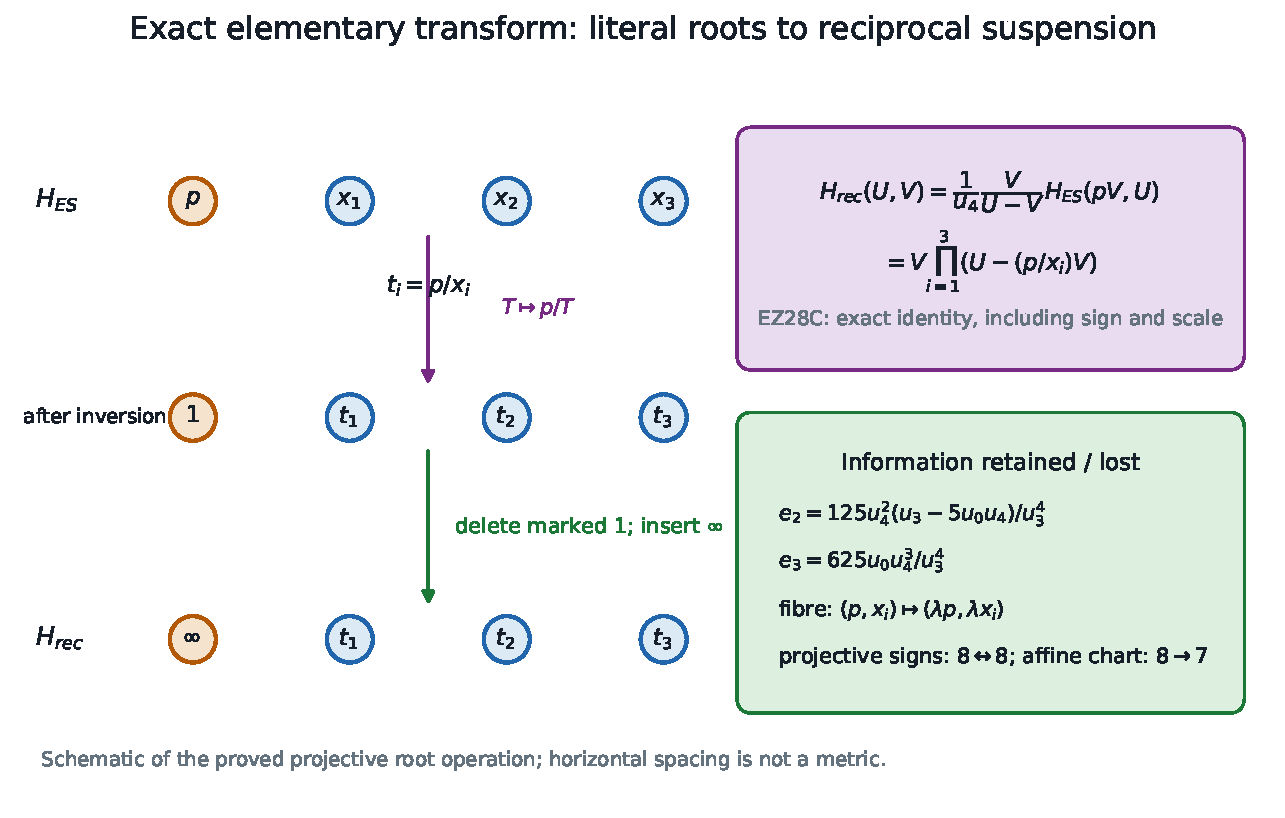
\includegraphics[width=.96\textwidth]{figures/quartic-elementary-transform.pdf}
\caption{The exact elementary transform EZ28C--EZ28O.  The drawing records
inversion \(T\mapsto p/T\), deletion of the marked root \(1\), insertion of
the root at infinity, the retained normalization, the common-scale fibre and
the signed-cover information loss.  Horizontal spacing is schematic and is
not used as a metric.  Reproduce with
\texttt{tools/generate\_20260920\_illustrations.py}.}
\label{fig:quartic-elementary-transform}
\end{figure}

\section{The prime-local seven-state fibre and its integral order}

We now specialize EZ24--28 to the original shell coordinates rather than to an
arbitrary reciprocal cubic.  In this section \(A\) denotes the original shell
denominator, so it is not the Fable source coordinate \(a\) of EZ4.  Fix a
prime \(p\equiv1\pmod4\) and retain
\begin{equation}
 \frac p4<A<\frac p2,\qquad R=4A-p,\qquad u\mid A^2,
 \qquad
 E:R\mid4u+1,\quad M:R\mid u+A.                        \tag{EZ28a}
\end{equation}
Put
\begin{equation}
 g=\gcd(A,u),\qquad
 (h,r,s)=\left(\frac{g^2}{u},\frac ug,\frac Ag\right),
 \qquad A=hrs,\quad u=hr^2,\quad\gcd(r,s)=1.           \tag{EZ28b}
\end{equation}
The ordered denominator maps, including their channel labels, are
\begin{align}
 E:\quad&\kappa=\frac{pr+s}{R},&
 (x_1,x_2,x_3)&=(A,hs\kappa,phr\kappa),\nonumber\\
 M:\quad&\lambda=\frac{r+s}{R},&
 (x_1,x_2,x_3)&=(A,phs\lambda,phr\lambda).             \tag{EZ28c}
\end{align}
They are the retained Type-I/II coordinates of Elsholtz--Tao
\cite[Section 2, Propositions 2.2 and 2.6]{ET}; multiplication gives EZ1, and
the original divisor is recovered respectively by
\begin{equation}
 u=\frac{A^2}{Rx_2-pA},\qquad
 u=\frac{pA^2}{Rx_2-pA}.                               \tag{EZ28d}
\end{equation}

\begin{lemma}[The original character survives the reciprocal map]
For every positive divisor \(d\mid A^2\), with Jacobi symbol on the left,
\begin{equation}
 \left(\frac dR\right)=\left(\frac dp\right).          \tag{EZ28e}
\end{equation}
Consequently an E state has \((h/p)=-1\), whereas an M state has
\((rs/p)=-1\).
\end{lemma}

\begin{proof}
For every odd prime \(\ell\mid A\), \(R\equiv-p\pmod\ell\), while
\(R\equiv3\pmod4\) and \(p\equiv1\pmod4\).  Quadratic reciprocity therefore
gives
\[
 \left(\frac\ell R\right)
 =\left(\frac{-1}\ell\right)\left(\frac R\ell\right)
 =\left(\frac p\ell\right)=\left(\frac\ell p\right).
\]
If \(2\mid A\), then \(R\equiv-p\pmod8\), and the supplementary law gives
\((2/R)=(2/p)\).  Multiplication with the original exponents proves EZ28e.
In E, \(u\equiv-1/4\pmod R\), hence \((u/R)=-1\); since \(u=hr^2\),
\((h/p)=-1\).  In M, \(r\equiv-s\pmod R\), so
\((r/p)=(r/R)=-(s/R)=-(s/p)\), proving the last claim.  The reciprocity and
supplementary laws used here are stated in Hatcher
\cite[Section 6.4]{Hatcher}.
\end{proof}

For the ordered reciprocal roots \(t_i=p/x_i\), write
\(f(T)=\prod_i(T-t_i)\) and \(d_i=f'(t_i)\).  The roots are simple.  In E,
\(\kappa-r=((p-R)r+s)/R>0\), \(p\kappa>s\), and \(pr>s\).  In M,
\(p\lambda>r,s\); equality \(r=s\) would force \(r=s=1\), whence
\(R\mid2\), impossible for the positive integer \(R\equiv3\pmod4\).

\begin{theorem}[Complete prime-local fibre algebra]\label{thm:local-fibre}
Choose and retain one embedding \(\ii\mapsto i_p\in\Q_p\).  The complete
affine fibre of EZ4 over the reciprocal suspension EZ25 has coordinate algebra
\begin{equation}
 \boxed{\mathcal A_{p,A,u}=
 \Q_p\times\prod_{i=1}^3
 \Q_p[\xi_i]/(\xi_i^2-d_i^{-1}).}                     \tag{EZ28f}
\end{equation}
It is reduced of dimension seven and has seven geometric points.  For an
original state its field-factor type is
\begin{equation}
 \boxed{
 E:\ \mathcal A_{p,A,u}\simeq\Q_p^3\times K_{\rm ram}^2,
 \qquad
 M:\ \mathcal A_{p,A,u}\simeq\Q_p^3\times K_{\rm unr}^2.} \tag{EZ28g}
\end{equation}
Here the two ramified factors for a fixed E state are isomorphic, but the
field is state-dependent and no canonical identification is asserted;
\(K_{\rm unr}\) is the unique unramified quadratic extension of \(\Q_p\).
In either channel there are exactly three \(\Q_p\)-rational affine points.
\end{theorem}

\begin{proof}
Write the marked factor pair as
\(L=\xi U+bV\), \(C=cU^3+dU^2V+eUV^2+f_0V^3\).  If \(\xi\ne0\), the identity
\(LC=V\prod_j(U-t_jV)\) forces, for one unique label \(i\),
\[
 L=\xi(U-t_iV),\qquad
 C=\xi^{-1}V\prod_{j\ne i}(U-t_jV).
\]
Since \(b=-\xi t_i\), the retained resultant condition is exactly
\[
 1=C(-b,\xi)=\xi^2\prod_{j\ne i}(t_i-t_j)=\xi^2d_i.
\]
Conversely either root of \(\xi^2=d_i^{-1}\) reconstructs the unique source
point by EZ13.  At \(\xi=0\), the four target equations successively force the
single point EZ26.  The source Jacobian is the constant \(-2\), a \(p\)-adic
unit, so all factors are reduced.  This proves EZ28f.

For E put \(H=hrs\kappa\).  In the original order
\begin{equation}
 (t_1,t_2,t_3)=H^{-1}(p\kappa,pr,s),                    \tag{EZ28h}
\end{equation}
and direct subtraction gives
\begin{equation}
 (d_1,d_2,d_3)=H^{-2}\bigl(
 p(\kappa-r)(p\kappa-s),
 -p(\kappa-r)(pr-s),
 (p\kappa-s)(pr-s)\bigr).                             \tag{EZ28i}
\end{equation}
The identity \(pD+1=4hr\kappa\) makes \(\kappa\) a unit.  If
\(p\mid\kappa-r\), it would give \(4hr^2\equiv1\pmod p\), contradicting
\((h/p)=-1\).  Hence
\begin{equation}
 (v_p(d_1),v_p(d_2),v_p(d_3))=(1,1,0),\qquad
 \frac{d_1}{d_2}\equiv-1,\quad d_3\equiv16\pmod p.    \tag{EZ28j}
\end{equation}
Because \(-1\) is a square in \(\Q_p\), the first two quadratic factors are
isomorphic ramified fields and the third splits.

For M put \(H=hrs\lambda\).  Then
\begin{equation}
 (t_1,t_2,t_3)=H^{-1}(p\lambda,r,s),\qquad
 (d_1,d_2,d_3)\sim(rs,r(r-s),s(s-r))\pmod p,           \tag{EZ28k}
\end{equation}
where the omitted common factor \(H^{-2}\) is a square unit.  By EZ28e,
\(d_1\) is a nonsquare unit, while
\(d_1d_2d_3\sim-r^2s^2(r-s)^2\) is a square.  Exactly one of labels \(2,3\)
is square and the other is nonsquare; the complement \(r\leftrightarrow s\)
exchanges those labels.  Thus one finite quadratic splits and two give the
same unramified quadratic field.  Adding the infinity factor proves EZ28g and
the count of three rational points.  The square-unit lift and the
ramified/unramified classification used here are the elementary Hensel and
local-extension results in Milne \cite[Chapter 7]{Milne}; explicitly, a unit
square root lifts by
\[
 b_{n+1}=b_n+p^nt,\qquad
 t\equiv-(b_n^2-z)p^{-n}(2b_n)^{-1}\pmod p.
\]
\end{proof}

\begin{theorem}[Exact integral root order and one-prime loss]
Let \(\mathcal O_E\) and \(\mathcal O_M\) be the images of
\(\Z_p[T]/(f)\) under evaluation at the ordered roots.  Then
\begin{equation}
 \boxed{\mathcal O_E=
 \{(z_1,z_2,z_3)\in\Z_p^3:z_1\equiv z_2\pmod p\},
 \qquad \mathcal O_M=\Z_p^3.}                          \tag{EZ28l}
\end{equation}
The normalization quotient and conductor are
\begin{equation}
 0\longrightarrow\mathcal O_E\longrightarrow\Z_p^3
 \xrightarrow{z_1-z_2\bmod p}\F_p\longrightarrow0,
 \qquad
 \mathfrak f_E=p\Z_p\times p\Z_p\times\Z_p.          \tag{EZ28m}
\end{equation}
The sequence has no \(\Z_p\)-linear right inverse.  For any same-prime E and M
states, the unique labelled quadratic interpolations \(F(t_i^E)=t_i^M\) and
\(G(t_i^M)=t_i^E\) satisfy
\begin{equation}
 (v_p(F_0),v_p(F_1),v_p(F_2))=(0,-1,-1),\qquad
 G\in\Z_p[T],\qquad pF(T)\equiv cT(T-4)\pmod p         \tag{EZ28n}
\end{equation}
for a nonzero \(c\in\F_p\).  Their composition congruences are divisibilities
in \(\Q_p[T]\), not generally in \(\Z_p[T]\).
\end{theorem}

\begin{proof}
In E, EZ28h--j give
\(v_p(t_1-t_2)=1\), the other two difference valuations zero, and
\((t_1,t_2,t_3)\equiv(0,0,4)\pmod p\).  Evaluation therefore forces the
congruence in EZ28l.  Conversely, for a tuple satisfying it, the polynomial
\[
 L(T)=z_1+\frac{z_2-z_1}{t_2-t_1}(T-t_1)
\]
is integral, and
\[
 L(T)+\frac{z_3-L(t_3)}{(t_3-t_1)(t_3-t_2)}
             (T-t_1)(T-t_2)
\]
is an integral interpolant.  In M all three differences are units, so the
Vandermonde interpolation is integral and surjective.  The quotient map in
EZ28m is therefore exact.  An element of \(\Z_p^3\) multiplies all of
\(\Z_p^3\) into \(\mathcal O_E\) exactly when its first two coordinates are
divisible by \(p\), proving the conductor formula.  A right inverse
\(\F_p\to\Z_p^3\) would have \(p\)-torsion image, but \(\Z_p^3\) is
torsion-free.

For interpolation write
\[
 F(T)=\sum_i t_i^M
 \frac{(T-t_j^E)(T-t_k^E)}{(t_i^E-t_j^E)(t_i^E-t_k^E)}.
\]
The E denominators have valuations \((1,1,0)\), whereas the M roots have
valuations \((1,0,0)\).  Multiplication by \(p\) leaves only the \(i=2\) term
modulo \(p\), giving the last congruence in EZ28n and the linear and quadratic
valuations \(-1\).  The three contributions to the constant term have
valuations \(1,0,2\); the unique minimum cannot cancel, so \(v_p(F_0)=0\).
All M difference denominators are units, proving \(G\in\Z_p[T]\).  Each
composition fixes three distinct roots, hence
\(f_E\mid G(F(T))-T\) and \(f_M\mid F(G(T))-T\) in \(\Q_p[T]\).  The exact
denominator just proved prevents upgrading this assertion in general to
\(\Z_p[T]\).
\end{proof}

\begin{corollary}[The same rational point count hides different specialization]
For E,
\begin{equation}
 v_p(\sigma_2,\sigma_3,\Disc f)=(1,2,2),\qquad
 \bar f=T^2(T-4).                                      \tag{EZ28o}
\end{equation}
The four signed branches over \(t_1,t_2\) have
\begin{equation}
 (v_p(\xi),v_p(y_0),v_p(z_0),v_p(w_0))
 =(-1/2,1/2,1,1),                                      \tag{EZ28p}
\end{equation}
so they escape the affine integral chart.  The reduced special fibre consists
exactly of
\begin{equation}
\begin{aligned}
 &(0,-4,56i_p,-704),\\
 &(1/4,-4-4i_p,32+48i_p,-1152-384i_p),\\
 &(-1/4,-4+4i_p,-32+48i_p,-1152+384i_p).
\end{aligned}                                             \tag{EZ28q}
\end{equation}
For M, \(v_p(\sigma_2,\sigma_3,\Disc f)=(0,1,0)\); all seven geometric
branches are integral and remain distinct.  In both channels exactly three
special-fibre points are \(\F_p\)-rational.  The M roots have distinct
reductions and all derivatives are units; their derivative residues need not
be pairwise distinct.
\end{corollary}

\begin{proof}
For E, \(\kappa+r=sD\), \(D\) is a unit, and the elementary symmetric
expressions from EZ28h give the valuations in EZ28o.  EZ28j and the inverse
EZ13 have unique lowest-valuation terms
\(-i_p/\xi\), \(3i_p/\xi^2\), and \(-4/\xi^2\), proving EZ28p.
Reduction has \(t_3=4\), \(d_3=16\), so \(\xi=\pm1/4\); substitution in
EZ13 and EZ26 gives EZ28q.  The double root zero has no finite inverse because
\(\xi^2\bar f'(0)=1\) is impossible.  For M, EZ28k has three distinct root
reductions and unit derivatives, proving the remaining assertions.  For
example, the valid state
\(p=5,(A,u,R,h,r,s,\lambda,H)=(2,1,3,1,1,2,1,2)\) has root residues
\((0,3,1)\) but derivative residues \((3,1,3)\), so no stronger distinctness
claim is made.
\end{proof}

The conductor in EZ28m is the conductor of an integral root order in its
normalization.  It is not the fixed complex weighted operator of EZ29--35.
The rational interpolation proves an exact morphism between already occupied
channel targets; it does not create a missing source state.

\section{A same-prime negative-square target change}

Return to an original E state and put
\begin{equation}
 D=\frac{4u+1}{R},\qquad v=hs^2,\qquad
 \alpha=v-R,\qquad\beta=v-D.                           \tag{EZ28r}
\end{equation}
The retained identities are
\begin{equation}
 h\mid\alpha\beta-1,\qquad p\equiv\alpha\pmod h,
 \qquad p\beta\equiv1\pmod h.                         \tag{EZ28s}
\end{equation}

\begin{theorem}[Negative-four-square channel transfer]
Suppose \(\alpha=-4c^2\) or \(\beta=-4c^2\) for an integer \(c>0\).  Then
\(h\equiv3\pmod4\) and \(\gcd(h,c)=1\).  Put \(j=(h+1)/4\).  On the exact
selected-word domain \(c\mid j\), define
\begin{equation}
 Q=h,\qquad
 U=\begin{cases}c^2,&\alpha=-4c^2,\\(j/c)^2,&\beta=-4c^2,\end{cases}
 \qquad R_M=\frac{p+4U}{h},\qquad A_M=\frac{p+R_M}{4}.  \tag{EZ28t}
\end{equation}
Then \((p,A_M,R_M,U)\) is an original M state.  With
\(g_M=\gcd(j,U)\), its complete normalization and ordered denominators are
\begin{equation}
 h_M=\frac{g_M^2}{U},\quad r_M=\frac{U}{g_M},\quad
 \lambda_M=\frac{j}{g_M},\quad s_M=R_M\lambda_M-r_M,   \tag{EZ28u}
\end{equation}
\begin{equation}
 \boxed{(A_M,\;p h_Ms_M\lambda_M,\;p h_Mr_M\lambda_M).} \tag{EZ28v}
\end{equation}
Writing \(j=cm\) and \(d=\gcd(c,m)\), the alpha branch has
\((h_M,r_M,\lambda_M)=(d^2,c/d,m/d)\), while the beta branch has
\((d^2,m/d,c/d)\).  Thus \(h_M=d^2\) is a square.  In particular, every
already-existing E state on \(\alpha=-4\) or \(\beta=-4\) returns to M, with
no bound on the other shape coordinate.  This last statement neither produces
source states on those lines nor asserts that there are infinitely many.
\end{theorem}

\begin{proof}
If \(\alpha=-4c^2\), then \(R=hs^2+4c^2\equiv3\pmod4\).  If
\(\beta=-4c^2\), then \(D=hs^2+4c^2\), and
\(RD=4hr^2+1\equiv1\pmod4\) with \(R\equiv3\pmod4\), so
\(D\equiv3\pmod4\).  In either case \(s\) is odd and \(h\equiv3\pmod4\).
Equation EZ28s makes \(h\) coprime to \(c\).

In the alpha branch \(h\mid p+4c^2\).  In the beta branch,
\(-4pc^2\equiv1\pmod h\); since \(4j\equiv1\pmod h\) and \(c\mid j\),
\(h\mid p+4(j/c)^2\).  Hence \(R_M\) is integral.  The original alpha
inequality gives \(4U<p-h<(h-1)p\); in beta,
\(4U\le(h+1)^2/4<2h(h-1)<p(h-1)\).  Thus \(0<R_M<p\).  Moreover
\(hR_M\equiv1\pmod4\), so \(R_M\equiv3\pmod4\) and
\(p/4<A_M<p/2\).

Since \(p=hR_M-4U\),
\[
 A_M=jR_M-U,\qquad A_M+U=jR_M,
\]
and \(U\mid j^2\) gives \(U\mid A_M^2\).  This is exactly the original M
gate.  Any common divisor of \(R_M,U\) divides \(p\), while
\(0<R_M<p\), so \(\gcd(R_M,U)=1\).  It follows that
\(\gcd(A_M,U)=\gcd(j,U)=g_M\), and direct substitution proves EZ28u,
\(A_M=h_Mr_Ms_M\), \(U=h_Mr_M^2\), and
\(r_M+s_M=R_M\lambda_M\).  These identities prove the original primitive
normalization and EZ28v.  The formulas with \(j=cm\) follow by taking
\(d=\gcd(c,m)\).
\end{proof}

The inverse fibres are also exact.  In the alpha branch put
\(N=(p+4c^2)/h\).  For every positive divisor \(s\mid N\), set
\begin{equation}
 k=N/s,\qquad r=(s+k)/4,\qquad R_s=hs^2+4c^2.          \tag{EZ28w}
\end{equation}
The complete source fibre consists precisely of those divisors for which
\begin{equation}
 s+k\equiv0\pmod4,\qquad\gcd(r,s)=1,\qquad R_s<p,
 \qquad\boxed{R_s\mid4hr^2+1}.                         \tag{EZ28x}
\end{equation}
The boxed condition is the original E gate and cannot be omitted.  With
\(D_s=(4hr^2+1)/R_s\), it gives
\(\kappa=sD_s-r=(pr+s)/R_s\); conversely these formulas reconstruct the
entire original E state and \(\alpha=-4c^2\).  At \(p=5209,h=95,c=2\), the
candidate \(s=5,k=11,r=4\) passes the other tests but has
\(R_s=2391\nmid6081=4hr^2+1\), proving that the gate is material.

In the beta branch put
\begin{equation}
 F_0=\frac{4c^2p+1}{h},\qquad D_s=hs^2+4c^2,\qquad
 \Delta_s=s^2(D_s^2-p)-F_0.                            \tag{EZ28y}
\end{equation}
For \(1\le s\le\lfloor(p-1)/(2h)\rfloor\), retain exactly the positive
squares \(k^2=\Delta_s\) for which \(sD_s-k\) is positive and even, put
\(r=(sD_s-k)/2\), \(\kappa=(sD_s+k)/2\), and retain the original coprimality
and first-half inequalities.  The identity
\(4hr\kappa=pD_s+1\) then proves both directions, including the original E
divisibility; there is no omitted gate in this branch.

Finally, equality of full selected targets first recovers the common
\(Q=4h_Mr_M\lambda_M-1=h\).  For this fixed \(h\), an alpha label \(c_1\)
and beta label \(c_2\) select the same \(U\) exactly when
\begin{equation}
 c_1c_2=j.                                              \tag{EZ28z}
\end{equation}
Different sources in one fibre remain distinct until a stated pushforward;
the kernel of that pushforward is generated by their same-target differences.
The complete independent review and corrected build are preserved in
\cite{Turn7Fabel}.

\section{The complete fixed-cofactor middle fibre}

The two selected square words above belong to a larger finite fibre.  Keeping
the original E-state variables fixed, suppose \(h\equiv3\pmod4\), and put

\begin{equation}
 j=\frac{h+1}{4},\qquad
 \mathcal U_{p,h}=\{U\in\mathbb Z_{>0}:U\mid j^2,\ h\mid p+4U\}.
                                                               \tag{EZ28P}
\end{equation}

\begin{theorem}[Complete fixed-\(Q\) middle fibre]
For each \(U\in\mathcal U_{p,h}\), define
\begin{align}
 R_U&=\frac{p+4U}{h},& A_U&=\frac{p+R_U}{4},&g_U&=\gcd(j,U),\notag\\
 h_U&=\frac{g_U^2}{U},&r_U&=\frac{U}{g_U},&
 \lambda_U&=\frac{j}{g_U},&s_U&=R_U\lambda_U-r_U.       \tag{EZ28Q}
\end{align}
Then \((A_U,R_U,U,h_U,r_U,s_U,\lambda_U)\) is an original M state
at \(p\), and its normalized cofactor is

\begin{equation}
 Q_U=4h_Ur_U\lambda_U-1=h,                              \tag{EZ28R}
\end{equation}

and its ordered ES denominators are

\begin{equation}
 \boxed{\left(A_U,\;p h_Us_U\lambda_U,\;
                    p h_Ur_U\lambda_U\right).}          \tag{EZ28S}
\end{equation}

The assignment is a bijection from \(\mathcal U_{p,h}\) onto all original M
states at \(p\) whose normalized cofactor is \(Q=h\).
\end{theorem}

\begin{proof}
An original E state has \(h\le A<p/2\), so \(p>2h\); here \(h\ge3\).
Since \(U\mid j^2\),

\[
 4U\le4j^2=\frac{(h+1)^2}{4}<2h(h-1)<p(h-1).
\]

Hence \(0<R_U<p\).  Moreover \(hR_U=p+4U\equiv1\pmod4\); because
\(p\equiv1\pmod4\) and \(h\equiv3\pmod4\),
\(R_U\equiv3\pmod4\).  Thus \(A_U\) is integral and
\(p/4<A_U<p/2\).

Prime by prime, \(U\mid j^2\) implies \(g_U^2/U\in\mathbb Z_{>0}\).
The definitions give

\[
 h_Ur_U=g_U,\qquad h_Ur_U^2=U,\qquad
 h_Ur_U\lambda_U=j,
\]

and

\[
 R_Uj-U=\frac{R_U(h+1)}4-U=\frac{p+R_U}{4}=A_U.
\]

Consequently \(h_Ur_Us_U=A_U\), \(r_U+s_U=R_U\lambda_U\),
\(A_U+U=R_Uj\), and \(U\mid A_U^2\).  Also
\(\gcd(r_U,\lambda_U)=1\).  If a prime divided both \(r_U\) and \(s_U\),
it would divide \(R_U\), then \(hR_U-4U=p\); this is impossible because
\(0<R_U<p\).  Hence \(\gcd(r_U,s_U)=1\).  These are precisely the original
M gates, and EZ28R and EZ28S follow by substitution.

Conversely, let an original M state have cofactor \(Q=h\), written

\[
 A_M=h_Mr_Ms_M,\qquad U=h_Mr_M^2,\qquad
 \lambda_M=\frac{r_M+s_M}{R_M}.
\]

Then

\[
 j=\frac{h+1}{4}=h_Mr_M\lambda_M,qquad
 \frac{j^2}{U}=h_M\lambda_M^2\in\mathbb Z_{>0},
\]

so \(U\mid j^2\).  Furthermore

\[
 A_M+U=h_Mr_M(r_M+s_M)=R_Mj,qquad
 p+4U=4(A_M+U)-R_M=R_Mh.
\]

Thus \(U\in\mathcal U_{p,h}\).  The primitive normalization gives
\(\gcd(j,U)=h_Mr_M\), and EZ28Q recovers
\((h_M,r_M,\lambda_M,s_M)\) exactly.  The original middle divisor \(U\)
separates distinct states, proving bijectivity.
\end{proof}

\begin{corollary}[Exact negative-square slices and emptiness]
If the existing E state has \(\alpha=-4c^2\) or \(\beta=-4c^2\), then

\begin{align}
 \alpha=-4c^2:\quad
 \mathcal U_{p,h}&=\{U\mid j^2:U\equiv c^2\pmod h\},\notag\\
 \beta=-4c^2:\quad
 \mathcal U_{p,h}&=\{U\mid j^2:c^2U\equiv j^2\pmod h\}. \tag{EZ28T}
\end{align}

The selected words \(U=c^2\) and \(U=(j/c)^2\) exist exactly when
\(c\mid j\), but that divisibility is not necessary for the complete fibre to
be nonempty.  With

\[
 \Delta_h=\{U\bmod h:U\mid j^2\},
\]

the exact criterion is

\begin{equation}
 \boxed{\mathcal U_{p,h}=\varnothing\iff
 -p\,4^{-1}\pmod h\notin\Delta_h.}                    \tag{EZ28U}
\end{equation}
\end{corollary}

\begin{proof}
In the alpha branch, \(p\equiv-4c^2\pmod h\), so the defining congruence
\(p+4U\equiv0\pmod h\) is equivalent to \(U\equiv c^2\pmod h\).
In the beta branch, \(-4c^2p\equiv1\pmod h\).  Multiplying the defining
congruence by \(4c^2\) and using \(4j\equiv1\pmod h\) yields
\(c^2U\equiv j^2\pmod h\); every step is reversible because
\(\gcd(4c^2,h)=1\).  Formula EZ28U is the defining congruence solved for
\(U\bmod h\).
\end{proof}

Let \(\mathcal E_p\) be the original E-state set at a hard prime.  After the
proved diagonal return and every fixed-\(Q\) return, the exact residual source
is

\begin{equation}
 \boxed{\mathcal E_p^{\rm res}=
 \{e\in\mathcal E_p:R\ne D,
 \quad [h\not\equiv3\pmod4\text{ or }\mathcal U_{p,h}=\varnothing]\}.} \tag{EZ28V}
\end{equation}

The shape-rigidity theorem of \cite{Turn7} states that radius at most seven
is the diagonal profile \((\alpha,\beta)=(-1,-1)\), while the only
nonsingular radius-eight profile is \((8,-4,11)\).  For the latter,
\(j=3\) and \(U=9\in\mathcal U_{p,11}\), so EZ28Q gives

\begin{equation}
 (h_U,r_U,s_U,\lambda_U)=\left(1,3,\frac{p+3}{11},1\right),
 \quad A_U=\frac{3(p+3)}{11},\quad R_U=\frac{p+36}{11}. \tag{EZ28W}
\end{equation}

Therefore every state remaining in EZ28V has
\(\max(|\alpha|,|\beta|)\ge9\).  If such a residual state still has a
negative-square coordinate, EZ28T fails for every divisor \(U\mid j^2\), a
strict finite exclusion stronger than failure of the selected word.

This improvement is strict.  At the certified prime \(p=41161\), the E state

\[
 (A,R,u,h,r,s,\kappa,D,\alpha,\beta)
 =(10318,111,9678284,11,938,1,347829,348767,-100,-348756)
\]

has \(j=3\), \(c=5\nmid j\), but \(U=3\in\mathcal U_{41161,11}\).
The resulting M state and exact decomposition are

\begin{equation}
\begin{aligned}
 (A_U,R_U,U,h_U,r_U,s_U,\lambda_U)
   &=(11226,3743,3,3,1,3742,1),\\
 \boxed{\frac4{41161}}
   &=\boxed{\frac1{11226}+\frac1{462073386}+\frac1{123483}}.
\end{aligned}                                             \tag{EZ28X}
\end{equation}

Primality follows from the Lucas witness \(22\): \(22^{41160}\equiv1\)
modulo \(41161\), while for \(q=2,3,5,7\) the residues
\(22^{41160/q}\) are \(41160,40429,26424,13707\), each with predecessor
coprime to \(41161\).  Conversely, \(p=3049,h=31,j=8,c=6\) has
\(\{U\bmod31:U\mid64\}=\{1,2,4,8,16\}\) but \(c^2\equiv5\pmod{31}\);
its alpha slice is empty.  Thus a negative-square coordinate alone does not
force a fixed-(Q) return.  The executable exact comparison with every
recorded original M state is retained in \cite{Turn7Fabel}.

\input{CAPACITY_COMPLETION}

\begin{figure}[htbp]
\centering
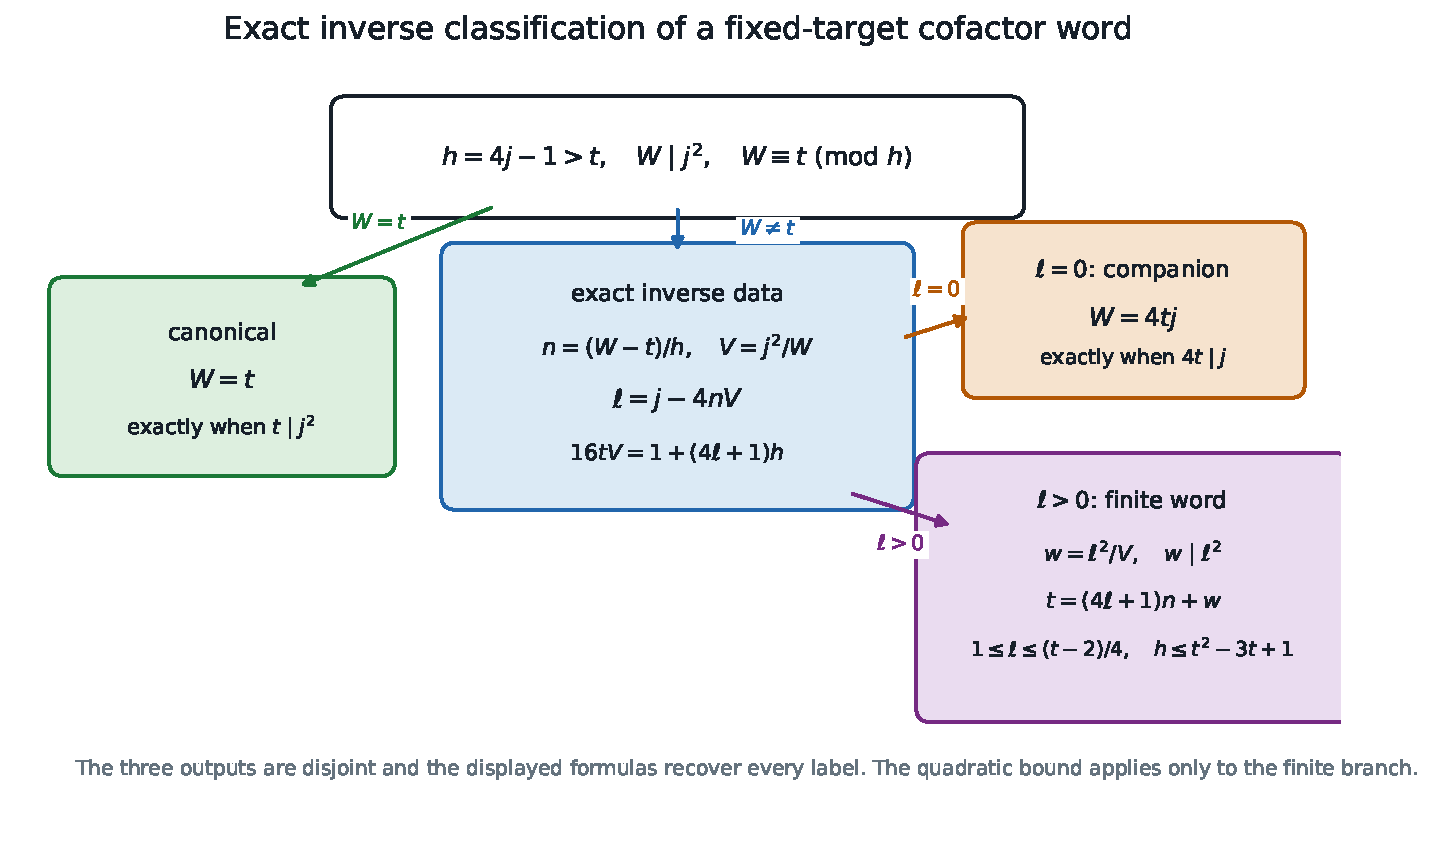
\includegraphics[width=\textwidth]{figures/fixed-target-capacity-partition.pdf}
\caption{The exact inverse in Theorem~\ref{thm:capacity}. Starting from a
word \(W\), equations (9)--(10) recover \(n,V,\ell\), while the signs and
domains separate the canonical, companion and finite branches. The sharp
grade bound belongs only to the finite branch.}
\label{fig:capacity-partition}
\end{figure}

\begin{figure}[htbp]
\centering
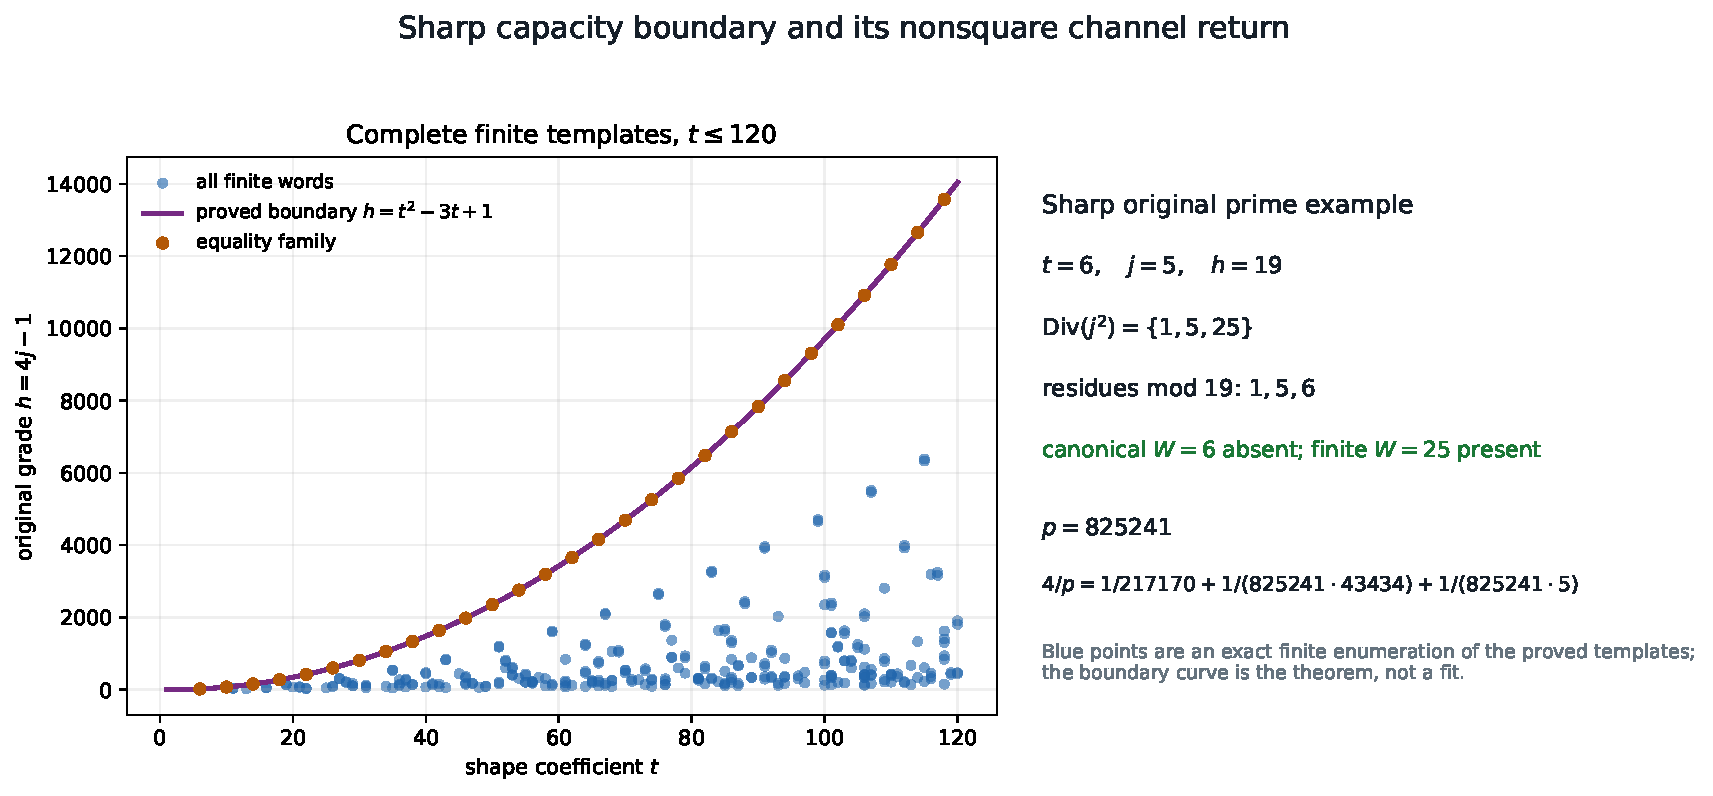
\includegraphics[width=\textwidth]{figures/capacity-sharp-bound.pdf}
\caption{Every finite template with \(t\le120\), plotted against the proved
boundary in Theorem~\ref{thm:bound}. The right panel retains the exact
\(p=825241\) nonsquare return from equations (17)--(18). The points are a
reproducible enumeration by
\texttt{tools/generate\_20260920\_illustrations.py}; the curve is the proved
bound, not an empirical fit.}
\label{fig:capacity-bound}
\end{figure}

\section{The exact bridge to a fixed weighted conductor}

Fix one reference arithmetic quartet with distinct roots
\(\rho_{*,1},\ldots,\rho_{*,4}\), its original exponential polynomial,
first nonzero moment \(\mu_v\), period frame and Taylor unit.  Let
\begin{equation}
 V_*=(\rho_{*,j}^{\,n})_{0\le n\le3,\,1\le j\le4},\qquad
 (B_{v,*})_{kj}=\begin{cases}
 \binom{v+j}{k}\mu_{v+j-k},&0\le k\le j\le3,\\
 0,&k>j,
 \end{cases}                                           \tag{EZ29}
\end{equation}
and retain the source frame
\begin{equation}
 K=\begin{pmatrix}
 0&\ii&1/\sqrt2&1/\sqrt2\\
 0&-1&-1-\sqrt2\ii&1-\sqrt2\ii\\
 \ii/2&-3\ii&2\sqrt2+6\ii&-2\sqrt2+6\ii\\
 0&13&-34-19\sqrt2\ii&34-19\sqrt2\ii
 \end{pmatrix}.                                        \tag{EZ30}
\end{equation}
Define
\begin{equation}
 \Phi_*=(V_*^{\mathsf T})^{-1}K^{-1},\qquad
 \Psi_*=B_{v,*}(V_*^{\mathsf T})^{-1}K^{-1}.           \tag{EZ31}
\end{equation}
The columns of \(K\) are the auxiliary labelled source frame; they are not
identified with either \(p,x,y,z\) or the reference roots.  The original
weighted conductor is \(T_{A,*}|_{\mathcal U_*}\), and the exact square is
\begin{equation}
 T_{A,*}\Phi_*=\Psi_*.                                  \tag{EZ32}
\end{equation}
The receiving map \(\Psi_*\) is not itself the conductor.

\begin{theorem}[Conductor transport of the ES quartic]
All three maps in EZ32 are invertible and have zero kernel.  Put
\begin{equation}
 P_{\mathcal U,*}=\Phi_*P\Phi_*^{-1},\qquad
 P_{\mathcal W,*}=\Psi_*P\Psi_*^{-1}.                  \tag{EZ33}
\end{equation}
For every target \(u\) and source point \(q\) with \(P(q)=u\),
\begin{equation}
 P_{\mathcal U,*}(\Phi_*q)=\Phi_*u,qquad
 P_{\mathcal W,*}(\Psi_*q)=\Psi_*u,qquad
 T_{A,*}P_{\mathcal U,*}=P_{\mathcal W,*}T_{A,*}.      \tag{EZ34}
\end{equation}
In particular the eight points EZ13 above \(J_4\), their deck involution,
and the exceptional set EZ28 pass bijectively to the fixed conductor planes.
\end{theorem}

\begin{proof}
Distinct reference roots make \(V_*\) invertible.  Moreover
\[
 \det B_{v,*}=\mu_v^4\prod_{j=0}^3\binom{v+j}{v}\ne0,
 \qquad \det K=77\sqrt2\,\ii/2.
\]
Thus EZ31 is invertible and EZ32 is the exact conductor identity proved in
\cite[FC26--FC35]{SignedCover}.  The first two identities in EZ34 are the
definitions of conjugacy.  Inserting EZ32 between them proves the last one.
Invertible linear maps preserve fibres, escaping sequences, convergence and
deck equations, proving the final assertion.
\end{proof}

The coefficient hypersurface itself also transports, with no loss of its
arithmetic coordinates.  Define the two inverse matrices
\begin{equation}
 R_{\mathcal U}:=\Phi_*^{-1}=KV_*^{\mathsf T},\qquad
 R_{\mathcal W}:=\Psi_*^{-1}=KV_*^{\mathsf T}B_{v,*}^{-1}.       \tag{EZ34a}
\end{equation}
For \(\mathcal C\in\{\mathcal U,\mathcal W\}\), let
\(\ell^{\mathcal C}_0,\ell^{\mathcal C}_2,
\ell^{\mathcal C}_3,\ell^{\mathcal C}_4\) be the four row covectors of
\(R_{\mathcal C}\), in the retained coefficient order
\((u_0,u_2,u_3,u_4)\).

\begin{theorem}[Exact equation in the fixed zeta receiving coordinates]
In either fixed conductor plane, the transported arithmetic image is the
irreducible quartic hypersurface
\begin{align}
 G_{\mathcal C}(q):={}&
 625\ell^{\mathcal C}_0(q)\ell^{\mathcal C}_4(q)^3
 -125\ell^{\mathcal C}_3(q)\ell^{\mathcal C}_4(q)^2\nonumber\\
 &+25\ell^{\mathcal C}_2(q)\ell^{\mathcal C}_3(q)^2
                    \ell^{\mathcal C}_4(q)
 -4\ell^{\mathcal C}_3(q)^4=0.                       \tag{EZ34b}
\end{align}
On the open chart where
\(\ell^{\mathcal C}_0\ell^{\mathcal C}_3
\ell^{\mathcal C}_4\ne0\), its exact inverse arithmetic coordinates are
\begin{align}
 p&=-5\frac{\ell^{\mathcal C}_4}{\ell^{\mathcal C}_3},&
 s_1&=-\frac1{\ell^{\mathcal C}_0}
          +5\frac{\ell^{\mathcal C}_4}{\ell^{\mathcal C}_3},\nonumber\\
 s_2&=\frac{4(\ell^{\mathcal C}_3)^2}
              {25\ell^{\mathcal C}_0\ell^{\mathcal C}_4},&
 s_3&=-\frac{\ell^{\mathcal C}_3}
             {5\ell^{\mathcal C}_0}.                 \tag{EZ34c}
\end{align}
The reduced singular support of EZ34b is the codimension-two linear plane
\begin{equation}
 \ell^{\mathcal C}_3=\ell^{\mathcal C}_4=0.           \tag{EZ34d}
\end{equation}
Finally, the original conductor carries these equations and recovered
coordinates identically:
\begin{equation}
 G_{\mathcal W}(T_{A,*}q)=G_{\mathcal U}(q),\qquad
 \ell_j^{\mathcal W}(T_{A,*}q)=\ell_j^{\mathcal U}(q)
 \quad(j=0,2,3,4).                                    \tag{EZ34e}
\end{equation}
\end{theorem}

\begin{proof}
For a coefficient column \(u\), EZ34a gives
\(R_{\mathcal U}\Phi_*u=u\) and
\(R_{\mathcal W}\Psi_*u=u\).  Thus each retained covector recovers the
corresponding literal coefficient, and substituting these four identities
into EZ9 and EZ9c proves EZ34b--EZ34c.  An invertible linear change of
coordinates preserves irreducibility and carries the reduced singular plane
\(u_3=u_4=0\) exactly to EZ34d.  From
\(T_{A,*}=\Psi_*\Phi_*^{-1}\) one has
\(R_{\mathcal W}T_{A,*}=R_{\mathcal U}\); applying each row and then the
quartic polynomial proves EZ34e.
\end{proof}

We now write every receiver covector in EZ34b without hiding the inverse
matrix.  Use the fixed Time order
\((\mathrm M,\mathrm N,\mathrm T,\mathrm E)\), write
\(m_j=\mu_{v+j}\), and put
\[
 \alpha_2=\binom{v+2}{2},\qquad
 \alpha_3=\binom{v+3}{3},\qquad
 \beta_{23}=\binom{v+3}{2}.
\]
For a receiver coefficient column
\(\mathbf r=(r_0,r_1,r_2,r_3)^{\mathsf T}\), define successively
\begin{align}
 c_3&=\frac{r_3}{\alpha_3m_0},\nonumber\\
 c_2&=\frac{r_2-\beta_{23}m_1c_3}{\alpha_2m_0},\nonumber\\
 c_1&=\frac{r_1-(v+2)m_1c_2-(v+3)m_2c_3}{(v+1)m_0},\nonumber\\
 c_0&=\frac{r_0-m_1c_1-m_2c_2-m_3c_3}{m_0},          \tag{EZ34f}\\
 \xi_a(\mathbf r)&=c_0+c_1\rho_{*,a}+c_2\rho_{*,a}^2
                         +c_3\rho_{*,a}^3
 \quad(a=\mathrm M,\mathrm N,\mathrm T,\mathrm E).   \tag{EZ34g}
\end{align}
The four literal coefficient-recovery forms are
\begin{align}
 U_0={}&\ii\xi_{\mathrm N}
       +\frac{\xi_{\mathrm T}+\xi_{\mathrm E}}{\sqrt2},\nonumber\\
 U_2={}&-\xi_{\mathrm N}+(-1-\sqrt2\ii)\xi_{\mathrm T}
       +(1-\sqrt2\ii)\xi_{\mathrm E},\nonumber\\
 U_3={}&\frac{\ii}{2}\xi_{\mathrm M}-3\ii\xi_{\mathrm N}
       +(2\sqrt2+6\ii)\xi_{\mathrm T}
       +(-2\sqrt2+6\ii)\xi_{\mathrm E},\nonumber\\
 U_4={}&13\xi_{\mathrm N}+(-34-19\sqrt2\ii)\xi_{\mathrm T}
       +(34-19\sqrt2\ii)\xi_{\mathrm E}.            \tag{EZ34h}
\end{align}
Indeed EZ34f is forward substitution in
\(B_{v,*}c=\mathbf r\), EZ34g is
\(V_*^{\mathsf T}c\), and EZ34h is multiplication by the four rows of
\(K\).  Hence \(U_j(\mathbf r)=\ell_j^{\mathcal W}(\mathbf r)\) exactly.
In particular
\begin{equation}
 F_*(\mathbf r):=625U_0U_4^3-125U_3U_4^2
             +25U_2U_3^2U_4-4U_3^4                 \tag{EZ34i}
\end{equation}
is the fully expanded-by-rows form of \(G_{\mathcal W}\); no coefficient
has been fitted to an ES example.  It is nonzero and irreducible, has total
degree four and retains the nonzero cubic term \(-125U_3U_4^2\).

\begin{theorem}[Prime-marked receiver pair and polynomial selector]
Assume
\begin{equation}
 F_*(\mathbf r)=0,qquad
 U_0U_3U_4\Disc(H_{\mathbf r})\ne0,qquad
 p=-\frac{5U_4}{U_3},                                \tag{EZ34j}
\end{equation}
where
\[
 H_{\mathbf r}(U,V)=U_0U^4+U^3V+U_2U^2V^2+U_3UV^3+U_4V^4.
\]
Then
\begin{align*}
 H_{\mathbf r}(U,V)&=(U-pV)Q_{\mathbf r,p}(U,V),\\
 Q_{\mathbf r,p}(U,V)&=U_0U^3+(1+pU_0)U^2V\\
 &\quad +(U_2+p+p^2U_0)UV^2
 +(U_3+pU_2+p^2+p^3U_0)V^3.
\end{align*}
Put
\[
 \kappa=4U_0p^3+3p^2+2U_2p+U_3=h_{\mathbf r}'(p).
\]
It is nonzero by the discriminant hypothesis.  For each of the two choices
\(A^2\kappa=1\), define
\[
 L_A=A(U-pV),\qquad C_A=A^{-1}Q_{\mathbf r,p}.
\]
Their six factor coordinates are
\begin{equation}
 (a,b,c,d,e,f)=
 \left(A,-Ap,\frac{U_0}{A},\frac{1+pU_0}{A},
 \frac{U_2+p+p^2U_0}{A},
 \frac{U_3+pU_2+p^2+p^3U_0}{A}\right).               \tag{EZ34k}
\end{equation}
They satisfy, without a changed resultant convention,
\begin{equation}
 L_AC_A=H_{\mathbf r},\quad
 \Res(L_A,C_A)=1,\quad ad+bc=1,
 \quad4af-be=-\frac{F_*(\mathbf r)}{U_3^3}=0.         \tag{EZ34l}
\end{equation}
The corresponding original source points are
\begin{align}
 q_A(\mathbf r)=\Bigg(&A,-p-\frac{\ii}{A},
 \frac{U_0}{A^3}+\frac{2p}{A}+\frac{3\ii}{A^2},\nonumber\\
 &\frac{7\ii p^2}{A}
 +\frac{U_2-17p+U_0p^2}{A^2}
 -\frac{13\ii}{A^3}-\frac{2U_0}{A^4}\Bigg),          \tag{EZ34m}
\end{align}
and the two receiver-source points are \(z_A=\Psi_*q_A\).

More intrinsically, let \(z\) be any of the eight points over \(\mathbf r\)
under \(P_{\mathcal W,*}\), and decode
\((A(z),Y(z),Z(z),\Omega(z))^{\mathsf T}=\Psi_*^{-1}z\).
Then (z) is one of the two points marking (p) if and only if
\begin{equation}
 5A(z)U_4(\mathbf r)-A(z)Y(z)U_3(\mathbf r)
                    -\ii U_3(\mathbf r)=0.            \tag{EZ34n}
\end{equation}
Thus EZ34n selects exactly two states from the eight-point receiver fibre.
\end{theorem}

\begin{proof}
Multiplication of \((U-pV)Q_{\mathbf r,p}\) reproduces the first four
coefficients of \(H_{\mathbf r}\).  Its last residual is
\(h_{\mathbf r}(p)=U_4F_*(\mathbf r)/U_3^4\), so it vanishes under EZ34j.
The resultant orientation retained in the source is
\[
 \Res(A(U-pV),A^{-1}Q)=A^2Q(p,1)=A^2h_{\mathbf r}'(p)=1.
\]
Direct substitution of EZ34k gives \(ad+bc=1\) and
\[
 4af-be=4U_3+5pU_2+5p^2+5p^3U_0
       =-F_*(\mathbf r)/U_3^3,
\]
proving EZ34l.  Formula EZ34m is the full inverse of the Fable factor chart,
already checked in EZ13, with no coordinate suppressed.

For the selector, the marked root decoded from a source point is exactly
\(t(z)=-Y(z)-\ii/A(z)\).  Equating it with
\(p=-5U_4/U_3\) and multiplying by \(A(z)U_3\) gives EZ34n.  Distinctness
of the four roots gives two signs over each root, so precisely two of the
eight states satisfy it.
\end{proof}

Equations EZ34b and EZ34i are literal polynomial constraints in the fixed
receiving coordinates.  They do not make the reference roots
\(\rho_{*,j}\), the moments \(\mu_{v+j}\), or any zeros of a zeta or
\(L\)-function equal to \(p,x,y,z\).  Their role is confined to the proved
invertible coordinate matrices EZ29--EZ34h.

For fixed \(s>0\) and centre \(c_*\), the receiving plane retains the norm
\begin{equation}
 \|q\|_{\Gamma,*}^2=
 \int_{\mathbb R}|q(c_*+\ii y)|^2
 \frac{(2\pi)^{s/2}2^{s/2}}{4\pi\Gamma(s/2)}
 |\Gamma(s/4+\ii y/2)|^2\,dy.                          \tag{EZ35}
\end{equation}
Its Meixner--Pollaczek weight, mass, recurrence and generating function are
the exact specialization of DLMF 18.19.8--9, 18.22.8 and 18.23.7
\cite{DLMF18}.  This metric makes the bridge quantitative; it does not make
the four ES roots into zeta zeros.

\section{Exact three-dimensional Fable--Erd\H{o}s--Straus transport}
\label{sec:fable-es-tetrahedron}

The canonical project reader contains a four-dimensional raw-cell carrier and
an exact linear transport to the Erd\H{o}s--Straus-aligned Lorentz coordinates
\((T,X,Y,W)\) \cite[Theorem on the exact spatial quarter altitude of the
transported raw-cell tetrahedron]{ESReader}.  The following coordinate
statement is reproduced here because it is the three-dimensional geometry
actually used by the present bridge.

\begin{theorem}[Tetrahedron transport]
\label{thm:transported-raw-tetrahedron}
In the ordered raw-cell basis
\((E_{11},E_{12},E_{21},E_{22})\), put
\[
\begin{aligned}
 v_\ast&=(0,0,1,0)^{\mathsf T},&
 v_0&=(2,2,0,2)^{\mathsf T},\\
 v_+&=(2+\sqrt3,-1,0,2-\sqrt3)^{\mathsf T},&
 v_-&=(2-\sqrt3,-1,0,2+\sqrt3)^{\mathsf T}.
\end{aligned}
\]
The retained raw-cell to Lorentz map is
\begin{equation}
 \Phi_\triangle=
 \begin{pmatrix}
  5/8&0&3/4&5/8\\
  0&1&0&0\\
  3/8&0&5/4&3/8\\
  1/2&0&0&-1/2
 \end{pmatrix},
 \qquad \det\Phi_\triangle=-\frac12.                   \tag{EZ35A}
\end{equation}
It sends these four vertices to
\begin{align}
 z_\ast&=(3/4,0,5/4,0)^{\mathsf T},&
 z_0&=(5/2,2,3/2,0)^{\mathsf T},\nonumber\\
 z_+&=(5/2,-1,3/2,\sqrt3)^{\mathsf T},&
 z_-&=(5/2,-1,3/2,-\sqrt3)^{\mathsf T}.              \tag{EZ35B}
\end{align}
For \(q_{\rm L}(T,X,Y,W)=X^2+Y^2+W^2-T^2\),
\[
 q_{\rm L}(z_\ast)=1,\qquad
 q_{\rm L}(z_0)=q_{\rm L}(z_+)=q_{\rm L}(z_-)=0.       \tag{EZ35C}
\]
After the spatial projection
\(\pi_{\rm sp}(T,X,Y,W)=(X,Y,W)\), write
\(p_a=\pi_{\rm sp}(z_a)\).  Then
\begin{equation}
 \frac{p_0+p_++p_-}{3}-p_\ast=(0,1/4,0),               \tag{EZ35D}
\end{equation}
every face edge has length \(2\sqrt3\), every apex edge has length
\(\sqrt{65}/4\), and the Euclidean volume is \(\sqrt3/4\).
\end{theorem}

\begin{proof}
Multiplication of the matrix in EZ35A by the four displayed raw vertices gives
EZ35B, retaining every coordinate and sign.  Substitution in \(q_{\rm L}\)
gives EZ35C.  The spatial vertices are
\[
 p_\ast=(0,5/4,0),\quad p_0=(2,3/2,0),\quad
 p_+=(-1,3/2,\sqrt3),\quad p_-=(-1,3/2,-\sqrt3).
\]
Their face centroid is \((0,3/2,0)\), which proves EZ35D.  Direct squared
distances are \(12\) between distinct face vertices and \(65/16\) from the
apex to each face vertex.  Finally,
\[
 \frac16\left|
 \det\begin{pmatrix}p_0-p_\ast&p_+-p_\ast&p_--p_\ast\end{pmatrix}
 \right|=\frac{\sqrt3}{4}.
\]
These calculations prove the asserted metric data.  They also show why this
tetrahedron is not to be silently replaced by a regular Euclidean one.
\end{proof}

\begin{figure}[htbp]
\centering
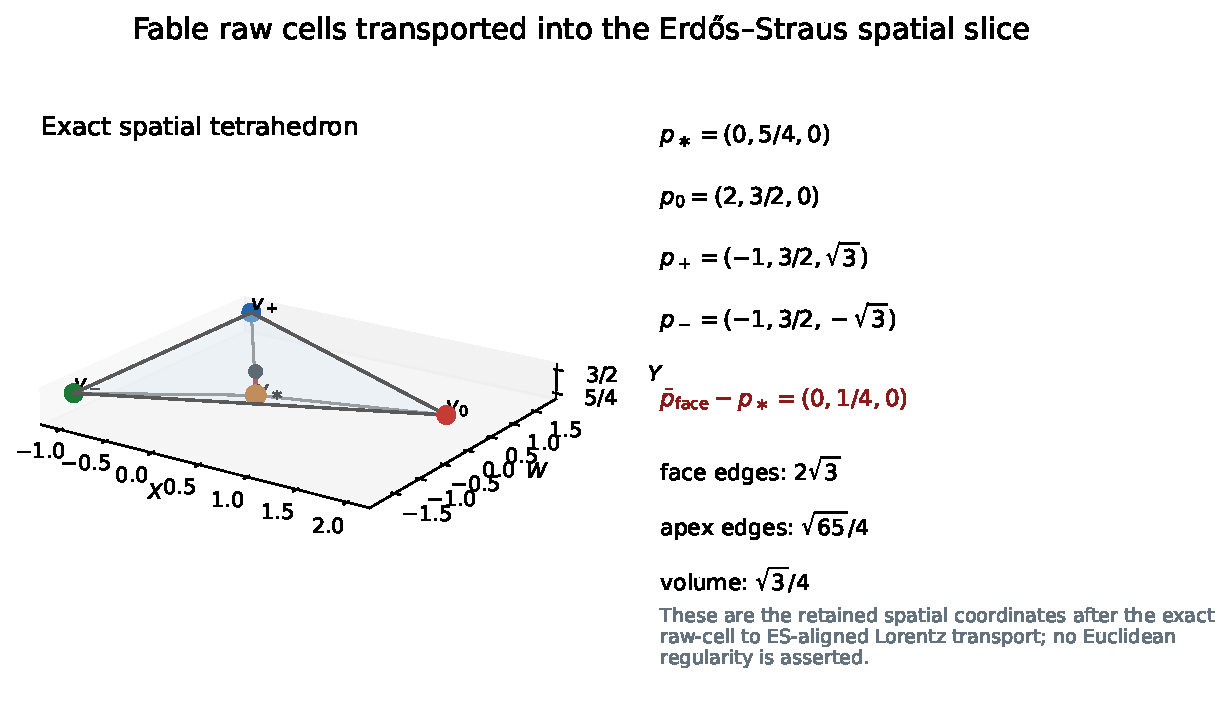
\includegraphics[width=.96\textwidth]{figures/fable-es-raw-tetrahedron-3d.pdf}
\caption{The actual spatial projection in EZ35B--EZ35D.  The three null
vertices lie in the plane \(Y=3/2\); the spacelike apex lies at \(Y=5/4\).
The face centroid and apex have identical \(X,W\) coordinates and differ by
the exact quarter.  Axis coordinates and all metric quantities are retained;
the drawing does not assert Euclidean regularity.  The figure source is
\texttt{tools/generate\_20260920\_illustrations.py}; the exact coordinate
certificate is the local
\texttt{verify\_fable\_es\_raw\_tetrahedron.py}, reproduced from the cited
canonical source calculation.}
\label{fig:fable-es-raw-tetrahedron}
\end{figure}


\section{The odd receiving divisor pulled back to the Erd\H{o}s--Straus locus}
\label{sec:odd-receiver-pullback}

This section applies the odd receiving-frame calculation of the fixed
weighted-conductor source to the literal Erd\H{o}s--Straus coefficient map.
The nonlinear Fable map, the invertible linear conductor, and the odd receiving
matrix are three different maps.  Only the third map is considered here.
The inverse branches and their original source coordinates are those of
\cite[GF5--GF12]{SignedCover}; the determinant divisor and its ES pullback are
calculated below.

For a target \(u=(A,B,C,D)\), put
\[
 h_u(r)=Ar^4+r^3+Br^2+Cr+D,
 \qquad d(r)=h_u'(r).
\]
On the open locus where \(A\ne0\) and \(h_u\) has four distinct roots
\(r_1,\ldots,r_4\), choose \(\xi_j\) with
\(\xi_j^2d(r_j)=1\).  The odd columns of the eight signed inverse states are
\begin{equation}
 o_j=\xi_j
 \begin{pmatrix}
  1\\ -\ii d(r_j)\\ A d(r_j)^2+2r_jd(r_j)\\
  \ii\bigl(7r_j^2d(r_j)-13d(r_j)^2\bigr)
 \end{pmatrix},
 \qquad O=[o_1\ \cdots\ o_4].                         \tag{EZ37}
\end{equation}
Changing an individual square-root sign changes the corresponding column sign;
therefore the determinant zero locus is independent of these choices.

\begin{proposition}[Exact odd receiving divisor]
\label{prop:odd-divisor}
Define
\begin{align}
 \mathfrak D_{\rm odd}(A,B,C,D)
 :={}&20(3C-B^2)+A(87B^3-282BC-51D)\nonumber\\
 &+A^2(-28B^4+22B^2C+431C^2+204BD)\nonumber\\
 &+A^3(224B^2D-168BC^2-856CD)-448A^4D^2.       \tag{EZ38}
\end{align}
Then
\begin{equation}
 \det O=\varepsilon_{\rm br}\,
 \frac{4\mathfrak D_{\rm odd}(A,B,C,D)}{A^3},
 \qquad \varepsilon_{\rm br}\in\{1,-1\}.             \tag{EZ39}
\end{equation}
\end{proposition}

\begin{proof}
Reduce the four component polynomials in EZ37 modulo \(h_u\) in the ordered
basis \(1,r,r^2,r^3\).  The first reduced polynomial is \(1\).  Removing its
row and column leaves the coefficient matrix
\[
\mathsf R=
\begin{pmatrix}
2B&3&4A\\
4ABC-8AD-7C&4AB^2-2AC-16A^2D-5B&4AB-8A^2C-3\\
20C/A+76D-52BC&20B/A+5C-52B^2+208AD&20/A-66B+104AC
\end{pmatrix}.
\]
Direct expansion, without changing coordinates, gives
\(\det\mathsf R=4\mathfrak D_{\rm odd}/A\).  Let
\(V=\prod_{j<k}(r_k-r_j)\).  Since
\[
 \prod_jd(r_j)=A^4V^2,
 \qquad
 \left(V\prod_j\xi_j\right)^2=A^{-4},
\]
one has \(V\prod_j\xi_j=\varepsilon_{\rm br}A^{-2}\).  Multiplying the
coefficient determinant, the evaluation Vandermonde and the four retained
square-root factors proves EZ39.
\end{proof}

Return to the ordered Erd\H{o}s--Straus source EZ1--EZ3.  For compactness write
\begin{equation}
 S=p+s_1,\qquad b=ps_1+s_2,\qquad c=ps_2+s_3,\qquad d=ps_3.       \tag{EZ40}
\end{equation}
The normalized coefficient map EZ7 is
\begin{equation}
 \Theta(p,s_1,s_2,s_3)
 =\left(-\frac1S,-\frac bS,\frac cS,-\frac dS\right).           \tag{EZ41}
\end{equation}
Its domain in this section is the ordered algebraic ES source
\[
 X_{\rm ES}^{\rm ord}
 =\{ps_2=4s_3,\;Sps_3\Delta\ne0\},
\]
where \(\Delta\) is the discriminant of the four literal roots.  The codomain
of \(\Theta\) is the coefficient affine space \(\mathbb A^4_{A,B,C,D}\), and
\(\mathfrak D_{\rm odd}:\mathbb A^4\to\mathbb A^1\).

\begin{theorem}[Exact pullback and scale-free irreducible divisor]
\label{thm:odd-pullback}
The composite \(\mathfrak D_{\rm odd}\circ\Theta\) is
\begin{equation}
 \mathfrak D_{\rm odd}\circ\Theta=\frac{\widetilde P}{S^6},     \tag{EZ42}
\end{equation}
where
\begin{align*}
\widetilde P={}&60cS^5-(20b^2+51d)S^4-282bcS^3\\
&+(87b^3+431c^2+204bd)S^2+(22b^2c-856cd)S\\
&-28b^4+224b^2d-168bc^2-448d^2.
\end{align*}
On the ES relation, put
\begin{equation}
 T=\frac{s_1}{p},\qquad Z=\frac{s_3}{p^3}.                       \tag{EZ43}
\end{equation}
Then
\begin{equation}
 \mathfrak D_{\rm odd}\circ\Theta
 =\frac{p^2\Phi(T,Z)}{(1+T)^6},                                  \tag{EZ44}
\end{equation}
with
\begin{align}
\Phi(T,Z)={}&-7168Z^4+32(174T^2+179T-184)Z^3\nonumber\\
&+(-320T^4-2744T^3-705T^2+3350T+903)Z^2\nonumber\\
&+(140T^5+443T^4-440T^3-390T^2-70T+249)Z\nonumber\\
&-T^2(T-1)^2(20T^2+33T+20).                              \tag{EZ45}
\end{align}
The polynomial \(\Phi\) is primitive and irreducible over \(\Q\).
\end{theorem}

\begin{proof}
Substitution of EZ41 into every retained term of EZ38 and collection over the
common denominator \(S^6\) gives EZ42.  On \(ps_2=4s_3\), the quantities in
EZ40 become
\[
 S=p(1+T),\qquad b=p^2(T+4Z),\qquad c=5p^3Z,\qquad d=p^4Z.
\]
Substitution into EZ42 and collection of the factor \(p^2/(1+T)^6\) gives
EZ44--EZ45 term for term.  The exact checker factors \(\Phi\) independently
with SymPy and python-flint.  Both return a single primitive factor.  Its
reduction modulo \(11\) is again one degree-six factor, so Gauss's lemma also
certifies irreducibility over \(\Q\).
\end{proof}

The supplied coefficient point from the receiving-frame calculation is not on
the ES coefficient hypersurface.  Indeed, for
\(u_*=(1,0,-60/431,0)\), the polynomial \(G\) of EZ9 gives
\begin{equation}
 G(u_*)=-\frac{51840000}{34507149121}\ne0.                        \tag{EZ46}
\end{equation}
It also has \(A>0,D=0\), whereas every positive ES image in EZ7 has
\(A<0,D<0\).  This proves a specific nonidentity; it does not make the two
divisors unrelated, because EZ42--EZ45 are their exact pullback relation.

\begin{theorem}[Positive-real intersection and exact arithmetic residue]
\label{thm:odd-positive-real}
The divisor \(V(\Phi)\) meets the positive-real, pairwise-distinct ES locus.
More precisely, set \(p=1\) and
\begin{equation}
 \frac px=\frac14-\delta,\qquad
 \frac py=\frac14+\delta,\qquad
 \frac pz=\frac72,                                                \tag{EZ47}
\end{equation}
where \(w=\delta^2\).  Then \(4/p=1/x+1/y+1/z\), and
\[
 \mathfrak D_{\rm odd}\circ\Theta
 =-\frac{8Q(w)}{(144w-65)^6},
\]
where
\begin{align*}
Q(w)={}&319186534400w^6+12383961481216w^5-26262983737344w^4\\
&-1257389244416w^3+1383887871744w^2
+2670303991200w-90309375.
\end{align*}
One has \(Q(10^{-6})<0<Q(10^{-4})\).  Consequently some
\(w_0\in(10^{-6},10^{-4})\) gives a positive, pairwise-distinct real ES point
on the divisor.

For positive rational ES shapes, intersection with this divisor is exactly the
following splitting problem:
\begin{equation}
\begin{gathered}
 \Phi(T,Z)=0,\\
 X^3-TX^2+4ZX-Z
 \text{ splits into three distinct positive rational roots,}\\
 \text{none equal to }1.
\end{gathered}                                                       \tag{EZ48}
\end{equation}
If the three roots in EZ48, written in lowest terms, have common denominator
\(L\), the shape lifts to a positive integral ES solution at every positive
integer scale \(p\) divisible by \(L\).  It lifts with \(p\) prime exactly when
\(L=1\) or \(L\) itself is prime.  No existence or nonexistence result for
such a prime-integral point is asserted here.
\end{theorem}

\begin{proof}
The three reciprocals in EZ47 sum to \(4\).  For
\(10^{-6}<w<10^{-4}\), one has \(0<\delta<1/100\), so all three are positive
and distinct.  Direct substitution into EZ38 gives the displayed rational
function.  Its denominator is positive on the closed interval and the exact
endpoint numerators are
\[
 Q(10^{-6})=
 -\frac{208947824537547554186600178130584239}
 {2384185791015625000000000000}<0,
\]
\[
 Q(10^{-4})=
 \frac{421368746134524395585536}{2384185791015625}>0.
\]
The intermediate value theorem proves the real intersection.

For the arithmetic statement, the roots of the cubic in EZ48 are precisely
\(x/p,y/p,z/p\): their first and third elementary symmetric functions are
\(T=s_1/p\) and \(Z=s_3/p^3\), while EZ3 gives the middle elementary symmetric
function \(s_2/p^2=4Z\).  Positive integral denominators give the stated
rational splitting.  Conversely, if \(L\) is the least common denominator of
the three roots, every multiple \(p\) of \(L\) makes \(x,y,z\) integral, and
\(s_2/p^2=4s_3/p^3\) gives the ES equation.  Such a multiple can be prime
exactly when \(L=1\), in which case any prime works, or \(L\) is prime, in
which case the only prime multiple is \(p=L\).  Distinctness and exclusion of
the root \(1\) are exactly the retained root-collision and
prime-equals-denominator exclusions.  This proves every assertion.
\end{proof}

\begin{figure}[htbp]
\centering
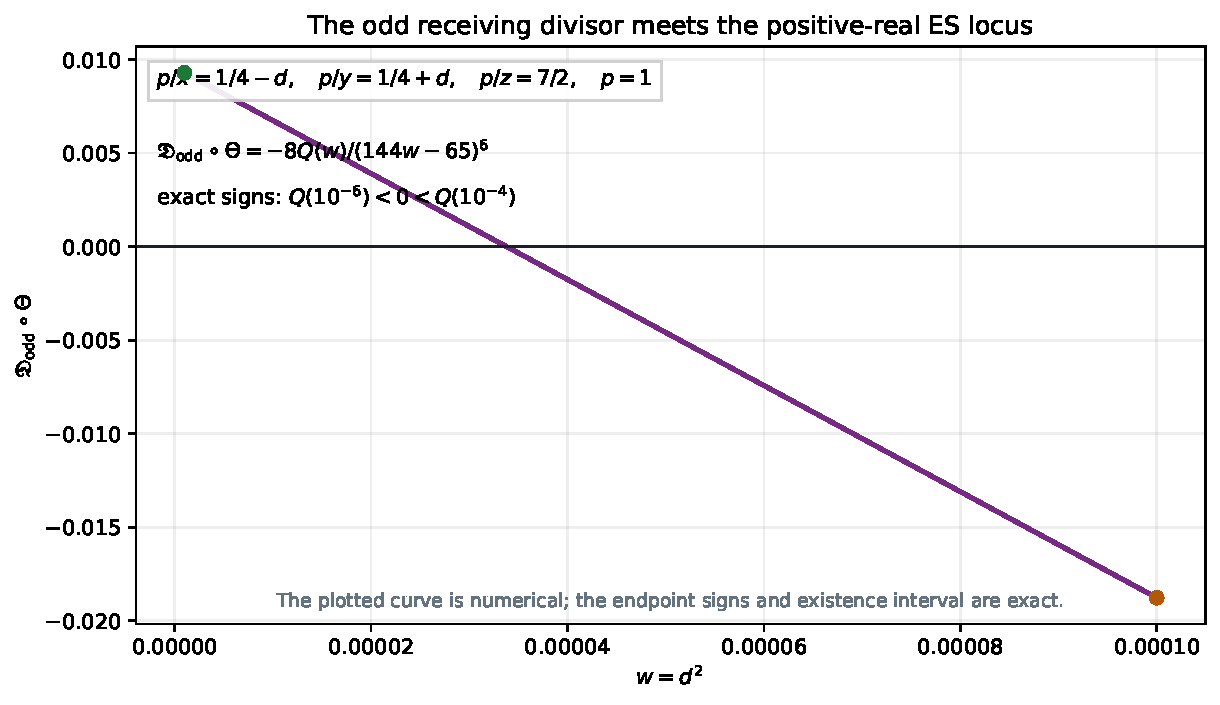
\includegraphics[width=.93\textwidth]{figures/odd-receiver-positive-real-crossing.pdf}
\caption{The exact one-parameter section EZ47 of the positive-real ES locus.
The curve is rendered numerically, while the two endpoint signs printed in
the proof are exact rational inequalities.  Their sign change proves an
intersection with the receiving divisor; it does not prove a rational or
integral intersection.  Reproduce with
\texttt{tools/generate\_20260920\_illustrations.py} and certify with
\texttt{verify\_odd\_receiver\_es\_pullback.py}.}
\label{fig:odd-receiver-positive-real-crossing}
\end{figure}


\section{Every hard-prime witness lies in the eight-sheet domain}
\label{sec:hard-prime-domain}

The earlier exterior-state theorem can be strengthened without an exterior
channel hypothesis.  Throughout this section \(p\) is a positive prime with
\(p\equiv1\pmod {12}\), and

\begin{equation}
 \frac4p=\frac1x+\frac1y+\frac1z,
 \qquad x,y,z\in\mathbb Z_{>0}.                       \tag{EZ49}
\end{equation}

\begin{theorem}[Distinctness of every hard-prime witness]
\label{thm:hard-prime-distinct}
The four integers \(p,x,y,z\) in EZ49 are pairwise distinct.  Consequently
the normalized literal-root quartic EZ6 has nonzero discriminant, and its
Fable inverse has eight distinct signed states.
\end{theorem}

\begin{proof}
If one denominator equals \(p\), relabel it as \(x=p\).  Then

\[
 \frac3p=\frac1y+\frac1z,
 \qquad (3y-p)(3z-p)=p^2.
\]

Positivity of the reciprocal equation gives \(y,z>p/3\), so both factors are
positive integers.  Since \(p\) is prime, each factor belongs to
\(\{1,p,p^2\}\).  Every element of this set is \(1\pmod3\), because
\(p\equiv1\pmod3\), whereas \(3y-p\equiv2\pmod3\).  This is impossible.

If two denominators coincide, relabel them as \(x=y=a\).  Positivity gives
\(a>p/2\).  Put \(d=2a-p>0\).  Exact rearrangement of EZ49 gives

\[
 4dz=p(d+p),
\]

so \(d\mid p^2\).  The three possibilities \(d=1,p,p^2\) give, respectively,

\[
 z=\frac{p(p+1)}4,\qquad z=\frac p2,\qquad z=\frac{p+1}4.
\]

None is integral when \(p\equiv1\pmod4\).  Symmetry excludes every collision
of these two types.  Thus all four literal roots are distinct.  At every
simple root \(t\), the equation \(\xi^2h_u'(t)=1\) has two nonzero solutions;
the root and the sign distinguish the resulting eight source points.
\end{proof}

\begin{theorem}[Fixed-input separation and inverse bounds]
\label{thm:hard-prime-bounds}
Relabel the denominators so that \(x<y<z\), and define

\begin{equation}
 R=4x-p,\qquad S_R=px=\frac{p(p+R)}4,\qquad
 s_p=\frac{p(p+3)}4,\qquad
 B_p=p+s_p(s_p+1).                                   \tag{EZ50}
\end{equation}

Then

\begin{equation}
 \frac p4<x<\frac{3p}4,\qquad 3\le R\le2p-3,          \tag{EZ51}
\end{equation}

and

\begin{equation}
 (Ry-S_R)(Rz-S_R)=S_R^2,\qquad
 z\le\frac{s_p(s_p+1)}3,\qquad
 S=p+x+y+z\le B_p.                                   \tag{EZ52}
\end{equation}

For \(t_1,t_2,t_3,t_4=p,x,y,z\),

\begin{equation}
 \boxed{\Disc(h_u)
 =S^{-6}\prod_{j<k}(t_j-t_k)^2
 \ge\frac{144}{B_p^6}.}                              \tag{EZ53}
\end{equation}

At every selected root \(t_j\),

\begin{equation}
 \frac2S\le |h_u'(t_j)|\le S^2,\qquad
 \frac1S\le|\xi_j|\le\sqrt{\frac S2}.                \tag{EZ54}
\end{equation}

The complete inverse point \(q_j=(\xi_j,y_j,z_j,w_j)\), with the coordinates
of EZ13 retained, satisfies

\begin{equation}
 |y_j|\le2S,\qquad |z_j|\le6S^2,\qquad |w_j|\le41S^3. \tag{EZ55}
\end{equation}

If \(G\) is any specified positive-definite Hermitian Gram matrix in these
four source coordinates and \(\|G\|_2\) is its spectral norm, then

\begin{equation}
 \boxed{
 \|q_j\|_G^2\le\|G\|_2
 \left(\frac S2+4S^2+36S^4+1681S^6\right).}          \tag{EZ56}
\end{equation}
Every right-hand side can be made a function of \(p\) alone by replacing
\(S\) with \(B_p\); the lower bounds become \(2/B_p\) and \(1/B_p\).
\end{theorem}

\begin{proof}
Since \(x\) is the smallest denominator,
\(1/x<4/p<3/x\), which proves the first inequalities in EZ51.  Because
\(p\equiv1\pmod4\), the positive integer \(R=4x-p\) is \(3\pmod4\).
The strict upper bound on \(x\) then gives \(3\le R\le2p-3\).

The remaining two reciprocals satisfy

\[
 \frac1y+\frac1z=\frac{R}{S_R}.
\]

Multiplication gives the first identity in EZ52.  Both factors on its left
are positive: each of \(1/y\) and \(1/z\) is strictly smaller than their sum
\(R/S_R\).  Hence \(Rz-S_R\le S_R^2\), and

\[
 z\le\frac{S_R(S_R+1)}R.
\]

The following subtraction is exact:

\[
 \frac{S_R(S_R+1)}R-\frac{s_p(s_p+1)}3
 =\frac{p^2(R-3)}{16}
   \left(1-\frac{p^2+4}{3R}\right).
\]

It is nonpositive on EZ51 because

\[
 p^2+4-3R\ge p^2+4-3(2p-3)=(p-3)^2+4>0.
\]

This proves the bound on \(z\).  Since \(x+y+z\le3z\), it also proves
\(S\le B_p\).

For four ordered distinct integers, their six positive pairwise gaps are at
least \(1,1,1,2,2,3\); their product is at least \(12\).  The normalized
leading coefficient is \(-S^{-1}\), so the quartic discriminant is the first
expression in EZ53 and the asserted lower bound follows.

At a root,

\[
 h_u'(t_j)=-S^{-1}\prod_{\ell\ne j}(t_j-t_\ell).
\]

The three signed differences are distinct nonzero integers, and their
absolute product is at least \(2\).  Each absolute difference is smaller
than \(S\).  This proves the derivative bounds.  Taking absolute values in
\(\xi_j^2h_u'(t_j)=1\) proves the bounds on \(\xi_j\).

Put \(v=|\xi_j|^{-1}\le S\) and \(t=t_j\le S\).  The literal coefficient
bounds are \(|A|=S^{-1}\) and \(|B|<S\).  Applying them term by term to EZ13
gives

\[
 |y_j|\le t+v\le2S,
\]

\[
 |z_j|\le |A|v^3+2tv+3v^2\le6S^2,
\]

and

\[
 |w_j|\le7t^2v+(|B|+17t+|A|t^2)v^2+13v^3+2|A|v^4
 \le41S^3.
\]

Finally \(q_j^*Gq_j\le\|G\|_2\|q_j\|_2^2\), and EZ54--55 give EZ56.
\end{proof}

The preceding theorem is a compactness statement only after \(p\) has been
fixed.  Its bounds grow with \(p\), and it neither proves that a witness exists
nor bounds the separate odd receiving divisor away from zero.

\section{The fixed-input signed cover}
\label{sec:fixed-input-cover}

Fix \(p\in\mathbb C^\times\).  On the coefficient hypersurface, retain both
the intrinsic-root relation \(p=-5D/C\) and EZ9.  On \(ACD\ne0\), these two
relations are equivalent to

\begin{equation}
 D=-\frac{pC}{5},\qquad
 B=-Ap^2-p-\frac{4C}{5p}.                             \tag{EZ57}
\end{equation}

Substitution gives

\begin{equation}
 h_u(r)=(r-p)g_p(r),\qquad
 g_p(r)=Ar^3+(1+Ap)r^2-\frac{4C}{5p}r+\frac C5,       \tag{EZ58}
\end{equation}

and

\begin{equation}
 d_p=g_p(p)=2Ap^3+p^2-\frac{3C}{5},\qquad
 \Disc(h_u)=d_p^2\Disc(g_p).                         \tag{EZ59}
\end{equation}

Let

\[
 \mathcal B_p=\{(A,C):A C d_p\Disc(g_p)\ne0\},
\]

and let \(\mathcal R_p\) be its coordinate ring.  The factor \(C\) is retained
because this is the intrinsic-prime ES chart.  The exact squarefreeness
boundary at fixed \(p\ne0\) is \(A d_p\Disc(g_p)=0\).

\begin{theorem}[Rank \(2+6\) decomposition]
\label{thm:fixed-input-split}
In \(\mathcal R_p[r]/(h_u)\),

\begin{equation}
 e_p(r)=\frac{g_p(r)}{d_p}                            \tag{EZ60}
\end{equation}

is the idempotent equal to one at the marked root \(p\) and zero at the three
denominator roots.  The signed inverse algebra splits as

\begin{equation}
\boxed{
\begin{aligned}
 \mathcal S_p\simeq{}&
 \mathcal R_p[\xi]/(\xi^2d_p-1)\\
 &\times
 \left(\mathcal R_p[r]/(g_p)\right)[\xi]
 \big/\left(\xi^2(r-p)g_p'(r)-1\right).
\end{aligned}}                                      \tag{EZ61}
\end{equation}

The two factors have ranks two and six over \(\mathcal R_p\).
\end{theorem}

\begin{proof}
Substituting the first identity of EZ57 into EZ9 gives

\[
 -C^3(5Ap^3+5p^2+5pB+4C)=0,
\]

which gives the second identity of EZ57 because \(pC\ne0\).  Direct
multiplication proves EZ58.  The resultant product formula gives EZ59.
Chinese remaindering by the coprime factors \(r-p\) and \(g_p\) gives the
idempotent EZ60.  Finally

\[
 h_u'(p)=d_p,\qquad h_u'(r)=(r-p)g_p'(r)\quad\text{on }g_p(r)=0,
\]

and substituting these identities into \(\xi^2h_u'(r)=1\) proves EZ61.
\end{proof}

\begin{theorem}[Order-\(48\) monodromy and exact deck group]
\label{thm:fixed-input-monodromy}
Label the marked root by \(0\) and the denominator roots by \(1,2,3\).  The
monodromy image on the eight signed states over \(\mathcal B_p\) is

\begin{equation}
 \boxed{
 G_p=\left\{(\sigma,\pi)\in\{\pm1\}^4\rtimes S_4:
 \pi(0)=0,
 \ \prod_{j=0}^3\sigma_j=\operatorname{sgn}(\pi)\right\},}
 \qquad |G_p|=48.                                    \tag{EZ62}
\end{equation}

The deck group of the disconnected rank-\(2+6\) cover is

\begin{equation}
 \boxed{\operatorname{Deck}(\mathcal S_p/\mathcal B_p)
 \simeq C_2\times C_2.}                              \tag{EZ63}
\end{equation}
\end{theorem}

\begin{proof}
Let \(\Delta=\prod_{j<k}(t_k-t_j)\).  Since

\[
 \prod_jh_u'(t_j)=A^4\Delta^2,
\]

the retained signed invariant

\[
 \chi=A^2\Delta\prod_j\xi_j\in\{1,-1\}
\]

is locally constant.  Continuation by \((\sigma,\pi)\) therefore forces
\(\prod_j\sigma_j=\operatorname{sgn}(\pi)\).  The marked root cannot move,
which proves the upper bound in EZ62.

Define the ordered denominator space \(X_p\) by choosing \((x,y)\in\mathbb
C^2\), putting

\begin{equation}
 z=\frac{pxy}{4xy-p(x+y)},                            \tag{EZ64}
\end{equation}

and deleting the loci on which a denominator is zero, two of
\(p,x,y,z\) collide, the denominator in EZ64 vanishes, or
\(S=p+x+y+z\) vanishes.  This is the complement of finitely many complex
algebraic curves in \(\mathbb C^2\), and it is nonempty.  It is also path
connected.  Given two retained points, the complex affine line through them
cannot be contained in any deleted curve, because both endpoints lie outside
that curve.  It therefore meets each deleted algebraic curve in finitely many
points.  A complex line with finitely many points removed is path connected,
so the two retained points are joined inside \(X_p\).

There is an exact coefficient map

\[
 q_p:X_p\longrightarrow\mathcal B_p,
 \qquad
 q_p(x,y)=\left(-\frac1{p+x+y+z},
                 \frac{5xyz}{p+x+y+z}\right)=(A,C).
\]

It is invariant under all six reorderings of \((x,y,z)\).  The reciprocal
equation and the two displayed coefficients give the literal identity

\[
 A\prod_{t\in\{p,x,y,z\}}(r-t)=(r-p)g_p(r).
\]

The deletions in the definition of \(X_p\) then give
\(ACd_p\Disc(g_p)\ne0\), so \(q_p\) lands in \(\mathcal B_p\).
Conversely, for
\((A,C)\in\mathcal B_p\), the unordered denominator triple is exactly the
root set of

\[
 \frac{g_p(r)}A
 =r^3+\left(p+\frac1A\right)r^2
   -\frac{4C}{5pA}r+\frac{C}{5A}.
\]

Thus its elementary symmetric functions are

\[
 x+y+z=-p-\frac1A,\qquad
 xy+xz+yz=-\frac{4C}{5pA},\qquad
 xyz=-\frac{C}{5A}.
\]

They obey \(p(xy+xz+yz)=4xyz\), which is precisely the reciprocal
Erd\H{o}s--Straus equation and gives EZ64.  The factors defining
\(\mathcal B_p\) say exactly that these roots are nonzero, mutually distinct,
different from \(p\), and have \(S\ne0\).  Hence every fibre of \(q_p\) is
the free six-element ordering orbit, and the elementary-symmetric inverse
proves the exact quotient

\[
 X_p/S_3\;\xrightarrow{\ \sim\ }\;\mathcal B_p.
\]

Since \(X_p\) is connected, this finite \(S_3\)-cover has unsigned monodromy
equal to all of \(S_3\).

The sign subgroup is realized by two exact local families.  First put

\[
 x=p(2+w),\qquad y=p(2-w),\qquad
 z=p\frac{4-w^2}{12-4w^2}.
\]

For \(0<|w|\le1/10\), only \(x=y\) occurs inside the puncture.  The two
coefficient and derivative factors are

\[
 A=-\frac{4(w^2-3)}{p(21w^2-64)},\qquad
 C=-\frac{5p^2(w-2)^2(w+2)^2}{21w^2-64},
\]

\[
 h_u'(p)=
 \frac{p^2(w-1)(w+1)(3w^2-8)}{21w^2-64},
\]

\[
 h_u'(x)=
 -\frac{2p^2w(w+1)(w+2)(4w^2-w-10)}{21w^2-64},
\]

\[
 h_u'(y)=
 \frac{2p^2w(w-2)(w-1)(4w^2+w-10)}{21w^2-64}.
\]

\[
 h_u'(z)=
 -\frac{p^2(w-2)(w+2)(3w^2-8)
 (4w^2-w-10)(4w^2+w-10)}
 {16(w^2-3)^2(21w^2-64)}.
\]

On \(|w|\le1/10\), the estimates
\(|21w^2|<64\), \(|3w^2|<8\), and
\(|4w^2\mathbin{\pm}w|<10\), together with
\(|w|<1<2\), prove that every displayed base factor and every derivative
factor other than the single \(w\)-factor in \(h_u'(x),h_u'(y)\) is nonzero.
Thus the path stays in \(\mathcal B_p\) away from its central collision.  A
half-circle exchanges \(x,y\); its square fixes the labels and flips exactly
their two square-root signs.

Next put

\[
 x=p(1+w),\qquad y=\frac{2p}{5},\qquad
 z=\frac{2p(1+w)}{1+3w}.
\]

For \(0<|w|\le1/100\), only \(p=x\) occurs inside the puncture, and

\[
 A=-\frac{5(3w+1)}{p(15w^2+51w+22)},\qquad
 C=\frac{20p^2(w+1)^2}{15w^2+51w+22},
\]

\[
 h_u'(p)=\frac{3p^2w(w-1)}{15w^2+51w+22},
\]

\[
 h_u'(x)=
 -\frac{p^2w(w+1)(3w-1)(5w+3)}{15w^2+51w+22}.
\]

\[
 h_u'(y)=
 \frac{12p^2(w+2)(5w+3)}{25(15w^2+51w+22)},
\]

\[
 h_u'(z)=
 -\frac{4p^2(w-1)(w+1)(w+2)(3w-1)}
 {(3w+1)^2(15w^2+51w+22)}.
\]

For \(|w|\le1/100\),
\(|15w^2+51w|<22\); all remaining displayed linear factors are separated
from zero except the single \(w\)-factor in \(h_u'(p),h_u'(x)\).  Hence this
path also stays in \(\mathcal B_p\) away from its central collision.  A full circle fixes every root
label and flips exactly the signs over \(p,x\).  Denominator pair flips span
the even-sign plane on the three denominator labels; adjoining this
prime--denominator flip spans all eight even sign vectors.  With the six
denominator permutations, the realized image has \(8\cdot6=48\) elements and
attains the upper bound.

The two connected sheet-orbits have sizes two and six.  On the six
denominator sheets, the induced action is the full signed permutation group
\(C_2^3\rtimes S_3\), whose centralizer is generated by simultaneous
denominator sign reversal.  The prime-pair centralizer is \(C_2\).  The two
deck maps can be written

\[
 \xi\longmapsto(1-2e_p)\xi,\qquad \xi\longmapsto-\xi.
\]

They independently reverse the prime pair and the denominator sheets, and
their products exhaust the centralizer.  This proves EZ63.
\end{proof}

\begin{corollary}[Correct order-\(48\) orbit metric]
\label{cor:fixed-input-metric}
In even/odd coordinates for each signed root pair, the eight-dimensional
representation is

\begin{equation}
 \mathbf1^{\oplus2}\oplus V_2\oplus\chi_{\det}\oplus V_3,       \tag{EZ65}
\end{equation}

where \(V_2\) is the standard two-dimensional \(S_3\)-module,
\(V_3\) is the three-dimensional signed-permutation module, and

\[
 \chi_{\det}(\sigma,\pi)
 =\operatorname{sgn}(\pi)\prod_{i=1}^3\sigma_i=\sigma_0.
\]

Let \(E=[e_p,E_d]\) and \(O=[o_p,O_d]\) be the original even and odd source
columns, and let \(G\) be the specified receiving form.  Averaging the pulled
back Gram matrix over \(G_p\), in the corresponding orthonormal decomposition,
gives

\begin{equation}
 \boxed{H_{\rm triv}\oplus\lambda_2I_2\oplus\lambda_p
 \oplus\lambda_3I_3,}                                \tag{EZ66}
\end{equation}

where

\[
 H_{\rm triv}=
 \begin{bmatrix}e_p&E_d\mathbf1/\sqrt3\end{bmatrix}^{*}G
 \begin{bmatrix}e_p&E_d\mathbf1/\sqrt3\end{bmatrix},
\]

\[
 \lambda_2=\frac12\operatorname{tr}(P_2E_d^*GE_d),
 \quad P_2=I_3-\frac13\mathbf1\mathbf1^*,
 \quad\lambda_p=o_p^*Go_p,
 \quad\lambda_3=\frac13\operatorname{tr}(O_d^*GO_d).
\]

In particular, the mutual Gram term between the prime-even state and the
denominator-even sum survives; the two-dimensional block cannot be replaced
by two unrelated scalars.
\end{corollary}

\begin{proof}
The even denominator permutation module is
\(\mathbf1\oplus V_2\), while the prime-even line is another trivial module.
The prime-odd line transforms by \(\chi_{\det}\), and the three denominator-odd
coordinates form \(V_3\).  Averaging kills maps between inequivalent
summands, retains the full Gram form on the two equivalent trivial copies,
and gives the normalized traces on the irreducible \(V_2,V_3\) blocks.  The
one-dimensional \(\chi_{\det}\) block is \(o_p^*Go_p\).  These are exactly the
four blocks in EZ66.
\end{proof}

\begin{figure}[htbp]
\centering
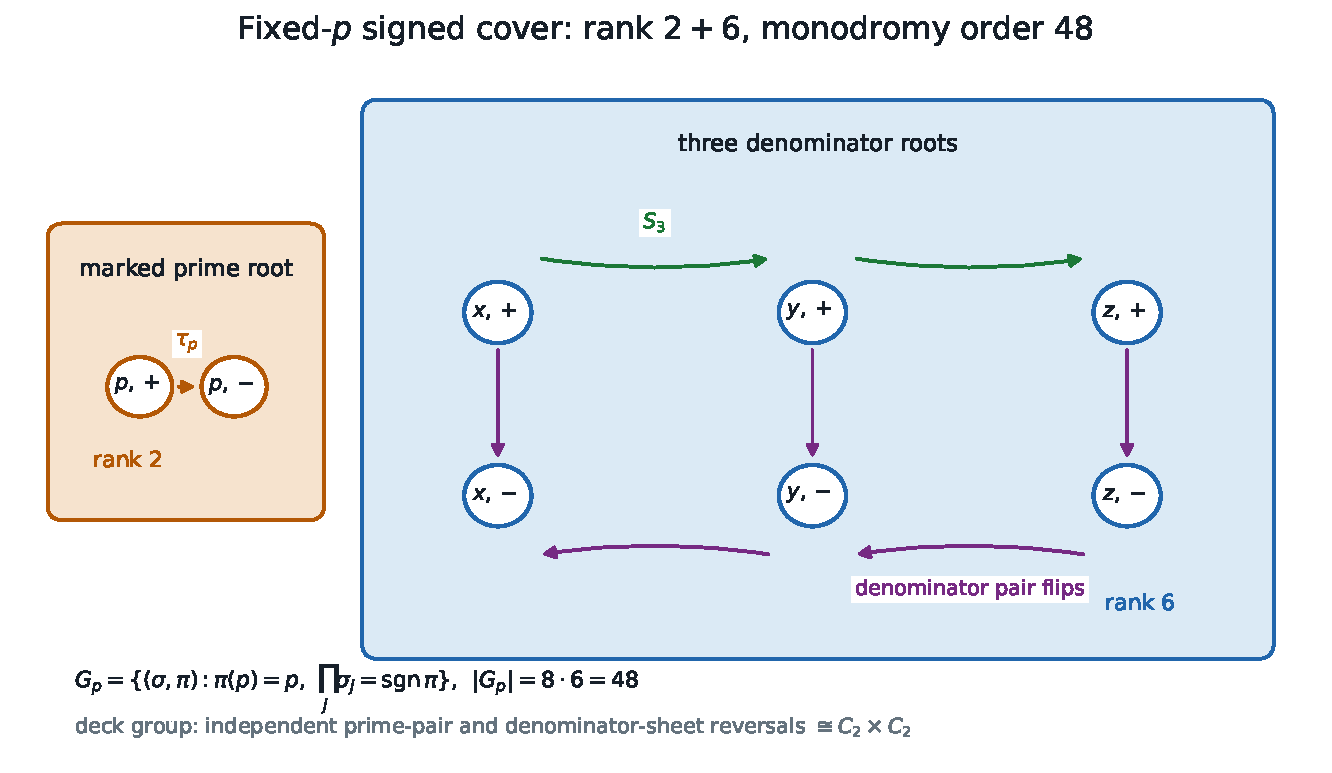
\includegraphics[width=.94\textwidth]{figures/fixed-input-cover-decomposition.pdf}
\caption{The proved fixed-input decomposition.  The marked prime produces a
rank-two component and the three denominator roots a rank-six component.
Denominator permutations, denominator pair flips, and one
prime--denominator flip generate the order-\(48\) monodromy; the two displayed
deck reversals commute with it.  This is a sheet-action diagram, not a metric
embedding.  Reproduce it with
\texttt{tools/generate\_20260920\_illustrations.py}; exact group enumeration
is in \texttt{verify\_fixed\_input\_boundary.py}.}
\label{fig:fixed-input-cover}
\end{figure}

\section{Finite completion of the inverse-derivative boundary}
\label{sec:finite-completion}

Work over

\[
 \mathcal R_0=\mathbb C[A,A^{-1},B,C,D],\qquad
 \mathcal E=\mathcal R_0[r]/(h_u).
\]

Introduce the reciprocal signed coordinate \(\eta=\xi^{-1}\) and define

\begin{equation}
 \boxed{\widehat{\mathcal S}
 =\mathcal E[\eta]/(\eta^2-h_u'(r)).}                 \tag{EZ67}
\end{equation}

\begin{theorem}[Finite flat rank-eight completion]
\label{thm:finite-completion}
The algebra EZ67 is free of rank eight over \(\mathcal R_0\), with basis

\begin{equation}
 1,r,r^2,r^3,\eta,\eta r,\eta r^2,\eta r^3.           \tag{EZ68}
\end{equation}

It recovers the original signed inverse exactly on \(\eta\ne0\):

\begin{equation}
 \boxed{
 \mathcal E[\xi]/(\xi^2h_u'-1)
 \simeq\widehat{\mathcal S}[\eta^{-1}],\qquad
 \eta=\xi h_u'=\xi^{-1},\quad \xi=\eta^{-1}.}         \tag{EZ69}
\end{equation}

Thus its spectrum is finite flat of degree eight and proper over
\(\operatorname{Spec}\mathcal R_0\).  Its ramification Jacobian in the
\((r,\eta)\) variables is

\begin{equation}
 \det
 \begin{pmatrix}h_u'(r)&0\\-h_u''(r)&2\eta\end{pmatrix}
 =2\eta h_u'(r)=2\eta^3.                              \tag{EZ70}
\end{equation}
\end{theorem}

\begin{proof}
Because \(A\) is a unit, \(A^{-1}h_u\) is monic of degree four; hence
\(\mathcal E\) is free of rank four.  The relation in EZ67 is monic of degree
two in \(\eta\), which proves EZ68.  Inverting \(\eta\) and setting
\(\xi=\eta^{-1}\) gives \(\xi^2h_u'=1\).  Conversely, in the original signed
algebra, \(\eta=\xi h_u'\) is the inverse of \(\xi\) and satisfies
\(\eta^2=h_u'\).  This proves EZ69.  A finite morphism is proper
\cite{StacksFinite}.  Direct differentiation gives EZ70; away from
\(\eta=0\), its determinant is a unit, agreeing with the standard
derivative-unit criterion for an étale algebra \cite{StacksEtale}.
\end{proof}

The completion is over \(A\ne0\).  It does not repair the independent
infinity-chart boundary \(A=0\).

\begin{proposition}[The original meromorphic pole is retained]
\label{prop:retained-pole}
In the completed coordinates, the original inverse point is

\begin{equation}
 q=\begin{pmatrix}
 \eta^{-1}\\
 -r-\ii\eta\\
 A\eta^3+2r\eta+3\ii\eta^2\\
 7\ii r^2\eta+(B-17r+Ar^2)\eta^2-13\ii\eta^3-2A\eta^4
 \end{pmatrix}.                                      \tag{EZ71}
\end{equation}

Let a path approach a fixed finite coefficient target of
\(\operatorname{Spec}\mathcal R_0\), with \(\eta\to0\); equivalently the
coefficients and \(r\) remain bounded and \(A\) stays nonzero.  For any fixed
injective receiving map \(F\), with positive target form \(Q\) and
\(G=F^*QF\),

\begin{equation}
 \boxed{|\eta|\,\|Fq\|_Q\longrightarrow\sqrt{G_{11}}>0.}       \tag{EZ72}
\end{equation}
\end{proposition}

\begin{proof}
Formula EZ71 is EZ13 after substituting \(\xi=\eta^{-1}\), with every term
retained.  Under the stated finite-target hypothesis,
\(\eta q\to(1,0,0,0)^{\mathsf T}\).  Taking the norm induced by \(G\) gives
EZ72.  Thus the finite algebra adds the missing boundary state but does not
turn the original meromorphic norm pole into a bounded point.
\end{proof}

\begin{theorem}[Exact nonreduced fibre at a multiple root]
\label{thm:nilpotent-fibre}
Suppose

\[
 h_u(r)=(r-r_0)^m g(r),\qquad g(r_0)=g_0\ne0.
\]

With \(\varepsilon=r-r_0\), the completed local signed fibre is

\begin{equation}
 \boxed{
 \widehat{\mathcal S}_{r_0}
 =\mathbb C[\varepsilon,\eta]/
 (\varepsilon^m,\eta^2-mg_0\varepsilon^{m-1}),\qquad
 \dim_{\mathbb C}\widehat{\mathcal S}_{r_0}=2m.}      \tag{EZ73}
\end{equation}

For a double root,

\begin{equation}
 \varepsilon=\frac{\eta^2}{2g_0},\qquad
 \boxed{\widehat{\mathcal S}_{r_0}\simeq
 \mathbb C[\eta]/(\eta^4).}                          \tag{EZ74}
\end{equation}

Multiplication by \(\varepsilon\) has two Jordan blocks of size \(m\).
\end{theorem}

\begin{proof}
The factor \(g\) is a unit in the local root algebra, so
\((h_u)=(\varepsilon^m)\).  Modulo \(\varepsilon^m\),

\[
 h_u'(r)=mg_0\varepsilon^{m-1}.
\]

This proves the presentation in EZ73.  It is free on \(1,\eta\) over
\(\mathbb C[\varepsilon]/(\varepsilon^m)\), proving the dimension and the two
Jordan blocks.  When \(m=2\), eliminating \(\varepsilon\) gives EZ74.
\end{proof}

\begin{theorem}[Exact local ES--paired-root isomorphism]
\label{thm:local-es-rh-map}
The integral ES boundary witness

\[
 \frac45=\frac15+\frac12+\frac1{10}
\]

has

\[
 h_{\rm ES}(r)=-\frac1{22}(r-5)^2(r-2)(r-10),\qquad
 \eta_{\rm ES}^2=\frac{15}{11}\varepsilon_{\rm ES}.
\]

More generally, the rational family

\begin{equation}
 (p;x,y,z)=\left(p;p,\frac{2p}{5},2p\right)           \tag{EZ75}
\end{equation}

has a double root at \(p\) with
\(\eta_{\rm ES}^2=(3p/11)\varepsilon_{\rm ES}\).

For the auxiliary paired-root quartic

\[
 h_{\rm pair}(r)=-\frac12\left((r-\tfrac12)^2+\gamma^2\right)^2,
 \qquad r_\pm=\frac12\pm\ii\gamma,
\]

one has \(\eta_{\rm pair}^2=4\gamma^2\varepsilon_{\rm pair}\) at either
double root.  If \(p\gamma\ne0\) and

\[
 c^2=\frac{3p}{44\gamma^2},
\]

then

\begin{equation}
 \boxed{
 \eta_{\rm ES}\longmapsto c\eta_{\rm pair},\qquad
 \varepsilon_{\rm ES}\longmapsto\varepsilon_{\rm pair}}       \tag{EZ76}
\end{equation}

is an isomorphism of the two length-four local algebras.  It intertwines
centred multiplication.  On uncentred coordinates,

\[
 r_{\rm ES}\longmapsto r_{\rm pair}+(p-r_\pm).
\]

In the bases \(1,\eta,\eta^2,\eta^3\), its matrix is
\(D_c=\operatorname{diag}(1,c,c^2,c^3)\).  Therefore the pullback of a target
Hermitian form \(G_{\rm pair}\) is \(D_c^*G_{\rm pair}D_c\), whose determinant
is \(|c|^{12}\det G_{\rm pair}\).
\end{theorem}

\begin{proof}
All displayed local equations follow by evaluating the residual factor \(g\)
at the double root and applying EZ73.  In EZ75 the normalized residual value
is \(g_0=3p/22\); at \(r_\pm\) it is \(g_0=2\gamma^2\).  The defining relation
is preserved by EZ76 because

\[
 c^2(4\gamma^2)=\frac{3p}{11}.
\]

The inverse uses \(c^{-1}\).  The statements about centred and uncentred
multiplication follow from
\(r_{\rm ES}=p+\varepsilon_{\rm ES}\) and
\(r_{\rm pair}=r_\pm+\varepsilon_{\rm pair}\).  The basis matrix and metric
determinant are then direct.
\end{proof}

This is a local algebra and action morphism.  It does not identify the global
fibres, their native metrics, or a varying family of zeta zeros.  It also does
not make the nilpotent action isometric.  Indeed let

\[
 N=M_{\varepsilon}=(2g_0)^{-1}M_{\eta^2}
\]

in EZ74.  Then \(N\ne0\) and \(N^2=0\).  For every positive Hermitian form
\(G\), choose \(v\) with \(Nv=w\ne0\).  In the ordered pair \((w,v)\), the
compression of \(N^*G+GN\) has matrix

\[
 \begin{pmatrix}
 0&\|w\|_G^2\\
 \|w\|_G^2&2\operatorname{Re}\langle w,v\rangle_G
 \end{pmatrix},
\]

whose determinant is \(-\|w\|_G^4<0\).  Thus it has both signs.

\begin{figure}[htbp]
\centering
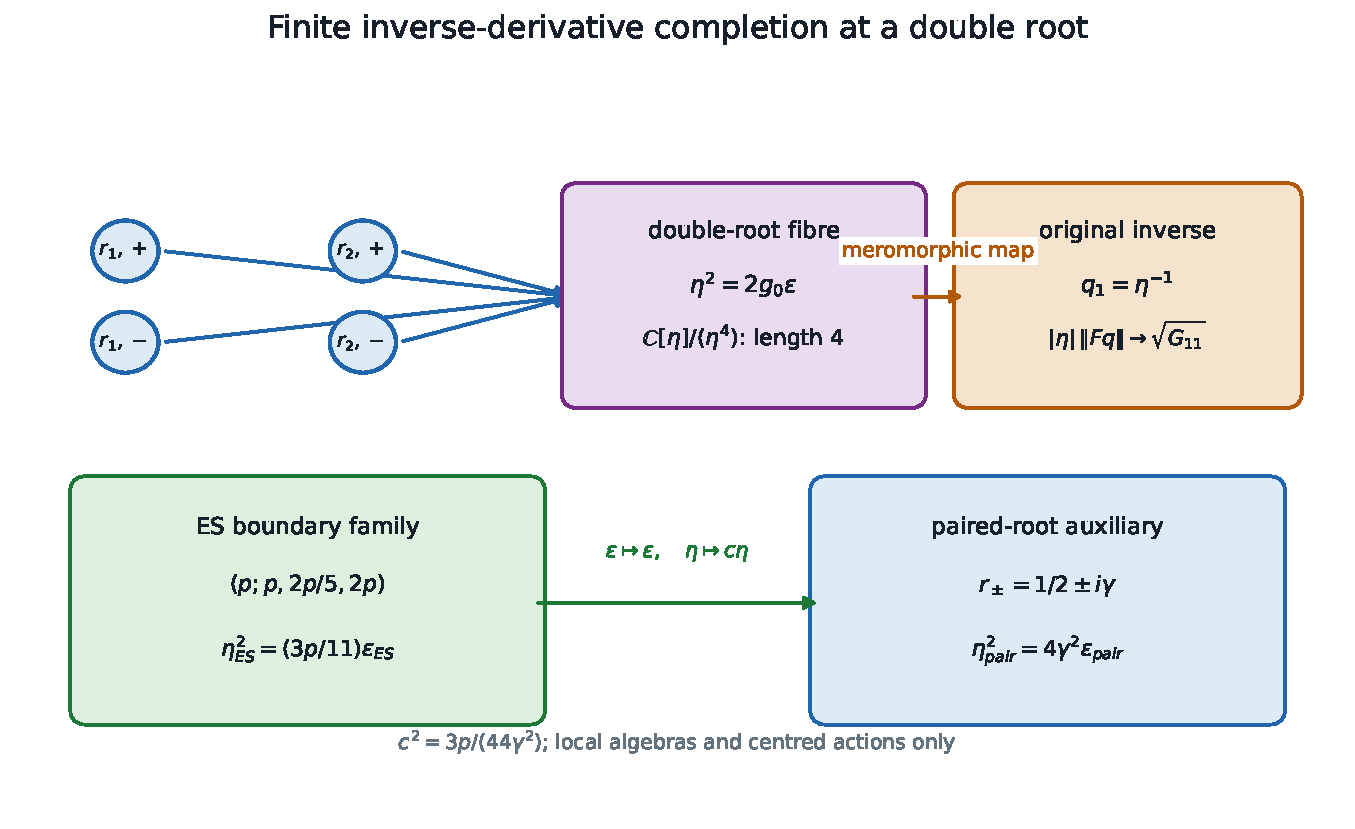
\includegraphics[width=.92\textwidth]{figures/finite-boundary-local-fibre.pdf}
\caption{The finite completion and its exact double-root fibre.  On
\(\eta\ne0\), \(\xi=\eta^{-1}\) recovers the original inverse.  At a double
root, four nearby signed states coalesce into the length-four algebra
\(\mathbb C[\eta]/(\eta^4)\), while the original first source coordinate keeps
its \(\eta^{-1}\) pole.  The lower arrow is the typed local algebra map EZ76;
it does not identify the global ES and paired-root constructions.  Reproduce
with \texttt{tools/generate\_20260920\_illustrations.py}.}
\label{fig:finite-boundary-local-fibre}
\end{figure}

\section{An invertible marked odd-moment frame}
\label{sec:odd-moment-frame}

On the ordered signed-root cover of the squarefree \(A\ne0\) coefficient
domain, retain the labels \(r_1,\ldots,r_4\) and signs
\(\xi_j^2h_u'(r_j)=1\), and define

\begin{equation}
 U=
 \begin{pmatrix}
 1&1&1&1\\
 r_1&r_2&r_3&r_4\\
 r_1^2&r_2^2&r_3^2&r_4^2\\
 r_1^3&r_2^3&r_3^3&r_4^3
 \end{pmatrix}
 \operatorname{diag}(\xi_1,\xi_2,\xi_3,\xi_4).        \tag{EZ77}
\end{equation}

\begin{theorem}[Odd-frame factorization and complete inverse]
\label{thm:odd-moment-frame}
One has

\begin{equation}
 \boxed{\det U=\frac{\chi}{A^2},\qquad\chi\in\{1,-1\}.}         \tag{EZ78}
\end{equation}

For each of the four component polynomials

\[
 1,\quad -\ii h_u',\quad A(h_u')^2+2rh_u',\quad
 \ii\bigl(7r^2h_u'-13(h_u')^2\bigr),
\]

reduce modulo \(h_u\), and let the corresponding ascending coefficient rows
in the ordered basis \(1,r,r^2,r^3\) be the rows of \(V_h\).  If \(O\) is the
original odd evaluation matrix EZ37, then

\begin{equation}
 \boxed{O=V_hU.}                                      \tag{EZ79}
\end{equation}

For \(m=U\beta\), the inverse is

\begin{equation}
\boxed{
\begin{aligned}
 \beta_j=\xi_j\bigl[&
 (C+Br_j+r_j^2+Ar_j^3)m_0\\
 &+(B+r_j+Ar_j^2)m_1
 +(1+Ar_j)m_2+Am_3\bigr].
\end{aligned}}                                      \tag{EZ80}
\end{equation}
\end{theorem}

\begin{proof}
The first matrix in EZ77 is the labelled Vandermonde matrix.  If
\(\Delta=\prod_{j<k}(r_k-r_j)\), then

\[
 \prod_jh_u'(r_j)=A^4\Delta^2,
 \qquad \left(\Delta\prod_j\xi_j\right)^2=A^{-4},
\]

which proves EZ78.  Evaluating the four reduced component polynomials at the
four roots and multiplying each column by its retained \(\xi_j\) gives EZ79.

For the inverse, synthetic division gives

\[
 \frac{h_u(r)}{r-r_j}=
 Ar^3+(1+Ar_j)r^2+(B+r_j+Ar_j^2)r
 +(C+Br_j+r_j^2+Ar_j^3).
\]

The corresponding Lagrange polynomial is this quotient divided by
\(h_u'(r_j)\).  Since
\(1/(\xi_jh_u'(r_j))=\xi_j\), applying the Lagrange coefficient functional
to \(m_0,m_1,m_2,m_3\) gives EZ80.
\end{proof}

Although \(U\) itself lives on the marked signed cover, EZ78--79 show that
the additional unmarked zero divisor of the original odd evaluation is
exactly \(\det V_h=0\), away from \(A\Disc(h_u)=0\).  At that divisor, moments
cannot be reconstructed from the already-collapsed data \(O\beta\); they must
be retained before applying \(V_h\).


\clearpage
\section*{The original integral signed completion}

The next proof works in the literal root basis \((p,x,y,z)\) over
\(\mathbb Z_p\).  It retains the original arithmetic lattice rather than
replacing a finite flat rank-eight algebra by an abstract vector space.

\begin{figure}[htbp]
\centering
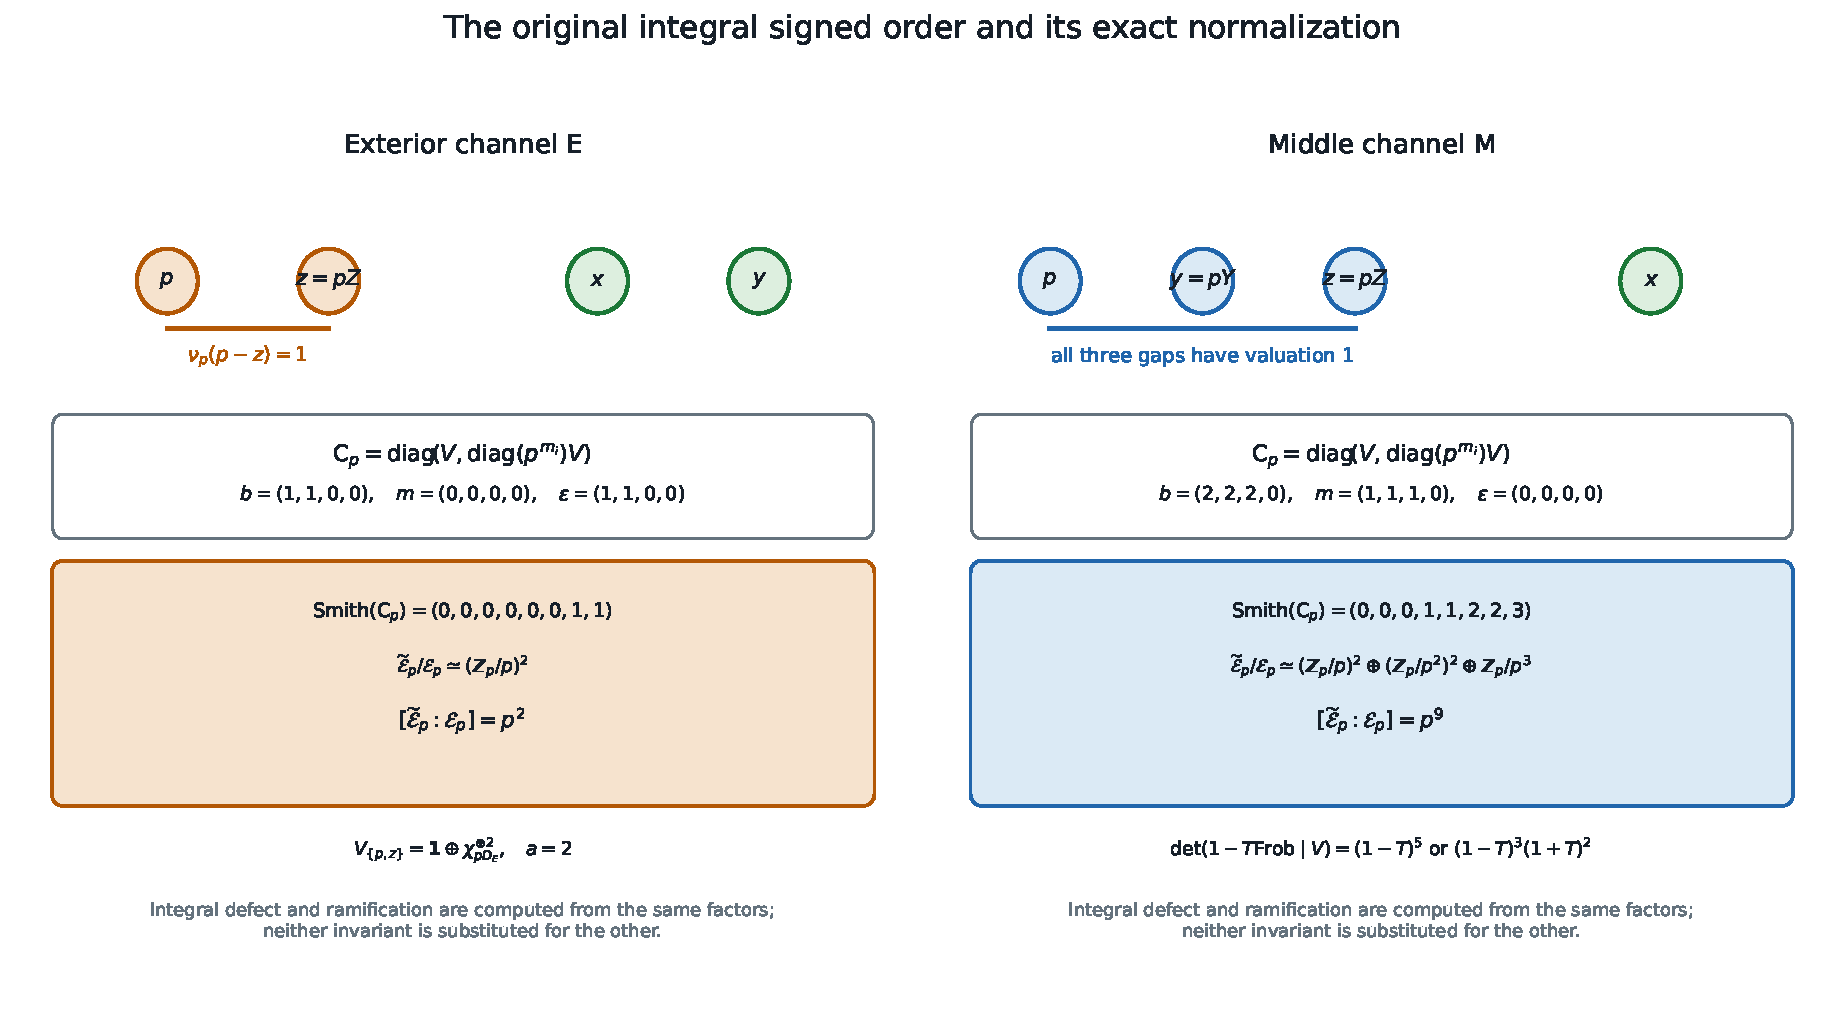
\includegraphics[width=\textwidth]{figures/integral-normalization-smith.pdf}
\caption{The exact normalization matrix and all Smith factors in the exterior
and middle channels.  The matrix, inverse lattice, quotient modules and
specialization kernels are proved in the following sections.}
\end{figure}

\section{Question, inherited objects, and the unresolved implication}
The preceding capacity theorem \cite{Capacity} completes a fixed-target divisor
problem. It proves that searching additional divisors at a fixed grade cannot
repair every exterior source. Its universal existence obligation is still open:
for a prescribed hard prime, produce an original exterior or middle state.
We do not assume that obligation in the present calculation.

The newly supplied ES--Zeta work \cite[\S\S1--3, equations (8)--(24)]{Input}
uses the \emph{literal} four roots $(p,x,y,z)$ and completes its signed inverse
by $\eta=\xi^{-1}$. Its monic equations give a finite flat rank-eight algebra.
The task here is to determine what happens to that particular algebra over
$\Z_p$, with its original coordinate lattice, rather than replacing it by an
arbitrary rank-eight vector space. The literal quartic is different from the
reciprocal cubic in \cite{Reciprocal}; the exact inversion and its derivative
twist are given in Section~\ref{sec:reciprocal}.

The Type-I/II identities are classical \cite[\S2, Propositions 2.2 and 2.6]{ET}.
Quadratic character restrictions are also antecedents; in particular compare
\cite[Corollary 1.3 and Appendix A]{BL}. All calculations needed for the local
and integral results below are proved explicitly. No historical-priority claim
is made for these specializations or for the standard local algebra tools.

\section{Original coordinates and the literal polynomial}
Fix a prime $p\equiv1\pmod{12}$. Thus $p\ge13$, and both $-1$ and $3$ are
squares modulo $p$. Set $K=\Q_p$, $\oo=\Z_p$, and normalize $\vp(p)=1$.
An original state retains
\[
 p/4<a<p/2,\quad R=4a-p,\quad u\mid a^2,
 \qquad E:R\mid4u+1,\qquad M:R\mid u+a.
 \tag{IC1}
\]
For $a=\prod_l l^{e_l}$ its original exponent vector is
$\beta_l=v_l(u)-e_l\in[-e_l,e_l]$. Let
\[
 g=\gcd(a,u),\qquad (h,r,s)=(g^2/u,u/g,a/g).
\]
Then $a=hrs$, $u=hr^2$, and $\gcd(r,s)=1$. The exact ordered returns are
\[
\begin{array}{ll}
 E:&\kappa=(pr+s)/R,\quad (x,y,z)=(a,hs\kappa,phr\kappa),\\
 M:&\lambda=(r+s)/R,\quad (x,y,z)=(a,phs\lambda,phr\lambda).
\end{array}                                                     \tag{IC2}
\]
Multiplication proves $4/p=1/x+1/y+1/z$. The ordered divisor inverses are
$a^2/(Ry-pa)$ and $pa^2/(Ry-pa)$, respectively. The middle complement
$u\mapsto a^2/u$ exchanges the last two denominators and is kept as an orientation,
not suppressed as a duplicate.

\begin{lemma}[Original character and unit facts]\label{lem:original}
Every factor in (IC2) is a $p$-unit. For each $d\mid a^2$,
$\Leg dR=\Leg dp$, with Jacobi symbol on the left. Consequently
\[
 E:\Leg hp=-1,\qquad M:\Leg{rs}p=-1.                      \tag{IC3}
\]
In the exterior case, $\kappa-r$ and $\kappa+r$ are $p$-units.
\end{lemma}
\begin{proof}
For an odd $l\mid a$, reciprocity and $R\equiv-p\pmod l$ give
$\Leg lR=\Leg{-1}l\Leg Rl=\Leg pl=\Leg lp$. If $2\mid a$, use
$R\equiv-p\pmod8$ and the supplementary law. Multiplication over the original
exponents proves the divisor identity. The E target is $-1/4$ modulo
$R\equiv3\pmod4$, so $\Leg up=-1$ and $u=hr^2$ gives the first assertion.
The M relation $r\equiv-s\pmod R$ gives the second.

The factors $h,r,s$ are below $p$. In E put
$\mathsf D=(4u+1)/R=(r+\kappa)/s$; the original identities give
$p\mathsf D+1=4hr\kappa$, so $\kappa$ is a unit too.
If $p\mid\kappa-r$, this identity gives $4hr^2\equiv1\pmod p$, contradicting
$\Leg hp=-1$. If $p\mid\kappa+r$, then $p\mid\mathsf D$ and
$4u+1=R\mathsf D$ gives the equally impossible nonresidue $u\equiv-1/4$.
For M, $r+s\le rs+1\le a+1<p$, so $\lambda<p$.
\end{proof}

The fixed, ordered root vector and scale are
\[
 (\ell_0,\ell_1,\ell_2,\ell_3)=(p,x,y,z),\qquad S=p+x+y+z,
\]
\[
 \mathcal H(T)=-S^{-1}\prod_{i=0}^3(T-\ell_i)
 =AT^4+T^3+BT^2+CT+D.                                   \tag{IC4}
\]
Here $D$ is a quartic coefficient, not the original exterior cofactor $\mathsf D$.
Vieta and the reciprocal identity give
\[
 A=-S^{-1},\quad C=5xyz/S,\quad D=-pxyz/S,
 \quad D=-pC/5,\quad B=-Ap^2-p-4C/(5p).                 \tag{IC5}
\]
These are the literal coefficient equations in \cite[\S2.1]{Input}; the prime
and every root label are retained. Define $d_i=\mathcal H'(\ell_i)$.

\begin{theorem}[Original prime-local root clusters]\label{thm:clusters}
The roots are distinct, $S\in\oo^\times$, and the following assertions hold.
For E write $(x,y,z)=(a,b,pc)$. Then $a,b,a-b,a+b$ are units,
$c\equiv1/4\pmod p$, and
\[
 (\vp(d_0),\vp(d_1),\vp(d_2),\vp(d_3))=(1,0,0,1),
 \qquad \vp\Disc(\mathcal H)=2.                         \tag{IC6}
\]
For M write $(x,y,z)=(a,pb,pc)$. Then $b,c,b-c,b-1,c-1$ are units,
\[
 4bc\equiv b+c\pmod p,\qquad\Leg{bc}p=-1,
\]
\[
 (\vp(d_0),\vp(d_1),\vp(d_2),\vp(d_3))=(2,0,2,2),
 \qquad \vp\Disc(\mathcal H)=6.                         \tag{IC7}
\]
In coefficient order $(A,B,C,D)$ the valuations are respectively
$(0,0,1,2)$ and $(0,1,2,3)$.
\end{theorem}
\begin{proof}
For E, $c=hr\kappa$ and $4c=p\mathsf D+1$. The remaining unit statements follow
from Lemma~\ref{lem:original} and $a\pm b=hs(r\pm\kappa)$.
Thus exactly one pair of roots, $p$ and $pc$, has difference of valuation one;
all other differences are units. In particular they are all distinct, and
$S\equiv a+b$ is a unit. The derivative and discriminant formulas prove (IC6).
The coefficient $B\equiv-ab/S$ is a unit, and (IC5) gives the other valuations.

For M, $b=hs\lambda,c=hr\lambda$. The unit and distinctness of $b,c$ follow from
$r\ne s$, $r,s<p$; equality would force $r=s=1$ and $R\mid2$.
The ES equation gives $4bc=pbc/a+b+c$, and (IC3) gives $\Leg{bc}p=-1$.
If $b=1\pmod p$, then $c=1/3$, making $bc$ a square since $\Leg3p=1$.
The same excludes $c=1$. The three roots $p,pb,pc$ therefore have pairwise
valuation-one differences; the singleton $a$ is separated by units. Now
$S\equiv a$, giving (IC7). In $B$ the leading term is
$-pa(1+b+c)/S$, and $1+b+c\equiv1+4bc$ cannot vanish, since $bc=-1/4$
would be a square. Hence $\vp(B)=1$. The remaining values follow from (IC5).
\end{proof}

In particular any two original E and M coefficient targets at the same prime
have distance exactly one in the maximum $p$-adic norm on $(A,B,C,D)$: the
$B$-coordinate is a unit on E and divisible by $p$ on M, while all coordinates
are integral. An infinitesimal target deformation preserving reduction is not
such a channel change. No comparison with a complex Gamma metric is inferred.

\section{The rank-eight generic algebra and its original integral order}
The supplied completion specializes, with its exact original basis, to
\[
 \OO=\oo[T]/(\mathcal H),\qquad
 \SSS=\OO[\eta]/(\eta^2-\mathcal H'(T)).                 \tag{IC8}
\]
The leading coefficient $A$ is a unit, so both equations can be made monic.
Thus $\SSS$ is free over $\oo$ on
\[
 1,T,T^2,T^3,\eta,\eta T,\eta T^2,\eta T^3.             \tag{IC9}
\]
After inverting $\eta$ it is the original signed inverse, with
$\xi=\eta^{-1}$ and $\xi^2\mathcal H'(T)=1$.
The full physical Fabel coordinates, inherited from \cite[equation (21)]{Input}, are
\[
 \left(\eta^{-1},-T-i\eta,
 A\eta^3+2T\eta+3i\eta^2,
 7iT^2\eta+(B-17T+AT^2)\eta^2-13i\eta^3-2A\eta^4\right).       \tag{IC10}
\]
Either embedding of $i$ in $K$ may be chosen and is kept fixed. No complex
period coefficient is presumed to have a $p$-adic descent.

Over $K$, root evaluation gives exactly
\[
 \SSS_K\simeq\prod_{i=0}^3K[\eta_i]/(\eta_i^2-d_i).     \tag{IC11}
\]
There is no infinity factor: $A\ne0$ and all four roots are finite.
This is not the seven-dimensional reciprocal-cubic algebra.

\begin{theorem}[Generic local signed types]\label{thm:fields}
An E state has either
\[
 K^4\times K_{\rm ram}^2
 \quad\text{or}\quad K_{\rm unr}^2\times K_{\rm ram}^2,
                                                                  \tag{IC12}
\]
and consequently four or zero $K$-rational signed inverse points.
An M state has either
\[
 K^8\quad\text{or}\quad K^4\times K_{\rm unr}^2,          \tag{IC13}
\]
and consequently eight or four such points. Repeated field factors retain their
root labels; they are not identified.
\end{theorem}
\begin{proof}
For E the two valuation-one derivatives have square ratio: after dividing by
$p$ their ratio is $-1\pmod p$. They define the same ramified quadratic extension.
At the other two roots the derivative residues are
\[
 -\frac{a^2(a-b)}{a+b},\qquad -\frac{b^2(b-a)}{a+b}.
\]
Their ratio is a square, so either both split or both define the unramified
quadratic extension. This proves (IC12).

For M, divide the three cluster derivatives by $p^2$. Their unit residues are
\[
 (1-b)(1-c),\quad(b-1)(b-c),\quad(c-1)(c-b).              \tag{IC14}
\]
Their product is the negative of a nonzero square. Since $-1$ is a square,
either all three or exactly one are squares. At the singleton,
$d_1\equiv-a^2$ is a square. This proves (IC13).

For the local facts, a square unit modulo the odd prime has unique compatible
lifts after a sign is chosen: if $z_n^2\equiv d\pmod{p^n}$, set
$z_{n+1}=z_n+p^nk$, with
$k\equiv-(z_n^2-d)/p^n\,(2z_n)^{-1}\pmod p$.
A nonsquare unit has irreducible separable quadratic reduction and gives the
unramified quadratic extension. An odd-valuation class gives a ramified
quadratic. These are also the standard constructions in
\cite[Chapter 7, Newton's lemma and local extensions]{Milne}.
\end{proof}

At the single hard prime $p=1009$, all four alternatives occur. The respective
original $(a,u)$ and ordered denominators are
\[
\begin{array}{c|c|c}
\text{channel, number of }K\text{-points}&(a,u)&(x,y,z)\\\hline
E,0&(253,11)&(253,87032,3818056)\\
E,4&(253,23)&(253,86020,7890380)\\
M,8&(253,11)&(253,2042216,88792)\\
M,4&(253,23)&(253,1021108,92828).
\end{array}                                                   \tag{IC15}
\]
These are four independently checked original states. In particular a
$K$-rational point on the literal signed fibre is not a necessary condition for
an ES witness. Every row still has eight geometric characteristic-zero points.

\section{Exact normalization, conductors and invariant factors}
Put $k_i=\lfloor\vp(d_i)/2\rfloor$ and
\[
 \theta_i=\eta_i/p^{k_i},\qquad
 \delta_i=d_i/p^{2k_i},\qquad
 N_i=\oo[\theta_i]/(\theta_i^2-\delta_i),\qquad
 \NN=\prod_iN_i.                                         \tag{IC16}
\]
Each $\delta_i$ is a unit or has valuation one. Thus $N_i$ is the maximal
integral order in its generic factor. For a field factor, integrality of
$a+b\theta_i$ first gives $a\in\oo$ by its trace. Its norm then gives
$2\vp(b)+\vp(\delta_i)\ge0$, forcing $b\in\oo$ because $\vp(b)$ is integral.
For a split unit factor use the two values $a\pm b\sqrt{\delta_i}$ and the
unit $2\sqrt{\delta_i}$. This also proves maximality without an unspecified
integral basis.

The precise normalization map is
\[
 f(T)+\eta g(T)\longmapsto
 \bigl(f(\ell_i)+p^{k_i}g(\ell_i)\theta_i\bigr)_{i=0}^3,
 \qquad \deg f,\deg g<4.                                \tag{IC17}
\]
It is injective: over $K$, evaluate at all distinct labelled roots.
All its inverse coefficients are provided by the corresponding Lagrange
polynomials, so its integral image can be tested without changing the lattice.

\begin{theorem}[Complete original integral defect]\label{thm:index}
For E,
\[
 \NN/\SSS\simeq(\oo/p)^2,
 \qquad[\NN:\SSS]=p^2,
 \qquad\mathfrak f_E=pN_0\times N_1\times N_2\times pN_3.       \tag{IC18}
\]
For M,
\[
 \NN/\SSS\simeq(\oo/p)^2\oplus(\oo/p^2)^2\oplus\oo/p^3,
 \qquad[\NN:\SSS]=p^9,
\]
\[
 \mathfrak f_M=p^3N_0\times N_1\times p^3N_2\times p^3N_3.      \tag{IC19}
\]
Here $\mathfrak f=\{n\in\NN:n\NN\subseteq\SSS\}$ is the conductor ideal in
this finite algebra. It is not the analytic weighted conductor of the Zeta
programme. In the eight-dimensional original basis, the Smith exponents are
\[
 E:(0,0,0,0,0,0,1,1),\qquad
 M:(0,0,0,1,1,2,2,3).                                   \tag{IC20}
\]
\end{theorem}
\begin{proof}
Unit differences split off every noncolliding root integrally, by the polynomial
CRT. For E, the remaining root lattice on the pair $p,pc$ is exactly
\[
 L_2=\{(z_0,z_3)\in\oo^2:z_0-z_3\in p\oo\}.
\]
A linear interpolation proves sufficiency, since $p-pc$ is $p$ times a unit.
Both coefficients $f$ and $g$ in (IC17) give a copy of $L_2$: here $k_i=0$.
This proves the quotient and exponents. A normal element supported at just one
of these two roots is in the original order precisely when its coefficients
of $1$ and $\theta_i$ both lie in $p\oo$. The resulting $pN_i$ is an ideal and
is maximal with this property, giving (IC18).

For M, order the cluster as $p,pb,pc$ and use the Newton polynomial basis
$1,T-p,(T-p)(T-pb)$. Evaluation gives diagonal factors $1,p,p^2$ times units,
and integral row operations remove the lower entries. Thus its root lattice
$L_3$ has quotient $\oo/p\oplus\oo/p^2$. The two coefficients in (IC17)
give $L_3\oplus pL_3$. Their exponents are $(0,1,2)$ and $(1,2,3)$; the
singleton contributes two zeros. This proves (IC19)--(IC20).

For the conductor, a vector supported at one of the three roots has a unique
Lagrange interpolation of degree at most two. Its leading coefficient has
denominator of exact order $p^2$. Hence a normal value $a+b\theta_i$ supported
there belongs to $\SSS$ precisely when $a\in p^2\oo$ and $b\in p^3\oo$.
For it to lie in the conductor, multiplication by the unit $\theta_i$ must also
belong to the order. This forces $a,b\in p^3\oo$, and that condition is
sufficient because $1,\theta_i$ is the full normal basis. The singleton is
already maximal. This proves the displayed conductor.
\end{proof}

The root orders alone have indices $p$ (E) and $p^3$ (M), with Smith exponents
$(0,0,0,1)$ and $(0,0,1,2)$. A further exact check is the trace discriminant:
\[
 \vp\Disc(\SSS)=2\vp\Disc(\OO)+\sum_i\vp(4d_i)
 =6\ (E),\quad18\ (M).
\]
The normal algebra has discriminant valuation two (E) or zero (M). The square
of the change-of-basis determinant again gives index exponents two and nine.
Neither determinant is a density or positivity assertion.

\begin{corollary}[The original actions on the finite defect module]
Let $Q=N/\widehat S$, a module rather than a quotient ring. Multiplication by the
original $T$ and $\eta$ descends to it. Their exact nilpotence indices are
\[
 E:(1,2),\qquad M:(3,3),                                \tag{IC20a}
\]
respectively. Thus the finite quotient retains nonzero action, even though
rational extension removes it.
\end{corollary}
\begin{proof}
The quotient is supported only at the colliding roots. For E, $T$ is divisible
by $p$ there and $\eta^2=d_i$ is also divisible by $p$, so the conductor kills
both actions. Multiplying a supported normal constant by $\eta$ still has a
coefficient not divisible by $p$ and is nonzero in $Q$.
For M, both $T^3$ and $\eta^3$ have a factor $p^3$ at each colliding normal
factor. But their squares, applied to a supported normal $\theta_i$, have a
$\theta_i$-coefficient of exact valuation two. The membership criterion in the
proof of Theorem~\ref{thm:index} requires three, so both squared actions remain
nonzero. All the normal root quotients are units, precluding cancellation.
\end{proof}

\paragraph{Complete inverse coordinates.}
For a normal vector $a_i+b_i\theta_i$, interpolate the four values $a_i$ to
obtain $f(T)$, and the values $b_i/p^{k_i}$ to obtain $g(T)$. Membership in the
original order means all eight coefficients of $f,g$ are in $\oo$. Thus (IC17)
has an explicit partial integral inverse and a total $K$-linear inverse.
The quotient in (IC18) or (IC19) is retained when the integral inverse fails.
There is no $\oo$-linear splitting of its surjection from $\NN$, since that
would map a nonzero torsion module into a torsion-free one.

\section{Boundary fibres and a sharp finite lifting obstruction}
At E, the colliding factor of the special fibre is
\[
 \F_p[\epsilon,\eta]/(\epsilon^2,\eta^2-2g_0\epsilon)
 \simeq\F_p[\eta]/(\eta^4),\qquad g_0=-ab/S\ne0.         \tag{IC21}
\]
At M it is
\[
 \boxed{\F_p[\epsilon,\eta]/(\epsilon^3,\eta^2-3\epsilon^2).} \tag{IC22}
\]
These follow from the actual reduced quartics, respectively
$-S^{-1}T^2(T-a)(T-b)$ and $T^3(1-T/a)$, using the supplied
multiple-root algebra \cite[equation (23)]{Input}. Their dimensions are four
and six. Multiplication by $\epsilon$ has blocks $(2,2)$ or $(3,3)$.
Multiplication by $\eta$ has blocks $(4)$ or $(4,2)$: on
$1,\epsilon,\epsilon^2,\eta,\epsilon\eta,\epsilon^2\eta$ in (IC22), its
successive ranks are $6,4,2,1,0$. Thus (IC22) is not a single length-six chain.

The normalization map modulo $p$ has kernel dimension two on the E collision
block and five on the M collision block. For E, $T$ becomes zero in each normal
factor modulo $p$, while $\eta$ gives its two labelled nonzero nilpotents. For M,
both $T=p\zeta$ and $\eta=p\theta$ become zero in the normal special fibre.
These are the kernels dictated by (IC20), not a deletion of the original labels.

\begin{theorem}[The added E point stops at the third digit]\label{thm:lift}
The point $(T,\eta)=(0,0)$ of (IC21) has exactly $p$ lifts solving both original
equations modulo $p^2$, and has no lift modulo $p^3$.
\end{theorem}
\begin{proof}
Write $\mathcal H(T)=U(T)(T-p)(T-pc)$, with
$U(T)=-(T-a)(T-b)/S$ a unit near zero. A putative lift modulo $p^2$ is
$T=pw,\eta=pv$, with $w,v\in\F_p$. The first equation is automatic. The
second gives
\[
 0\equiv pU(0)(2w-1-c)\pmod{p^2},
\]
so $w=(1+c)/2=5/8\pmod p$. The $p$ values of $v$ are all possible.
For any higher lift of that $T$,
\[
 \frac{\mathcal H(T)}{p^2}\equiv
 -U(0)\frac{(1-c)^2}{4}
 =\frac{9ab}{64S}\not\equiv0\pmod p.                   \tag{IC23}
\]
Thus the root equation already fails modulo $p^3$, independently of $\eta$.
\end{proof}

The finite flat completion is proper, but this boundary point has no integral
$\oo$-section. The ramified generic points remain over their actual quadratic
extensions. At $p=1009$ in the first row of (IC15), the entire generic signed
fibre has no $K$-point despite an original ES solution and a rational special
boundary point. No smooth Hensel hypothesis is available at $\eta=0$.

For M, the collision block instead has the exact integral normalization chart
\[
 G(Z)=(Z-1)(Z-b)(Z-c),\qquad
 G(Z)=0,\quad \theta^2=\frac{a-pZ}{S}G'(Z),              \tag{IC24}
\]
with $T=pZ,\eta=p\theta$. This is finite etale of rank six, since the reduced
roots are distinct and the right side is a unit there. The inverse divides
exactly by those powers of $p$. The character product in (IC14) proves that
at least one cluster root has two $K$-rational signed lifts. Thus the M boundary
point does lift to $\oo$, although its full multiplicity and the index $p^9$
are still retained.

The original physical inverse (IC10) has pole $\vp(\xi)=-1/2$ on the E cluster
and $\vp(\xi)=-1$ on the M cluster. Inverting $\eta$ in (IC21) or (IC22)
annihilates that local algebra; it does not turn the added state into a finite
original affine inverse. The supplied complex metric limit remains the one in
\cite[equations (21)--(22)]{Input}; no identification of that complex norm with
this nonarchimedean valuation is asserted.

\section{The generic prime-sign symmetry has an integral defect}
The distinguished-root projector is
\[
 e_p(T)=\frac{\prod_{i=1}^3(T-\ell_i)}{\prod_{i=1}^3(p-\ell_i)}.
                                                               \tag{IC25}
\]
Its values are $(1,0,0,0)$. Its coefficients require an exact denominator $p$
in E and $p^2$ in M, since its numerator is monic and the denominator has
those respective valuations. This is also the supplied $g_p/d_p$ projector
\cite[equations (9)--(11)]{Input}.

Among the supplied four generic deck sign maps, the prime-only flip is
\[
 T\longmapsto T,\qquad \eta\longmapsto(1-2e_p(T))\eta.
                                                               \tag{IC26}
\]
Uniqueness in the original free basis (IC9) proves that it does not preserve
$\SSS$. Nor does its negative, the denominator-only flip. The identity and the
simultaneous sign $\eta\mapsto-\eta$ do preserve it. All four extend to the
normalization (IC16), where their action is an independent sign on the labelled
quadratic factors. This conclusion concerns those four source deck maps, not
all automorphisms of a specialized split algebra.

\section{Literal channel interpolation and reciprocal inversion}
Suppose actual E and M states are both supplied at the same $p$. Denote their
ordered literal roots by $x_i$ and $y_i$. The exact root-algebra maps are
\[
 F(T)=\sum_i y_i\frac{\prod_{j\ne i}(T-x_j)}{\prod_{j\ne i}(x_i-x_j)},
 \qquad
 G(T)=\sum_i x_i\frac{\prod_{j\ne i}(T-y_j)}{\prod_{j\ne i}(y_i-y_j)}.
                                                               \tag{IC27}
\]
Evaluation proves both inverse compositions on the respective quotient rings.
Under their common label coordinates in $K^4$, the integral orders obey
\[
 \OO_M\subset\OO_E,
 \qquad[\OO_E:\OO_M]=p^2.                              \tag{IC28}
\]
Indeed the three M cluster values are congruent modulo $p$, in particular at
the E pair of labels $0,3$. The already proved indices give the ratio.
Thus $F$ is integral. In the reverse interpolation, the summand at label $2$
has unit output $x_2$ and a denominator of valuation two; the other cluster
outputs are divisible by $p$. Consequently
\[
 \boxed{\min_j\vp(G_j)=-2,\qquad
 p^2G(T)\bmod p=c_0T^2(T-a_M),\quad c_0\ne0.}           \tag{IC29}
\]
This proves the exact lost factor, not just an upper denominator estimate.
At $p=1009$, the pair of $(a,u)=(253,11)$ states in (IC15) gives
$c_0=306$ and $p^2G\equiv275T^2+306T^3\pmod{1009}$.

The full signed generic algebras need not be isomorphic over $K$: E has ramified
field factors and M has none. The surviving comparison is explicit after a
specified extension. Adjoin square roots $\delta_i^2=d_i^M/d_i^E$ and send
$\eta_M$ to $\delta(T)\eta_E$, where $\delta$ is the labelled interpolation
of the $\delta_i$. The inverse uses their reciprocals. The extension has degree
at most four: for odd $p$, unit classes are square or a fixed nonsquare unit,
and the only additional parity is that of $p$. The original integral images
must still be tested by (IC17); they are not made unit lattices by this field
isomorphism.

This is applicable to actual source-changing returns, for example the preceding
capacity certificate \cite[sharp finite repair]{Capacity} at $p=825241$:
\[
 E:(a,R,u,h,r,s,\kappa)=(206321,43,2240439739,19,10859,1,208402140),
\]
\[
 M:(a,R,u,h,r,s,\lambda)=(217170,43439,25,1,5,43434,1).
\]
The latter is supplied there by the noncanonical original cofactor word $25$,
not by interpolation in (IC27). The current certificate transports both actual
states through (IC18)--(IC29), preserving their different factor inventories.
No M state is assumed to exist in order to use (IC27) as an existence proof.

\subsection{The reciprocal model changes the lattice and the signed square class}
\label{sec:reciprocal}
Keep all four roots while applying $z_i=p/\ell_i$. On the literal root algebra,
\[
 \boxed{I(T)=-\frac pD(AT^3+T^2+BT+C)=p/T.}              \tag{IC30}
\]
Its exact coefficient denominator is $p$ in E and $p^2$ in M. The transformed
monic polynomial is $Z^4L(p/Z)/L(0)$, where $L=\prod(T-\ell_i)$.
If $N=\prod_i\ell_i$ and the normalized reciprocal quartic is
$\widetilde{\mathcal H}=-\frac15\prod(Z-z_i)$, differentiation gives
\[
 \boxed{\widetilde{\mathcal H}'(z_i)=
 \omega\frac{\mathcal H'(\ell_i)}{\ell_i^2},\qquad
 \omega=-\frac{p^3S}{5N}.}                              \tag{IC31}
\]
The four reciprocal roots sum to five; the coefficient $-1/5$ is therefore
fixed, not fitted. The signed comparison needs the recorded quadratic twist
$\sqrt\omega$. Its valuation is one in E and zero in M.

The reciprocal discriminant valuation is the literal value plus
$12-6\vp(N)$, hence two in E and zero in M. The reciprocal root order has
index $p$ in E and is maximal in M. In E its colliding labels are now $1,2$,
not $0,3$. Removing the separately marked root $z_0=1$ yields the preceding
reciprocal cubic, whose signed derivatives acquire the further factors
$-(z_i-1)/5$ from the augmented quartic. This states the maps and square classes
rather than conflating the earlier seven-point and current eight-point fibres.

\section{A single missing prime passes any fixed finite integrality window}
The supplied real separation estimates \cite[\S1.2, equations (2)--(4)]{Input}
are necessary at an integral witness. The next result gives a precise scope
test for treating them, together with a finite local completion, as sufficient.
It retains both numerical channel gates and the entire allowed numerical range
of the proposed integer $u$. The one failed condition is original square-divisor
availability, at one explicitly designated prime.

\begin{theorem}[A joint, single-prime source obstruction]\label{thm:controls}
For every fixed finite set of rational primes $\Sigma$, there are infinitely
many hard primes $p$ and integers $a,R,u$ such that
\[
 p/4<a<p/2,\quad R=4a-p=3,\quad0<u<a^2,
 \quad R\mid4u+1,\quad R\mid u+a,                       \tag{IC32}
\]
yet $u\nmid a^2$. There is just one extra prime occurrence in $u$, at a
specified prime $l\notin\Sigma\cup\{p\}$. In particular
\[
 a^2/u\in\Z_q\quad(q\in\Sigma\cup\{p\}),
 \qquad v_l(a^2/u)=-1.
\]
The literal E and M rational denominator returns from these same numerical
coordinates satisfy the ES identity and all the following conditions:
\begin{enumerate}
\item their only nonintegral denominator has reduced denominator exactly $l$;
\item at $p$ they have the respective E and M local signatures, normalization
indices, conductors and invariant factors proved above;
\item their four positive literal roots have successive gaps greater than one;
\item with $s_p=(p^2+3p)/4$ and $B_p=p+s_p(s_p+1)$, both satisfy
\[
 S<B_p,\quad\max(x,y,z)<s_p(s_p+1)/3,\quad
 \Disc(\mathcal H)\ge144/B_p^6,\quad
 2/S\le|\mathcal H'(\ell_i)|\le S^2;
\]
\item the same prime $p$ has separately supplied original integer E \emph{and}
M states. The failed source in (IC32) is not an ES counterexample.
\end{enumerate}
\end{theorem}
\begin{proof}
Choose a prime $l\equiv11\pmod{12}$ outside $\Sigma$. Dirichlet's theorem
\cite[Theorem 18.1]{Dirichlet} permits this choice, and then supplies infinitely
many primes in the reduced CRT progression
\[
 p\equiv1\pmod{840},\qquad p\equiv-1\pmod l.
\]
The moduli are coprime. Take $p>4l$ and set
\[
 a=(p+3)/4,\quad R=3,\quad u=al,\quad
 h=a/l,\quad r=l,\quad s=1,\quad
 \kappa=(pl+1)/3,\quad\lambda=(l+1)/3.                  \tag{IC33}
\]
Both quotients are positive integers, and $l<a$ gives $0<u<a^2$.
Modulo three, $p\equiv a\equiv1$ and $l\equiv2$, so both gates hold.
But $a\equiv1/2\pmod l$ and $\gcd(a,u)=a$. Thus $h=a/l$ is nonintegral with
exact denominator $l$. Every prime of $a$ occurs in $u$ with its original
exponent; the only extra coordinate is $v_l(u)=1$, while $v_l(a)=0$.
In the centered original box this is exactly $\beta_l=1$ outside $[0,0]$.
All the equations $a=hrs$, $u=hr^2$, and $\gcd(r,s)=1$ hold, but the positive
rational grade $h$ is not an allowed original integer grade.

The two explicit returns are
\[
 E_{\rm rat}:\quad(a,a\kappa/l,pa\kappa),\qquad
 M_{\rm rat}:\quad(a,pa\lambda/l,pa\lambda).              \tag{IC34}
\]
Multiplication proves their reciprocal identities. Since $p,a,\kappa,\lambda$
are all units at $l$, the middle displayed denominator has exact reduced
denominator $l$ and the other two are integers. Every declared finite place
therefore passes the denominator test and the original divisor valuation test.

At the original prime, $p\nmid a,l,\kappa,\lambda$ and
$(l/p)=(p/l)=(-1/l)=-1$. Also $a\equiv3/4\pmod p$ is a square. Thus the same
unit and character calculations as Theorem~\ref{thm:clusters} apply to (IC34):
in the first return $4a\kappa\equiv1$, while the second has normalized root
product $a^2\lambda^2/l$ a nonsquare. The reduction patterns, local field
alternatives and all integral normalization formulas follow exactly. This
verifies local algebra for rational targets; it does not insert a missing
integer factor into the original box.

For both triples write their largest denominator as $z=s_p q$,
where $q=\kappa$ or $\lambda$ and $s_p=pa$. Since $l<a$,
$\kappa=(pl+1)/3<(s_p+1)/3$, and the same bound holds for $\lambda$.
Hence $z<s_p(s_p+1)/3$. Their other denominator is $z/(pl)$ in E and $z/l$ in M.
It is greater than $pa/3>p+1$; also $p-a>1$ and $z-y>1$. Thus the ordered root
list $a,p,y,z$ has successive gaps greater than one, and
$S=p+a+y+z<p+3z<B_p$. Four such roots have Vandermonde modulus at least twelve.
The product of three differences at a selected root is at least two and at most
$S^3$. The claimed discriminant and derivative bounds follow from
$\mathcal H=-S^{-1}\prod(T-\ell_i)$.

Finally retain the genuine endpoint data
\[
 R_E=l,\quad a_E=u_E=(p+l)/4,\quad
 (h_E,r_E,s_E,\kappa_E)=(a_E,1,1,(p+1)/l).
\]
They are integral and return $(a_E,a_E\kappa_E,pa_E\kappa_E)$.
There is also a genuine middle state: put
$j=(l+1)/4$, $c=(p+1)/l$, then
\[
 (h_M,r_M,s_M,\lambda_M)=(j,1,c,1),\quad a_M=jc,\quad
 R_M=c+1,\quad u_M=j.
\]
Its identity is $p=lc-1=4jc-c-1$. Since $l\ge11$ and $c>4$, both first-half
inequalities hold. This gives the last assertion without assuming ES.
\end{proof}

For $\Sigma=\{2,3,5,7,11\}$, choose $l=23$ and the hard prime $p=35281$.
The numerical source is
\[
 a=8821,\quad R=3,\quad u=202883,
 \quad(h,r,s,\lambda,\kappa)=(8821/23,23,1,8,270488).
\]
The two nonintegral denominator triples are
\[
 \boxed{E_{\rm rat}=(8821,2385974648/23,84179571556088),}
\]
\[
 \boxed{M_{\rm rat}=(8821,2489709608/23,2489709608).}      \tag{IC35}
\]
The E target has zero rational local signed points and the M target has four.
Their local normalization and ramification types are different. The only forbidden original factor is
$23\mid u$, while $23\nmid a=8821$. A second complete example at $p=54601$ is
included in the certificate. Trial division proves these displayed primes.

This theorem does not concern all places simultaneously: the omitted place is
explicit. Nor does it exclude an adaptive test of every possible denominator
prime. It proves that a fixed finite collection of local observations, even
with the original numerical ranges, both channel congruences and the stated
real bounds, is not original square-divisor membership. For the broader
arithmetic-approximation context, compare \cite[Theorems 1.1, 1.8--1.9]{BL}.
The separate companion fragment \texttt{crt\_control\_note.tex} preserves an
additional exact CRT construction with three larger-prime control targets;
those targets and their full equations are also independently checked.

\section{Verification scope, information loss, and continuation}
The full replay covers every original first-half box for the 99 primes
$p\equiv1\pmod{12}$ through 3000: 868359 square divisors and 4505 labelled
states, of which 2451 are E and 2054 are oriented M. It compares all derivative
valuations, characters, coefficient identities and local point alternatives.
The deep lattice calculations expand every original normalization matrix at
the four $p=1009$ examples. The separate checker uses all minors for the
invariant factors and independent Lagrange inversion, rather than the first
program's elimination. Both test the direct $p^2/p^3$ boundary equations, the
actual capacity crossing, and every supplied rational control.

The main verifier is standard-library Python. The separate implementation imports
none of it or of the preceding work. Its original source enumeration is by
primitive coprime $r,s$ and $h=a/(rs)$, rather than by divisors of $a^2$.
The prime domains, original vectors, ordered states and finite computation
ranges are all recorded in JSON. Checks of a finite prefix are not a proof
that the original source is nonempty at every prime.

No source coefficient is created by normalization. The exact sequence
$0\to\SSS\to\NN\to\NN/\SSS\to0$ retains all the finite torsion coordinates
in (IC18)--(IC20). Taking a quotient, a rational extension, or a reduction modulo
$p$ is accompanied by its calculated kernel. A receiving zero is not relabelled
as absence of an original divisor word, and an added nilpotent boundary point
is not promoted to an original E/M word. The countermodels in
Theorem~\ref{thm:controls} make that latter distinction quantitative.

The remaining Turn~7 task is still to force a positive original integer
coefficient for each prescribed hard prime. The completed same-grade capacity
classification remains available, and its actual source-changing maps are
compatible with the lattice comparison here. Finite rank, properness, local
normalization and the displayed approximation bounds do not supply the initial
arithmetic state by themselves. No Turn~8 witness guarantee, universal ES
proof, Lean build or independent mathematical review is claimed.


\clearpage
\section*{Defining-prime normalization, gluing and local characters}

The general collision calculation below includes the separated exterior and
middle orders as exact specializations and then keeps every additional
closer-pair valuation.  Its translated chart is related to the original chart
by a quadratic twist whose square class is retained.

\begin{figure}[htbp]
\centering
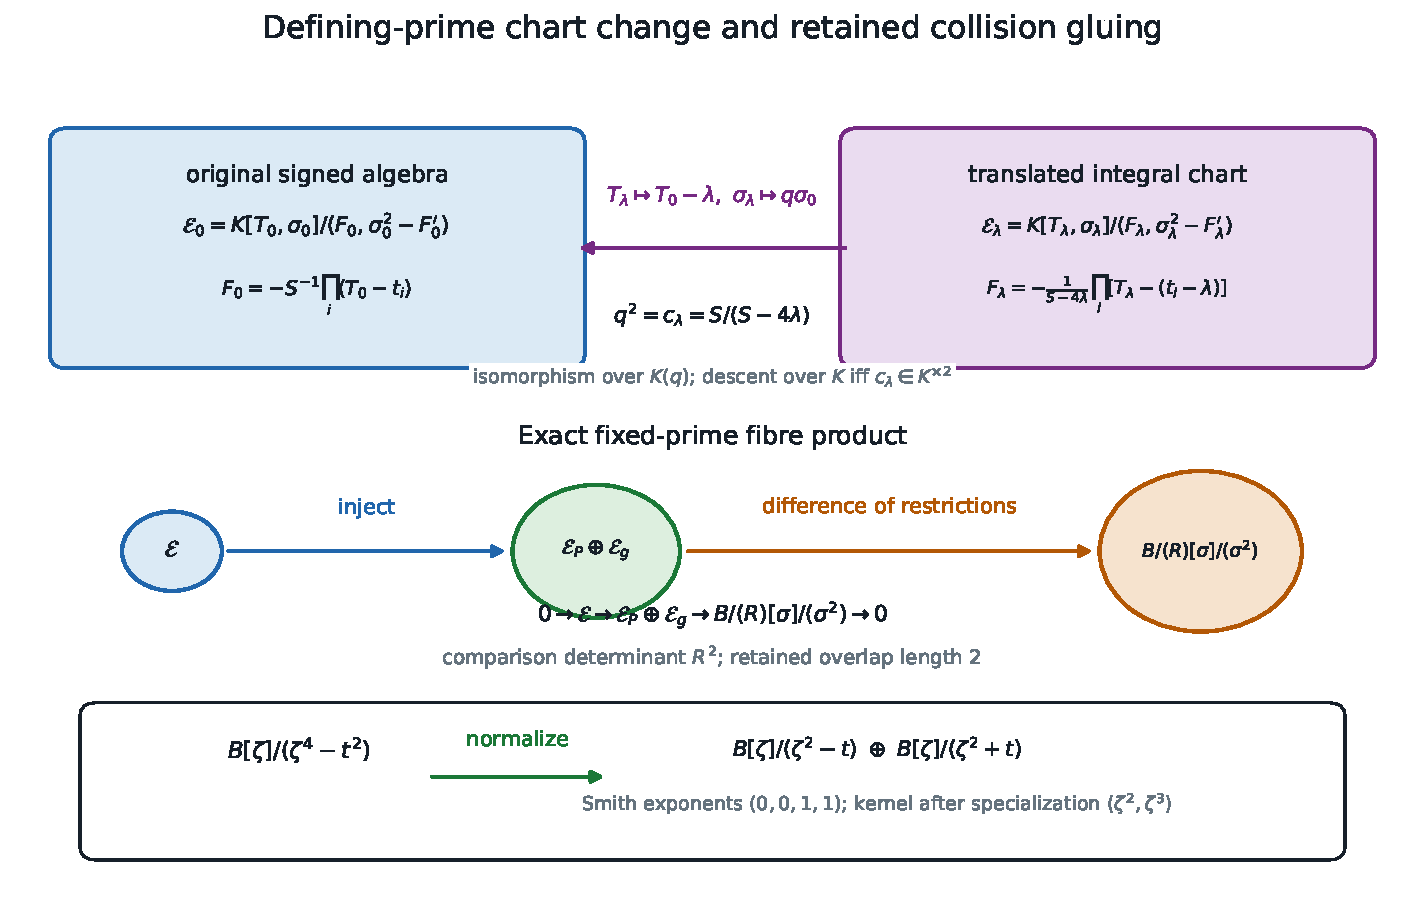
\includegraphics[width=\textwidth]{figures/defining-prime-twist-gluing.pdf}
\caption{The exact translated-chart quadratic twist, rank-\(2+6\) fibre
product and collision normalization.  The displayed base extension is part
of the map and is not discarded during descent.}
\end{figure}

\input{DEFINING_PRIME_CONTINUATION}

\clearpage
\input{INTEGRAL_NORMALIZATION_CROSSWALK}

\clearpage
\input{LOCAL_GALOIS_REPRESENTATION}

\section{A root-algebra bridge and its exact projective obstruction}

After choosing a bijection \(t_j\leftrightarrow\rho_{*,j}\) between the four
distinct ES roots and the four fixed reference roots, let
\(\ell_j^\rho(S)\) be the Lagrange polynomial satisfying
\(\ell_j^\rho(\rho_{*,k})=\delta_{jk}\).  Then
\begin{equation}
 \Theta:\frac{\C[T]}{\prod_j(T-t_j)}\longrightarrow
 \frac{\C[S]}{\prod_j(S-\rho_{*,j})},\qquad
 [f]\longmapsto\sum_{j=1}^4 f(t_j)[\ell_j^\rho(S)]     \tag{EZ36}
\end{equation}
is a unital algebra isomorphism.  Its inverse evaluates at the reference roots
and interpolates at the ES roots; hence both kernels are zero.  It depends on
the chosen bijection.  It is generally not induced by one fractional-linear
map.  Such a map exists exactly when the corresponding ordered cross ratios
agree, up to the six values produced by relabelling.  This is the exact
projective obstruction; failure of that stronger map does not erase EZ31--36.

\section{Scope of the quartic-to-conductor core}

The new composite is
\[
\begin{array}{c}
\text{actual ordered ES exterior state}\\
\downarrow\ \text{EZ18--23}\\
(p;x,y,z)\\
\downarrow\ \text{normalized product EZ6}\\
J_4\in\mathcal B,\quad p=-5u_4/u_3,\quad G(J_4)=0\\
\downarrow\ P^{-1}\\
\{q_{p,\pm},q_{x,\pm},q_{y,\pm},q_{z,\pm}\}\\
\downarrow\ (\Phi_*,\Psi_*,T_{A,*})\\
\text{eight states in the fixed weighted-conductor square.}
\end{array}
\]
The map begins with an actual ES witness and therefore is not a proof that a
witness exists for every \(p\).  The hypersurface \(G=0\) is not by itself an
arithmetic occupancy theorem.  The fixed quartet and fixed conductor data do
not vary with \(p,x,y,z\), and the construction proves no zero of the Riemann
zeta function.  The signed-root monodromy group of order \(192\) belongs to the
generic eight-sheet cover over \(\mathcal B\).  After restricting to a fixed
intrinsic prime and to \(\mathcal B_p\),
Theorem~\ref{thm:fixed-input-monodromy} gives the different order-\(48\) group
and its rank-\(2+6\) sheet decomposition.  Neither group is
attributed to the seven-state boundary suspension.  The finite completion
EZ67 adds nonreduced collision fibres but leaves the original meromorphic
inverse pole visible; its local paired-root map does not identify the global
ES and zeta constructions.

\clearpage
\section*{Illustrated guide to the new five-track continuation}

The following three figures display the proved maps without replacing their
coordinate formulas.  Tracks I--III refine the ES/Fable interfaces.  Tracks
IV--V are RH-facing conditioning and certification interfaces and are not
claims of progress toward ES occupancy.

\begin{figure}[htbp]
\centering
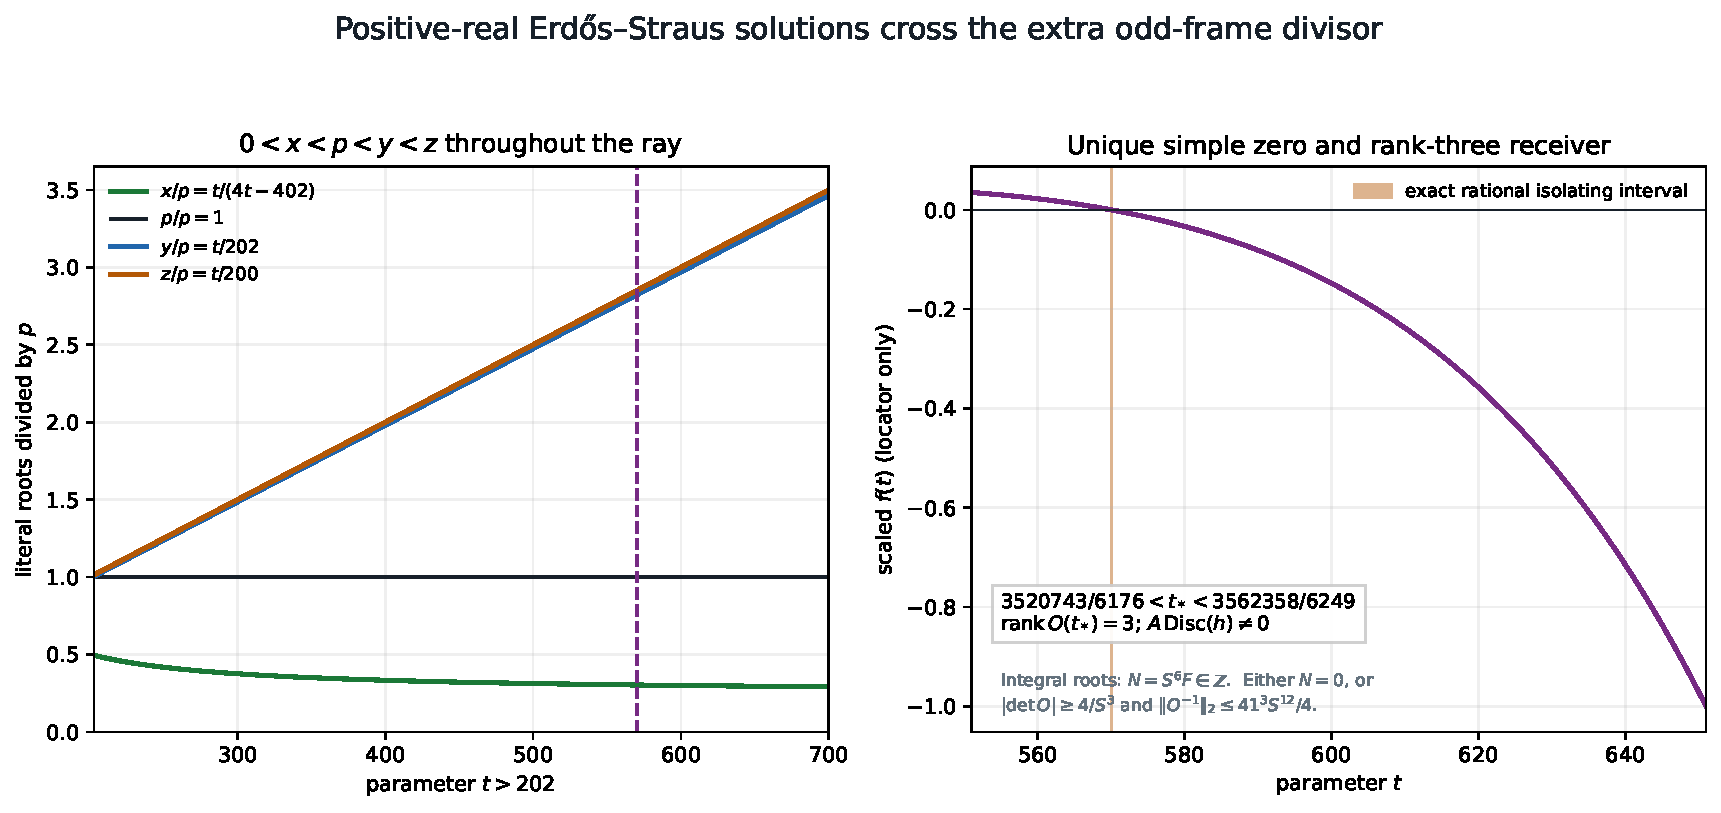
\includegraphics[width=\textwidth]{figures/positive-real-receiving-divisor.pdf}
\caption{The exact positive-real solution ray and its unique rank-three odd
receiver.  The plotted polynomial is a locator; the rational isolating
interval, Sturm count, nonzero minor and integral dichotomy are proved in
Track~I, Sections~3--4.}
\end{figure}

\begin{figure}[htbp]
\centering
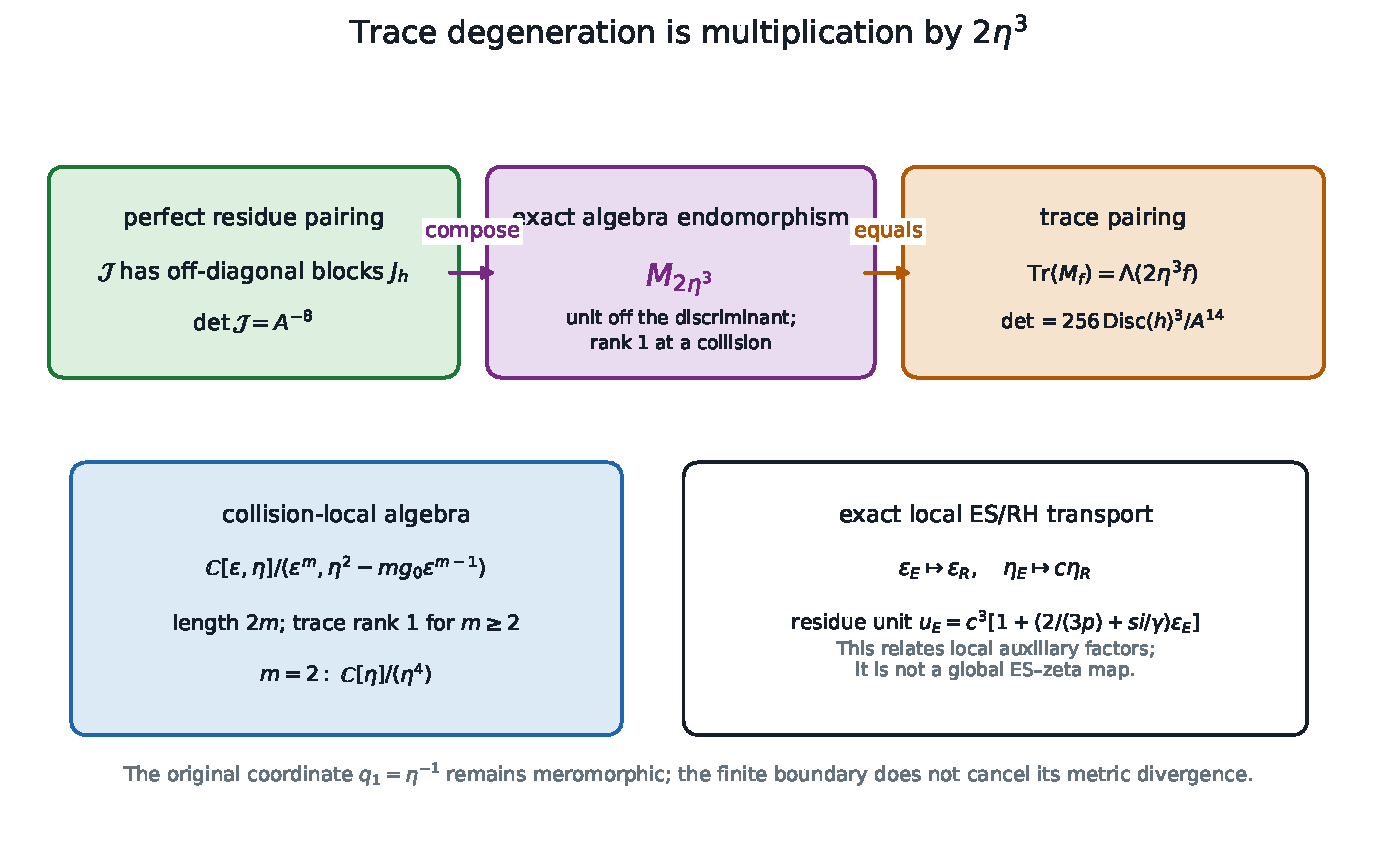
\includegraphics[width=\textwidth]{figures/residue-trace-factorization.pdf}
\caption{The perfect residue pairing reaches the trace pairing through the
specific endomorphism \(M_{2\eta^3}\).  Track~II, Sections~3--5 prove the
determinants, collision ranks, local algebra and nonconstant residue unit.}
\end{figure}

\begin{figure}[htbp]
\centering
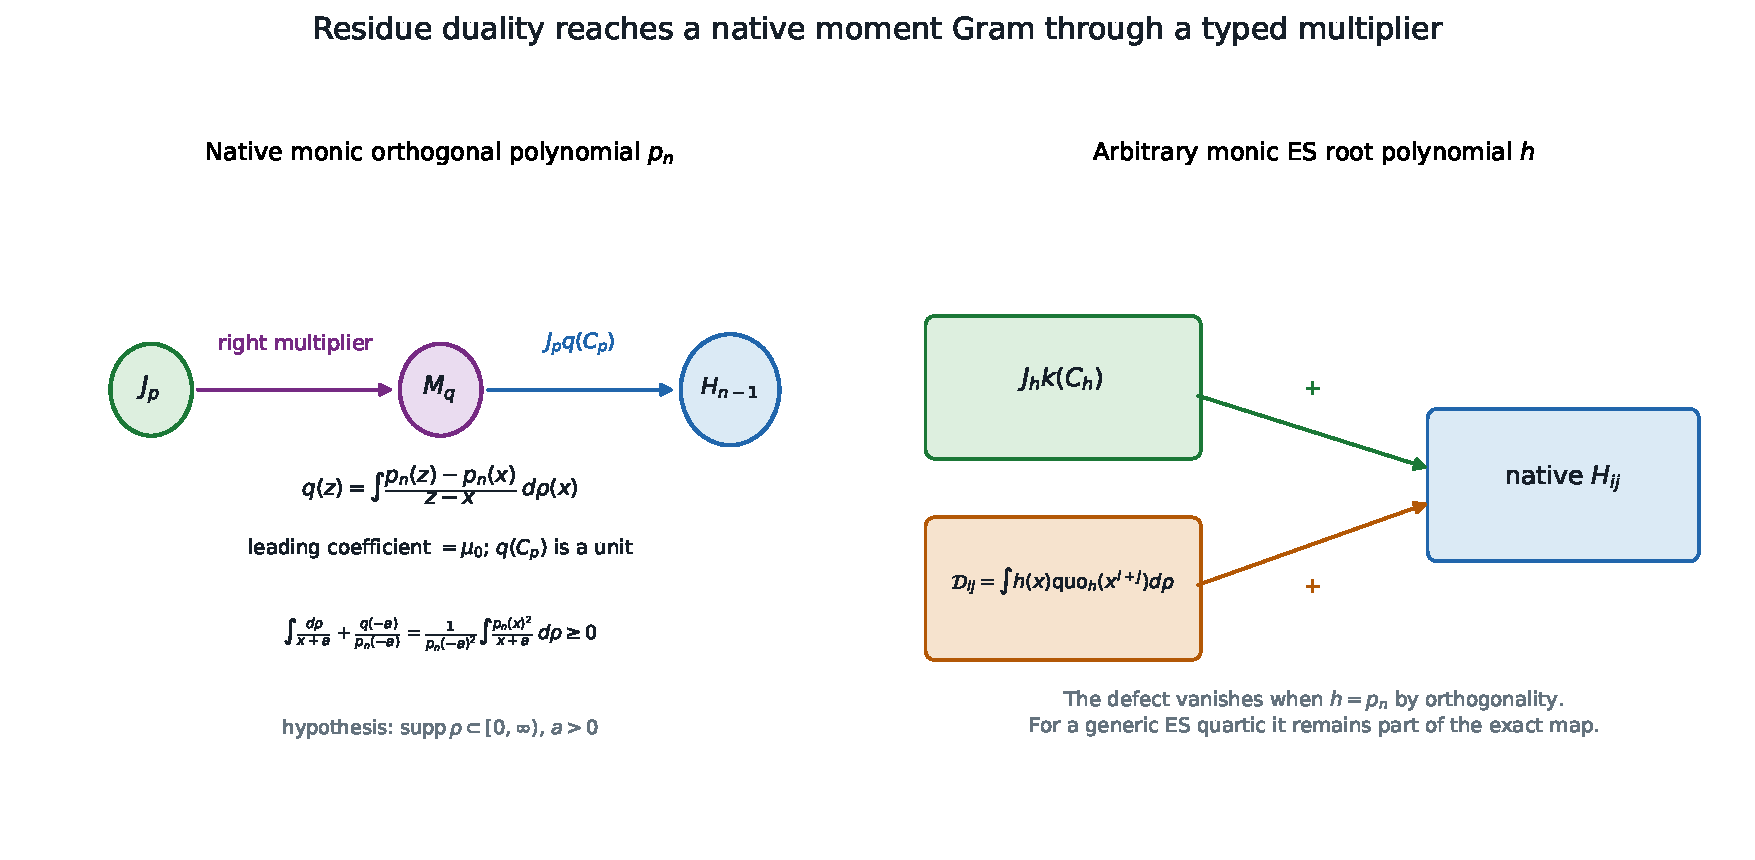
\includegraphics[width=\textwidth]{figures/residue-native-gram-bridge.pdf}
\caption{The native orthogonal-polynomial multiplier and the stronger
arbitrary-polynomial identity retaining its relation defect.  Track~III proves
the multiplier, support hypothesis, resolvent error and defect term.}
\end{figure}

\clearpage
\input{ES_RH_MULTI_CONTINUATION}

\clearpage
\section*{Arithmetic-frame and signed-descent continuation}

The final continuation keeps four proof tracks separate: arithmetic
nonsingularity of the ES receiving frame, a sharp paired native determinant
return, finite heat-action remainders in the retained metric, and an exact
finite-field signed-cover descent calculation.

\begin{figure}[htbp]
\centering
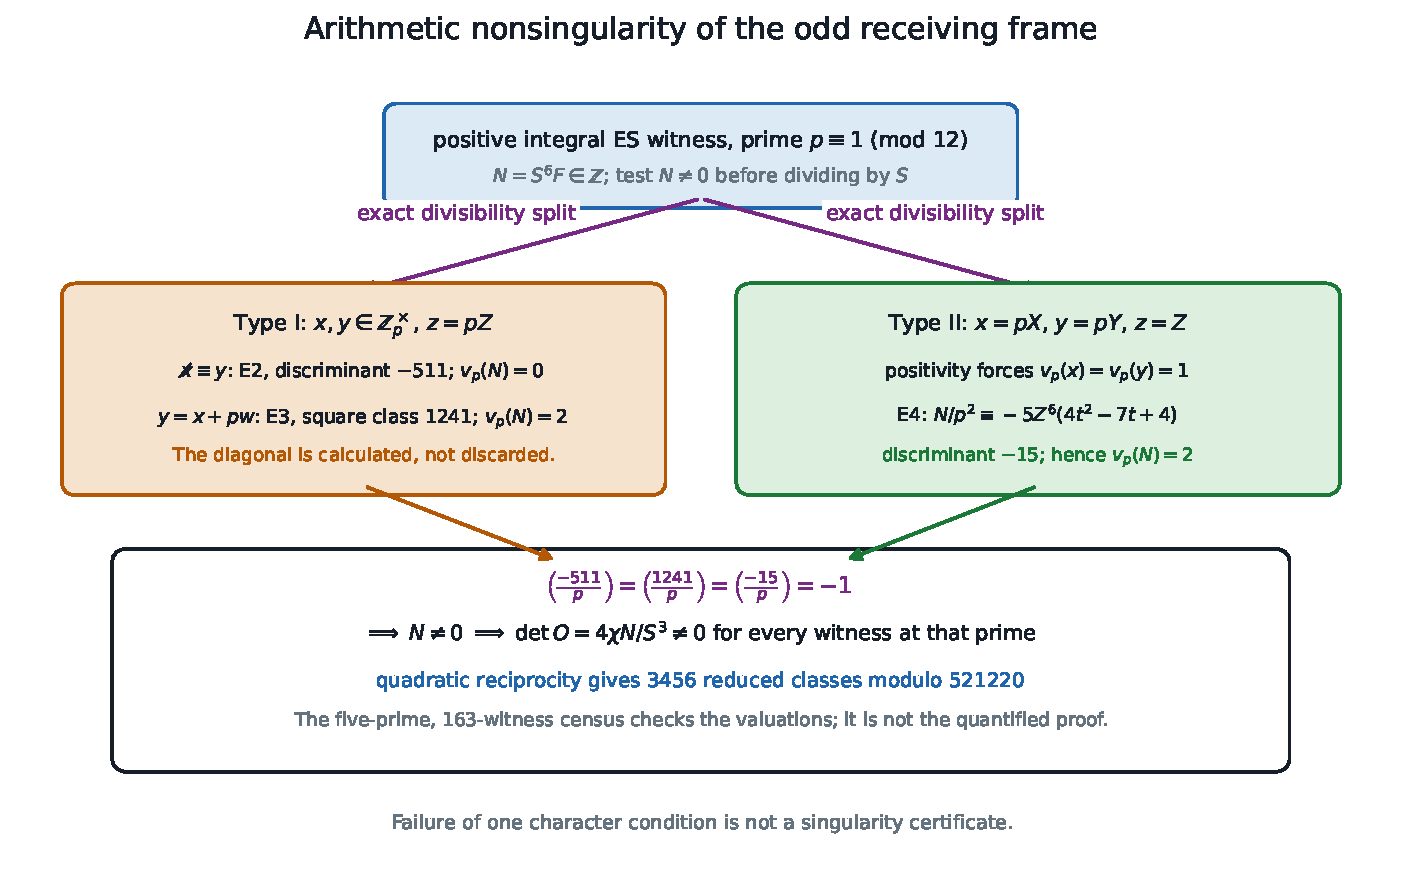
\includegraphics[width=\textwidth]{figures/arithmetic-frame-sieve.pdf}
\caption{The exhaustive valuation split and the three quadratic obstructions
used to force receiving-frame nonsingularity.}
\end{figure}
\clearpage

\begin{figure}[htbp]
\centering
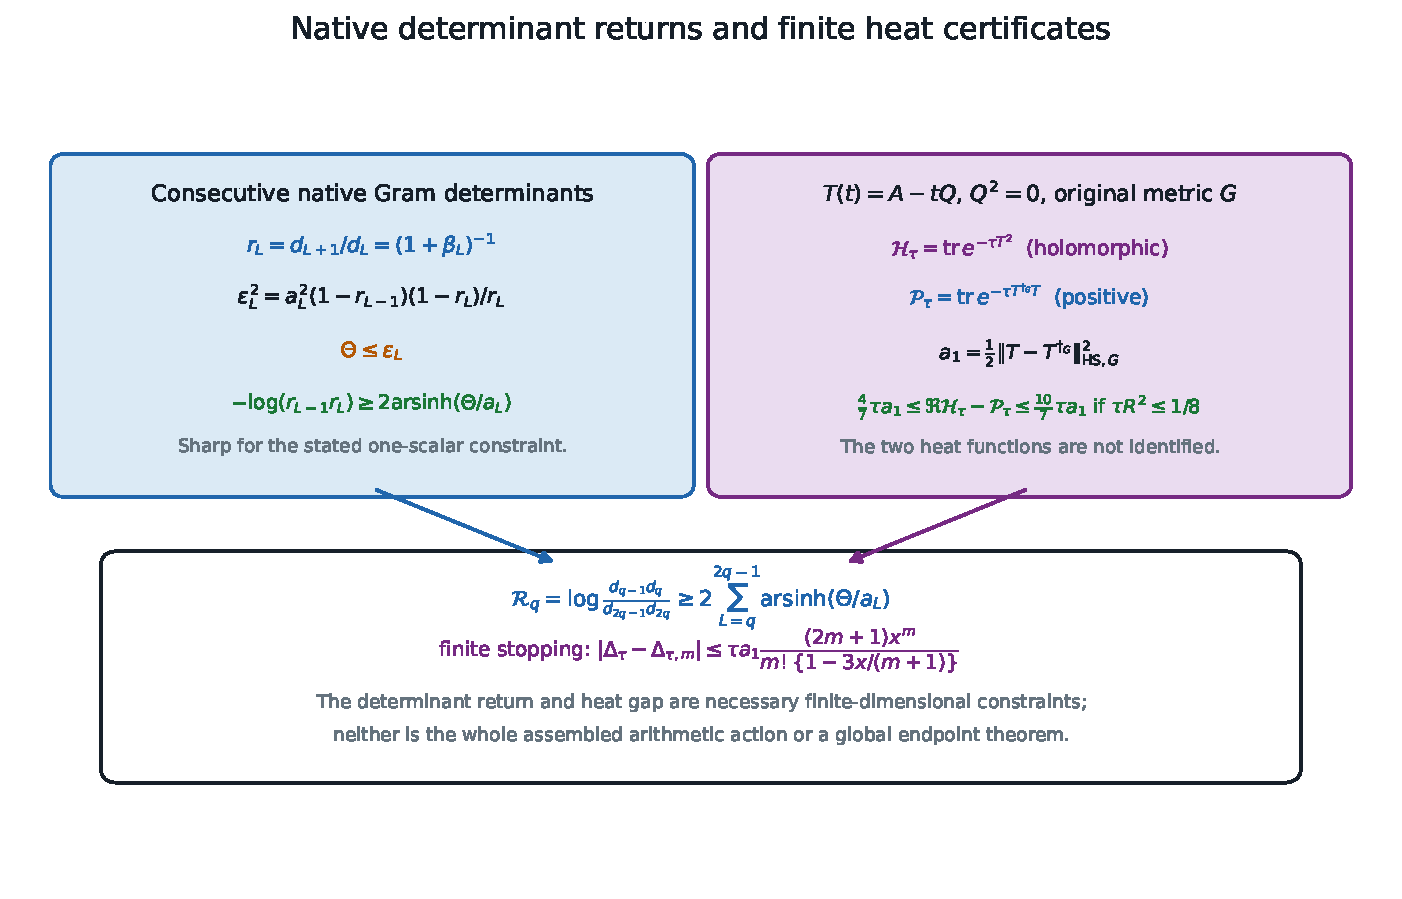
\includegraphics[width=\textwidth]{figures/determinant-heat-mechanism.pdf}
\caption{The exact determinant-ratio identity, its sharp two-ratio
consequence, and the two distinct heat actions with their proved remainder
boundary.}
\end{figure}
\clearpage

\begin{figure}[htbp]
\centering
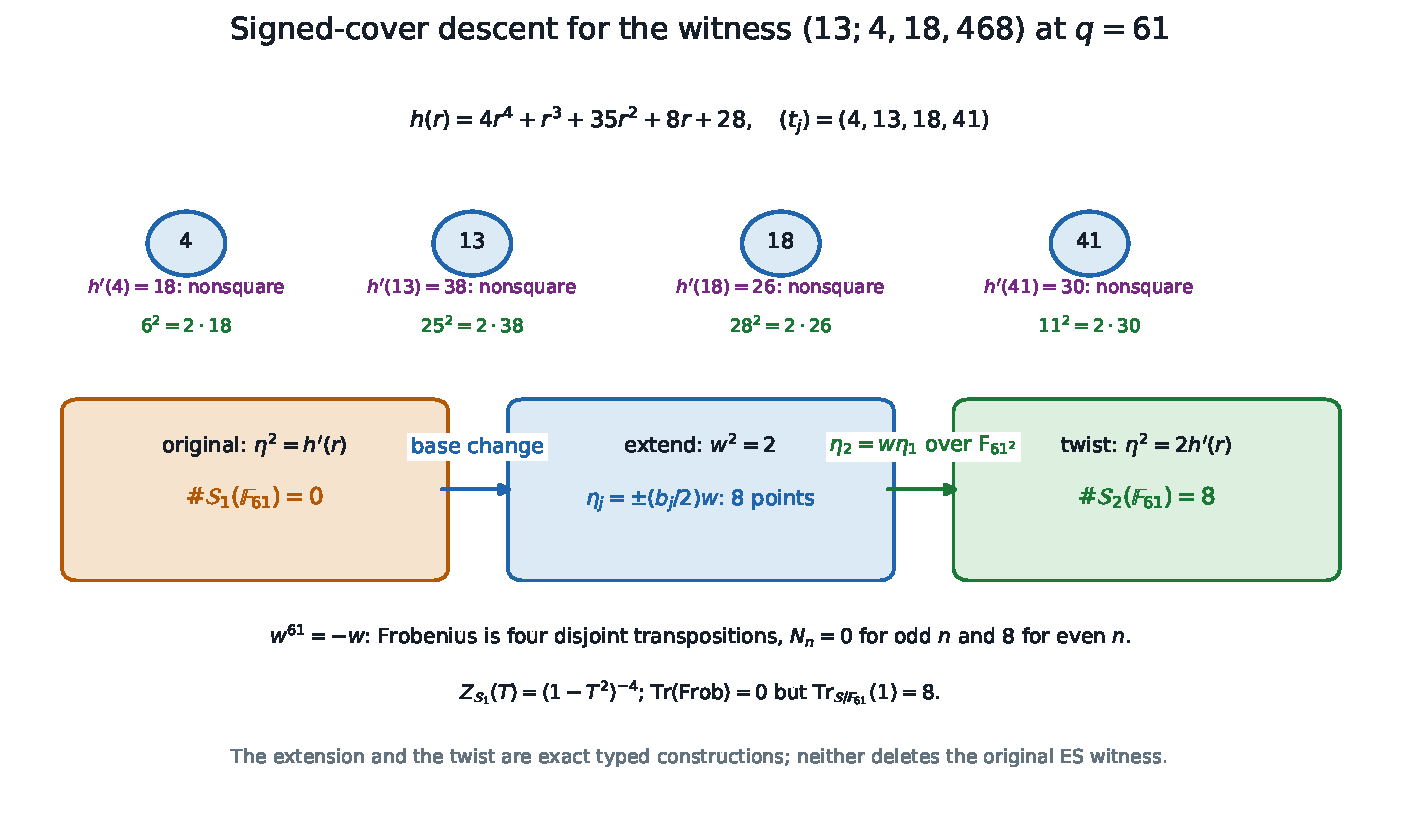
\includegraphics[width=\textwidth]{figures/finite-field-twist-descent.pdf}
\caption{The original signed cover and its nonsquare twist for
\((13;4,18,468)\) at \(q=61\), including the quadratic base-extension map and
Frobenius action.}
\end{figure}
\clearpage

\input{ES_RH_CONTINUATION_B}

\clearpage
\section{Cumulative scope and remaining arithmetic problem}

Every theorem in this reader starts either from an actual positive integral
Erd\H{o}s--Straus witness or from an explicitly stated algebraic, local or
finite-dimensional input.  The integral normalization and finite-field
descent theorems classify what happens after such a witness is present.  The
three-character theorem proves receiving-frame nonsingularity on its stated
residue classes conditional only on witness existence; failure of one of its
characters does not imply singularity.  The determinant and heat estimates
are exact finite-dimensional constraints in their retained metric and are not
substituted for the assembled arithmetic action.

The unresolved ES statement remains the original occupancy problem: for each
hard prime, force at least one positive integral exterior or middle source.
No finite signed fibre, normalization, nilpotent completion, conductor index,
local Galois character, Gram determinant, heat remainder or CRT control family
supplies that source by itself.  Likewise, none of the proved root-algebra,
weighted-conductor or finite-field maps identifies an ES root with a
nontrivial zero of the Riemann zeta function.

\begin{thebibliography}{99}
\small\raggedright

\bibitem{ET}
C. Elsholtz and T. Tao,
\emph{Counting the number of solutions to the Erd\H{o}s--Straus equation on
unit fractions},
J. Aust. Math. Soc. 94 (2013), 50--105,
\texttt{arXiv:1107.1010}, Section 2.
The Type-I/Type-II coordinates used in EZ28a--d are traced to Propositions
2.2 and 2.6.

\bibitem{Hatcher}
A. Hatcher,
\emph{Topology of Numbers},
American Mathematical Society, 2022, Section 6.4.
Used only for the stated quadratic-reciprocity and supplementary laws; their
specialization to the retained ES factors is proved in EZ28e.

\bibitem{Dirichlet}
A. V. Sutherland,
\emph{18.785 Number Theory I, Lecture 18},
Massachusetts Institute of Technology, 2017, Theorem 18.1.
Used for Dirichlet's theorem in the two reduced arithmetic progressions of
Theorems~\ref{thm:sharp} and \ref{thm:obstruct}; both progressions and their
coprimality conditions are constructed explicitly before the theorem is
applied.

\bibitem{BL}
M. Bright and D. Loughran,
\emph{Brauer--Manin obstruction for Erd\H{o}s--Straus surfaces},
Bull. London Math. Soc. 52 (2020), 746--761,
\texttt{arXiv:1908.02526}, Corollary 1.3, Theorems 1.1 and 1.8--1.9,
and Appendix A.
Used for the cited antecedent character restrictions and the arithmetic
surface context; every local specialization asserted here is proved in the
reader.

\bibitem{Milne}
J. S. Milne,
\emph{Algebraic Number Theory},
course notes, version 3.08, 2020, Chapter 7, pp. 119--130.
Used for Newton--Hensel lifting and the standard classification of unramified
and Eisenstein quadratic extensions; the required digit lift is displayed in
the proof of Theorem~\ref{thm:local-fibre}.

\bibitem{ESC123}
The Clankers,
\emph{Erd\H{o}s--Straus--Fable C123 preprint},
canonical local corpus unit \texttt{PUBUNIT-1C9A160031EECC8F3F032D4D},
source lines 22314--22543.
Used for the generic quartic product/resultant carrier, the ES incidence
\(\Res=1,4af-be=0\), and the constant-Jacobian chart.  The normalized
prime--denominator target, intrinsic-prime formula, image hypersurface and
global-locus refinement are proved here.

\bibitem{ESReader}
The Clankers,
\emph{Erd\H{o}s--Straus Project Reader},
Zenodo record 21845035, version 69, 2026,
\url{https://zenodo.org/records/21845035}.
The three-dimensional transport reproduced in
Theorem~\ref{thm:transported-raw-tetrahedron} is the theorem labelled
\texttt{thm:Fable-ES-raw-tetrahedron-quarter-altitude} in the archived
source; its exact checker is
\texttt{verification/verify\_fable\_es\_raw\_tetrahedron.py}.

\bibitem{Turn7}
The Clankers,
\emph{Small-shape rigidity and channel rescue},
\texttt{../es-turn07-shape-rigidity-20260919/core.tex},
20 September 2026.
Used for EZ18--23, including every exterior gate and the marked-cubic inverse.

\bibitem{Turn7Fabel}
The Clankers,
\emph{Prime-local Fabel fibres and same-prime negative-square channel
transfers},
\texttt{../es-turn07-fabel-arithmetic-bridge-20260920/corrected/workbench.tex},
20 September 2026.
The received 30-file packet and its hashes remain unchanged; the corrected
build supplies the exact alpha inverse-fibre gate, the derivative-residue
wording repair, and the full proofs used in EZ28a--z.

\bibitem{SignedCover}
The Clankers,
\emph{The ES--Fable inverse correspondence in the original weighted conductor},
\texttt{upstream/FABLE\_TO\_ORIGINAL\_CONDUCTOR.tex},
FC1--FC71, GF1--GF28, SE1--SE18 and SM1--SM19,
20 September 2026.
Used for the four-dimensional map, complete inverse, image complement,
nonproper locus, conductor square, signed evaluation and monodromy.  The frozen
cumulative source hash is
\texttt{bfb75ff468f35b71103ad2671e22f20fee0414df4a43d1dab5fc2d19aabbd1b6}.

\bibitem{Input}
The Clankers and the Split-Zero programme,
\emph{Combined continuation: literal ES quartic, fixed-input monodromy,
finite rank-eight completion and native error bounds},
preserved source \texttt{received/combined-continuation-20260920.txt},
20 September 2026.
Used at the exact equation locators cited in the integral-completion proof;
the preserved source and corrected public derivation remain separate.

\bibitem{Reciprocal}
The Clankers,
\emph{Prime-local Fable fibres and same-prime negative-square channel
transfers},
\texttt{../es-turn07-fabel-arithmetic-bridge-20260920/corrected/workbench.tex},
20 September 2026.
Used for the reciprocal cubic and its seven-point chart, which the present
reader relates to but does not identify with the literal quartic.

\bibitem{Capacity}
The Clankers,
\emph{Fixed-target capacity completion},
\texttt{../es-turn07-capacity-completion-20260920/workbench.tex},
20 September 2026.
Used for the complete same-grade channel return and sharp finite repair; it is
not a universal occupancy theorem.

\bibitem{DLMF18}
T. H. Koornwinder, R. Wong, R. Koekoek, R. F. Swarttouw,
and W. P. Reinhardt,
\emph{Orthogonal Polynomials}, NIST Digital Library of Mathematical Functions,
Chapter 18,
\url{https://dlmf.nist.gov/18.19.E8},
\url{https://dlmf.nist.gov/18.19.E9},
\url{https://dlmf.nist.gov/18.22.E8},
\url{https://dlmf.nist.gov/18.23.E7}.

\bibitem{StacksFinite}
The Stacks Project Authors,
\emph{Integral and finite morphisms},
Lemma 29.45.11, Tag \texttt{01WN},
\url{https://stacks.math.columbia.edu/tag/01WN}.
Used only for the standard implication that a finite morphism is proper; the
rank-eight algebra itself is constructed explicitly in EZ67--70.

\bibitem{StacksEtale}
The Stacks Project Authors,
\emph{Local structure of \(\acute{e}\)tale ring maps},
Definition 10.144.1, Tag \texttt{00UB},
\url{https://stacks.math.columbia.edu/tag/00UB}.
Used for the standard derivative-unit criterion; the complete Jacobian in the
present two-equation algebra is calculated in EZ70.

\end{thebibliography}
\end{document}
